\documentclass[journal]{IEEEtran}

\usepackage{amsmath,amssymb}
\usepackage{graphicx}
\usepackage{booktabs}
\usepackage{multirow}
\usepackage{array}
\usepackage{siunitx}
\usepackage{hyperref}
\usepackage{cite}
\usepackage{xcolor}
\usepackage{subcaption}

\graphicspath{{figures/}}

\begin{document}

\title{The Self-Auditing Ledger: Leakage-Free Temporal Graph Topology\\
for ERP Fraud Detection, with a Production Audit Console}

\author{
Aarin~Bhatta, Himanshu~Ray, and Mohammed~Akif\\
School of Computer Science and Engineering, Vellore Institute of Technology, Vellore, India
\thanks{Manuscript prepared September 2026.}
}

\markboth{}{}

\maketitle

\begin{abstract}
Graph-based fraud detection methods are frequently proposed without an
explicit audit of temporal leakage, and rarely evaluated with a controlled,
same-architecture ablation that isolates the marginal value of graph
structure from the tabular signal it is layered on top of. This paper
presents a leakage-free streaming temporal-topology feature engine --
enforcing a formal read-then-insert invariant so that a transaction's
features can never depend on information from its own future -- and
subjects it to a rigorous within-dataset ablation across four
heterogeneous financial datasets (a bipartite payment simulator, a
multi-hop transfer network, a real SAP general-ledger export, and a
calibrated synthetic ERP economy). The central finding is conditional, not
universal: graph topology adds substantial, leakage-free predictive value
on two of four datasets (+11.7\% and +246.8\% relative PR-AUC), is
uninformative on a third whose tabular baseline is already saturated, and
\emph{actively hurts} on the fourth. We report this honestly, including
the finding that hand-crafted cycle-detection features -- the project's
own headline motif -- carry near-zero gain importance on three of four
datasets, that a learned temporal graph network never beats hand-crafted
topology on real data, and that naive synthetic-data augmentation
measurably harms real-dataset performance. Beyond the research question, we
describe and empirically verify a production system -- a Procure-to-Pay ERP
with a forensic audit console -- that serves this leakage-free feature
computation live against real transactions, with database-enforced
financial-integrity invariants (double-entry balance, period close,
immutable audit trail, and a five-layer duplicate-payment defence proven
under concurrent load), closing the gap between a research pipeline and a
system an auditor could actually use.
\end{abstract}

\begin{IEEEkeywords}
fraud detection, temporal graphs, data leakage, anti-money laundering,
explainable AI, continuous auditing, ERP systems, XGBoost, synthetic data
\end{IEEEkeywords}

\section{Introduction}\label{sec:intro}

Enterprise resource planning (ERP) systems are the ledger of record for most
organized economic activity: procurement, payroll, intercompany transfer, and
customer settlement all resolve, eventually, into a stream of timestamped
postings between accounts. Financial fraud and money laundering exploit this
same stream, but rarely as an isolated anomalous posting. The characteristic
shapes of laundering and payment fraud -- a receiving account funded by dozens
of unrelated senders, a chain of transfers that closes on itself days later,
a set of near-identical amounts recurring between two parties -- are properties
of \emph{several transactions taken together}, not of any single row in a
table. A model that scores each transaction independently, however strong its
tabular features, is structurally blind to this class of evidence: two
transactions with identical amount, timestamp, and account features can carry
completely different fraud risk depending on what else has moved through the
same accounts. This is the motivating premise for representing ERP data as a
graph -- accounts as nodes, transactions as time-stamped edges -- and for
asking whether the graph's \emph{topology} carries predictive signal that a
transaction-level baseline does not already capture.

That question is easy to ask and, in the graph-based fraud detection
literature, surprisingly rarely answered cleanly. Two problems recur. First,
temporal graph features are leakage-prone in a way ordinary tabular features
are not: a naively implemented graph statistic (an account's total degree, a
cycle-membership flag, a rolling average) computed over a graph built from the
\emph{whole} dataset will, by construction, let a transaction's features
depend on transactions that occur after it in time -- the graph equivalent of
letting a model see tomorrow's newspaper. Second, when a paper reports that
adding graph structure improves a fraud metric, the improvement is frequently
measured against a baseline of unstated or weaker capacity, so the reader
cannot tell whether the gain reflects genuine structural signal or simply a
better-tuned model. This project's own history is a cautionary instance of
both failures at once. An earlier iteration of the pipeline described in this
paper claimed graph topology as its central differentiator; on audit, its own
feature-importance output showed every topology feature scoring effectively
zero gain importance, while a top-ranked feature turned out to be the time
until the \emph{next} transaction -- future information leaking directly into
a past transaction's row. Its headline accuracy numbers were consequently
uninterpretable. Rebuilding the pipeline so that this failure mode is
structurally impossible, and then running the first fair test of the original
question, is the starting point of this paper.

\subsection{The Scientific Claim}

We deliberately narrow the question this paper answers. It would be easy to
frame the contribution as a real-time fraud-monitoring platform for ERP
systems -- and the system sections later in this paper do describe a working
console that ingests postings, computes features online, and surfaces
explained alerts. But a working system is a
demonstration, not evidence of the platform's founding hypothesis, and this
paper treats it accordingly: as the \emph{vision} the architecture is built
toward, not the \emph{proof} it is asked to supply. The proof this paper
commits to is narrower, falsifiable, and stated once, precisely, here:

\begin{quote}
\emph{Temporal graph topology features add predictive value over a strong
tabular baseline, measured without leakage.}
\end{quote}

Every other claim in this paper -- about the streaming architecture, the
synthetic data generator, the production console, the explanation layer -- is
in service of being able to answer that question honestly, on a real dataset,
without the answer being pre-determined by how the experiment was built. We
committed, before running the decisive experiment, to reporting whatever it
showed, including a negative result on any of the four datasets tested. As
quantified later in this paper, the honest answer turns out to be
conditional: topology helps substantially where
the tabular baseline has headroom and fraud leaves a structural trace, is
uninformative where the baseline is already near-saturated by amount alone,
and on the one dataset with genuinely thin ERP-style graph structure and very
few labeled test frauds, topology measurably \emph{hurts} the full model. We
report that last result plainly rather than omitting it, because a paper that
sets out to test whether topology helps is not entitled to discard the trial
where it did not.

\subsection{Leakage as a Design Constraint, Not a Post-hoc Check}

The central engineering response to the leakage failure above is a streaming
computation model applied uniformly to every topology feature, rather than a
leakage \emph{test} applied after the fact to features computed some other
way. Transactions are processed in a single pass, ordered by timestamp with
ties broken by a fixed, arbitrary total order over the input rows. Let
$\tau_1, \tau_2, \dots, \tau_n$ denote this processing order and let $G_i$
denote the graph state after transactions $\tau_1, \dots, \tau_i$ have been
inserted, with $G_0 = \emptyset$. For every transaction $\tau_i$, the engine
enforces

\[
\phi(\tau_i) = f\bigl(G_{i-1}\bigr), \qquad\text{then}\qquad G_i \leftarrow G_{i-1} \cup \{\tau_i\},
\]

\noindent i.e., the feature vector $\phi(\tau_i)$ is computed and persisted
against the graph state that excludes $\tau_i$ itself and everything after
it, and only \emph{then} is $\tau_i$ inserted. We refer to this as the
\emph{read-then-insert invariant}. It is not merely a coding convention: a
structural property that once a feature vector is written it is provably a
function of $\tau_i$'s strict causal past means a later transaction can be
proven, not merely assumed, to be unable to alter an earlier transaction's
features. A later section of this paper formalizes the leakage taxonomy this
invariant closes off, and the accompanying automated regression test --
adversarially scrambling the order of not-yet-processed transactions and
asserting that no already-computed feature changes -- has stayed green
through every stage of this project's rebuild. Figure~\ref{fig:pipeline}
sketches the resulting pipeline end to end, including the point at which the
deployed system diverges from the research configuration used to establish
the scientific claim above, elaborated fully in the system description
later in this paper.

\begin{figure}[t]
\centering
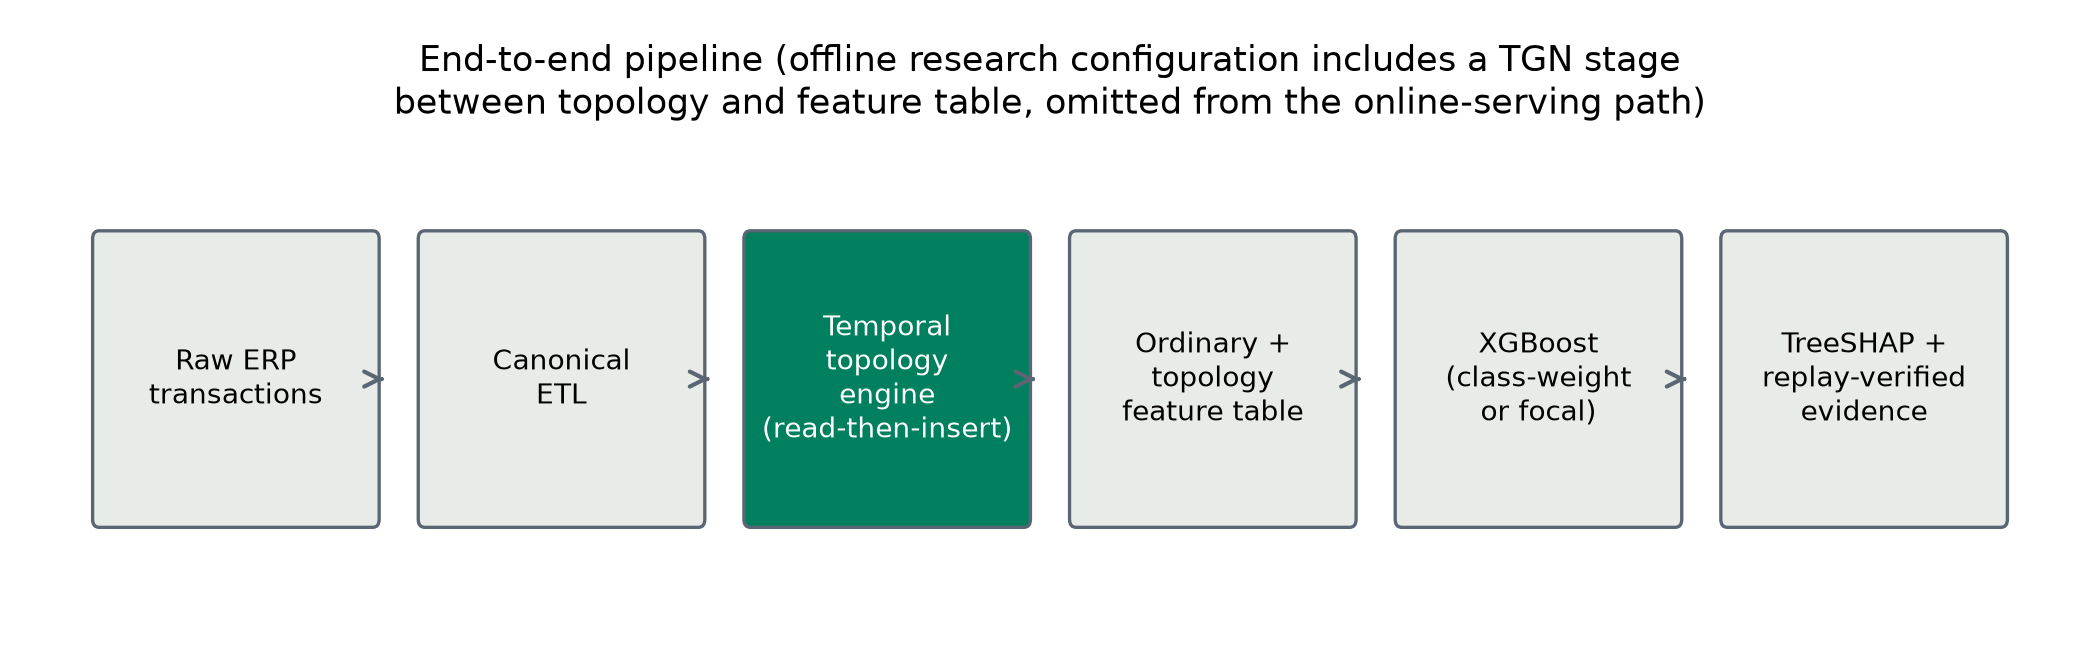
\includegraphics[width=\columnwidth]{figures/pipeline_overview.png}
\caption{End-to-end pipeline. Raw ERP transaction feeds are cleaned into a
canonical accounts/transactions schema, assembled into a temporal shadow
graph, and passed through the streaming topology engine under the
read-then-insert invariant, so that a feature is provably a function only of
transactions strictly earlier in processing order. The resulting feature
table (ordinary + topology, with offline-only TGN embeddings added for the
research configuration) feeds a gradient-boosted model; the console layer
attaches a TreeSHAP explanation and a re-derived evidence path to every
alert. The production/online bundle omits the TGN component, since its
learned memory tensor is not persisted for live inference.}
\label{fig:pipeline}
\end{figure}
%% FIGURE TODO: Six-stage left-to-right pipeline diagram: (1) Raw ERP transaction CSVs -> (2) ETL to canonical accounts+transactions schema -> (3) Temporal shadow graph (Neo4j, visualization/demo path only, never load-bearing for scoring) -> (4) Streaming topology engine, with a callout box reading "for transaction i: read features from G_{i-1}, THEN insert transaction i into G_i" -> (5) Feature table (ordinary + topology [+ TGN embeddings, offline research path only]) -> (6a) Offline XGBoost champion (topology+TGN, research/ablation use only, not servable) and (6b) Online XGBoost bundle (ordinary+topology only, actually deployed) -> forensic console alert card showing SHAP attribution bars tagged by feature family (ordinary/topology/topology-amount-derived/tgn) plus a reconstructed evidence path (cycle or fan-in) redrawn from the graph at scoring time.

\subsection{Contributions}

This paper makes five contributions, listed in the order the paper
substantiates them:

\begin{enumerate}
\item \textbf{A leakage-free streaming topology engine with a formal
read-then-insert invariant.} Every one of the engine's structural detectors
(in-/out-degree fan-in and fan-out, cycle membership and amount-conserving
cycle features, and recurring near-equal-amount ``lapping'' features) is
computed under the invariant above and guarded by an automated,
order-scrambling regression test, rather than validated only by an
after-the-fact audit.

\item \textbf{A rigorous within-dataset ablation across four heterogeneous
datasets.} The same feature engine, model family, and evaluation protocol are
applied, unchanged, to two independent real-world payment datasets, one real
ERP general-ledger dataset, and one internally generated synthetic dataset
chosen to span a deliberate spectrum of graph structure, from near-tree
(customer-to-merchant only, cycles structurally impossible) to rich,
cyclical, multi-account flows. Reporting the same probe on datasets that
differ this much in how much structure they even contain is itself part of
the evidence: a topology signal that appears only where structure is rich and
vanishes where it is sparse is more credible than one reported on a single
dataset.

\item \textbf{A calibrated synthetic ERP economy generator with an
adversarial realism audit.} To study topology-rich fraud behavior and to
probe whether synthetic data can safely augment real training sets, we build
a seeded, agent-based synthetic ERP economy whose fraud is generated from
criminal goals and evasion behavior rather than from the shapes our own
detectors look for -- avoiding the circularity of grading a detector against
data manufactured to fit it -- and subject it to an independent adversarial
review and a realism battery before using it for anything beyond sanity
checks.

\item \textbf{A production system that serves the leakage-free feature
computation online.} The same streaming engine that produces the research
feature table also backs a running ERP application and forensic audit
console, computing ordinary and topology features on live postings under the
identical read-then-insert invariant. We are explicit throughout this paper
about a consequential asymmetry: the strongest \emph{offline} research
configuration additionally includes learned temporal-graph-network (TGN)
embeddings, but the TGN's per-account memory state is not persisted, is not
guaranteed bit-reproducible across machines even under a fixed random seed
(quantified later in this paper), and is therefore
never part of what is actually served online. Every PR-AUC figure in this
paper is labeled as belonging to one of two distinct models -- the
\emph{offline champion} (topology and, where used, TGN) or the
\emph{deployed online bundle} (ordinary and topology only) -- and the two are
never conflated.

\item \textbf{Full transparency, including negative and null results.}
Alongside the positive result, we report, without softening: a dataset on
which the full model's topology addition measurably reduces PR-AUC; a
dataset whose tabular baseline is already so strong that the marginal
comparison is close to uninformative; an ablation study that is single-seed
and therefore silent on whether a small positive lift is signal or noise; a
headline structural-motif family (cycle detection) that contributes
negligible gain importance on most of the datasets studied despite being the
project's original motivating idea; and a synthetic-data augmentation
experiment whose main finding is that naive augmentation \emph{degrades}
real-data performance, with only a narrower, different transfer claim holding
up.
\end{enumerate}

\subsection{Preview of Findings}

Across the two real payment-network datasets and the real ERP ledger dataset
evaluated in the final, multi-seed model comparison, the picture is genuinely
mixed, not uniformly positive. On the sparse, customer-to-merchant payment
dataset -- structurally incapable of containing true multi-hop cycles --
adding hand-crafted topology features raises test PR-AUC from a
$0.7870 \pm 0.0700$ ordinary-feature baseline to $0.9319 \pm 0.0017$, and the
fully tuned champion configuration reaches $0.9364 \pm 0.0015$ with perfect
precision at the top 100 alerts. On the anti-money-laundering simulation
dataset, whose ordinary-feature baseline already reaches
$0.9920 \pm 0.0026$ PR-AUC, adding topology reaches a ceiling of
$1.0000 \pm 0.0000$ -- a result we flag, not celebrate, as an artifact of an
already-saturated baseline rather than evidence of a large structural effect;
the informative signal on this dataset lives in an amount-blind probe
reported later, not in this marginal comparison. On the real,
university-published SAP general-ledger dataset, the honest result runs the other way:
the ordinary-feature baseline reaches $0.1581 \pm 0.0129$ PR-AUC, and adding
topology \emph{lowers} it to $0.0717 \pm 0.0095$; only after a full
hyperparameter search and a change of imbalance mechanism does the final
champion claw back to $0.1557 \pm 0.0717$, statistically indistinguishable
from the ordinary baseline it started from. This dataset carries only 25
labeled test frauds, and we treat the result as underpowered rather than
disproving the hypothesis outright -- but we do not discard it, and we do not
let the two datasets where topology clearly helps stand in for a result that,
on this one, it measurably did not. We return to all three results with full
detail, confidence caveats, and feature-level attribution later in this
paper.

\subsection{Paper Organization}

Section~\ref{sec:related} situates this paper in the graph-based fraud
detection, class-imbalance, temporal graph network, continuous-auditing, and
explainability literatures, and argues that this paper's central gap-filling
contribution is methodological -- an explicit leakage taxonomy and a
same-architecture, multi-dataset ablation -- rather than a new graph
architecture. Later sections (not assigned to this document) develop the
leakage taxonomy and its automated guard in full, describe the four
evaluation datasets and the synthetic generator's realism audit, detail the
streaming architecture and the production ERP and forensic console, report
the ablation and augmentation experiments with complete confidence
accounting, and close with the explainability layer, limitations, and future
work.

\section{Related Work}\label{sec:related}

This section reviews five bodies of work this paper draws on -- graph-based
fraud and money-laundering detection, class-imbalance learning, temporal
graph networks, continuous auditing and ERP-centric fraud research, and
post-hoc explainability -- and closes by positioning this paper's
contribution against the first of these in particular.

\subsection{Graph-Based Fraud and Anti-Money-Laundering Detection}

The premise that fraud and laundering are relational, not point, phenomena
has produced a substantial and fast-growing graph neural network (GNN)
literature, surveyed broadly by Yuan et al.~\cite{yuan2025survey} for
GNN-based anomaly detection and specifically for financial fraud by Motie and
Raahemi~\cite{motie2024gnn}, whose systematic review taxonomizes
architectures, node/edge representations, and evaluation practices across
the field. Within that space, several recent directions are represented in
the citations this paper draws on. Devi et al.~\cite{devi2025rlgnn} fuse
reinforcement learning with a GNN backbone for real-time fraud detection,
aiming at the same online-scoring setting this paper's production console
targets. Tong et al.~\cite{tong2023financial} and Zhi et
al.~\cite{zhi2025imbalanced} both target the fraud literature's dominant
practical obstacle -- extreme class imbalance -- from the graph side,
combining GNN representations with imbalance-aware learning and,
respectively, an embedding-aware conditional GAN for synthetic minority
generation. Boyapati et al.~\cite{boyapati2025balancer} propose an
architecture-level balancing mechanism (BalancerGNN) rather than a
data-level one. Shi et al.~\cite{shi2026uncertainty} combine spatio-temporal
contrastive representation learning with explicit uncertainty
quantification, addressing a concern this paper shares -- that a bare
point-estimate fraud score is of limited use to an auditor who must decide
how much to trust it. A smaller quantum-computing strand is also
represented: Innan et al.~\cite{innan2024quantum} and Grossi et
al.~\cite{grossi2022mixed} both explore quantum and hybrid quantum-classical
graph learning for fraud classification and feature selection; both are, by
the nature of current quantum hardware, proof-of-concept studies rather than
deployment-scale systems, and we include them here for completeness of the
graph-fraud landscape rather than as a direct comparison point for the
tabular-scale production system this paper describes. Table~\ref{tab:related_gnn}
summarizes the method family and stated focus of each.

\begin{table}[t]
\centering
\small
\caption{Representative recent graph-based approaches to financial fraud and
anti-money-laundering detection cited in this paper.}
\label{tab:related_gnn}
\begin{tabular}{@{}p{0.13\columnwidth}p{0.36\columnwidth}p{0.40\columnwidth}@{}}
\toprule
\textbf{Source} & \textbf{Method family} & \textbf{Stated focus} \\
\midrule
\cite{motie2024gnn} & Systematic review & GNN architectures for financial fraud, taxonomized \\
\cite{yuan2025survey} & Survey & GNN-based anomaly detection broadly, fraud as one application \\
\cite{innan2024quantum} & Quantum GNN & Fraud classification via quantum graph circuits \\
\cite{grossi2022mixed} & Quantum-classical hybrid & Fraud detection with quantum-assisted feature selection \\
\cite{devi2025rlgnn} & RL + GNN fusion & Real-time fraud scoring via RL-guided graph policies \\
\cite{tong2023financial} & GNN + imbalance learning & Transaction-level fraud detection under class skew \\
\cite{zhi2025imbalanced} & Conditional GAN + embeddings & Synthetic minority generation for imbalanced fraud data \\
\cite{boyapati2025balancer} & Balanced GNN architecture & Architecture-level remedy for imbalanced graph classification \\
\cite{shi2026uncertainty} & Contrastive + uncertainty-aware GNN & Spatio-temporal fraud detection with calibrated confidence \\
\cite{wang2023reinforced} & RL causal explainer & Post-hoc causal explanation for GNN predictions \\
\bottomrule
\end{tabular}
\end{table}

What this literature only inconsistently reports, and rarely reports jointly,
is (i) an explicit statement of how a temporal or relational feature's
computation is bounded relative to the timestamp of the transaction it
describes, and (ii) a same-architecture ablation isolating the graph
component's marginal contribution over a tabular baseline of matched
capacity. This paper's own pre-rebuild history is direct evidence that this
omission is not merely academic: without both a formal temporal-computation
invariant and a first-class ablation, a reported gain from adding graph
structure is not distinguishable, from the outside, from a gain produced by
leakage or by an unmatched baseline. We return to this gap in
Section~\ref{sec:related-gap}.

\subsection{Class-Imbalance Learning}

Fraud labels are rare by construction -- across the four datasets used later
in this paper, positive rates range from roughly one in a thousand
transactions to just over one in a hundred -- and imbalance-handling choices
materially affect both accuracy and, importantly, its variance across
training runs. Lin et al.~\cite{lin2017focal} introduce focal loss for dense object
detection, reshaping the standard cross-entropy objective to down-weight
easy, confidently-correct examples so that training gradient is concentrated
on the hard cases; the same reshaping transfers naturally to rare-event
tabular classification and is used later in this paper's own model-selection
protocol, compared head-to-head against simple class weighting under a rule
that the two imbalance mechanisms are never combined within a single
experiment. Zhi et al.~\cite{zhi2025imbalanced}, discussed above, instead address
imbalance at the data level via conditional generative augmentation of the
minority class within a graph-aware embedding space -- a resampling family we
deliberately avoid for structural (as opposed to purely tabular) features,
since interpolating between two graph-derived feature vectors can produce a
combination -- for instance, half of a cycle -- with no physical
transaction-graph realization.

\subsection{Temporal Graph Networks}

Rossi et al.~\cite{rossi2020temporal} introduce Temporal Graph Networks (TGNs): a
memory-augmented architecture that maintains a compact, continuously-updated
state vector per node, updated via a recurrent cell as each new edge (here, a
transaction) is observed, and trained with a self-supervised link-prediction
objective rather than direct supervision on any downstream label. This paper
adopts a TGN, trained self-supervised and hence label-free, as the learned
counterpart to the hand-crafted topology detectors in its offline research
configuration: an account's TGN embedding is read \emph{before} the
transaction that updates it is folded into memory, preserving the same
temporal-ordering discipline used for the hand-crafted features, and the
embedding is deliberately restricted from access to transaction amounts so
that its contribution can be isolated from the model's known amount-driven
signal. Later sections of this paper are explicit, however, that this
paper does not treat the TGN as free to deploy: floating-point
non-determinism in CPU-trained recurrent updates compounds over an
epoch's worth of transactions to the point that TGN-derived embeddings
retrained on the same, fixed random seed but on a different machine are not
bit-reproducible against a previously committed model, and the memory state
itself is not persisted for streaming inference -- both properties that keep
the TGN a research-arm-only component in this paper's accounting, never part
of the production-served model.

\subsection{Continuous Auditing and ERP-Centric Fraud Research}

A parallel, older literature addresses fraud and control failures from the
audit and information-systems side rather than the machine-learning side.
Vasarhelyi et al.~\cite{vasarhelyi2012acceptance} study the acceptance and adoption of
continuous auditing techniques by internal auditors, documenting that
technique sophistication alone does not guarantee organizational uptake --
relevant context for this paper's emphasis on an audit console that surfaces
not just a score but a reconstructed, human-checkable evidence path for every
alert, since an unexplained score is exactly the kind of output that
technique-adoption research finds auditors distrust. Jawad et al.~\cite{jawad2024erp}
review machine-learning-driven optimization of ERP systems broadly, situating
fraud scoring as one of several ML use cases layered on ERP data (alongside
demand forecasting, process mining, and anomaly detection in master data) and
noting that most such deployments remain post-hoc analytics layered outside
the transactional system of record rather than integrated into it --
precisely the gap this paper's production console, built to score
transactions at posting time rather than in a downstream batch job, is meant
to close. Mamakou et al.~\cite{mamakou2024postimplementation} evaluate ERP systems
post-implementation from internal auditors' own perspective, underscoring
that an ERP-adjacent tool's practical value is judged by auditors against
criteria -- traceability, explainability of automated outputs, and
compatibility with existing control frameworks -- that a raw model accuracy
number does not, by itself, satisfy. Together, this literature motivates why
this paper treats the explanation and evidence-reconstruction layer as a
first-class deliverable rather than an add-on to a scoring model.

\subsection{Explainability for Tree and Graph Models}

An accuracy figure, however well validated, does not on its own justify
opening a fraud investigation; the audience for a fraud alert needs to know
\emph{why} a transaction scored highly. Lundberg and Lee~\cite{lundberg2017unified} unify a
family of additive feature-attribution methods under the Shapley-value-based
SHAP framework, providing a game-theoretic, locally accurate decomposition of
a model's output into per-feature contributions. Lundberg et al.~\cite{lundberg2020local}
extend this to TreeSHAP, an algorithm that computes exact (not sampled or
approximated) Shapley values for tree-ensemble models in low-order polynomial
time -- a property this paper relies on directly, since it is a
determining factor, alongside raw predictive accuracy, in this paper's choice
of a gradient-boosted tree ensemble as the final classifier head over an
end-to-end neural alternative: exact, cheap attribution is available for
trees in a way it is not for most deep architectures. On the graph side,
Wang et al.~\cite{wang2023reinforced} propose a reinforcement-learning-based causal
explainer for GNN predictions, targeting a complementary explainability
problem -- explaining which subgraph structure drove a graph model's own
decision, rather than which tabular feature drove a downstream classifier's
decision. This paper's design deliberately sidesteps needing a GNN-native
explainer of that kind for its production scoring path, feeding learned graph
signal into TreeSHAP-explainable tree features rather than explaining a graph
model's decision directly; the graph itself is instead re-rendered for the
auditor as the literal evidence path (the reconstructed cycle or fan-in
structure a given alert is attributed to), verified independently at display
time against the same stored feature state the score was computed from.

\subsection{Positioning of This Work}\label{sec:related-gap}

Read across the sections above, the recurring shape of the gap this paper
targets is consistent. Model novelty in the graph-based fraud literature is
abundant: new architectures, new imbalance-handling mechanisms, new
uncertainty-quantification and explainability layers all appear at a healthy
pace, and the citations above are one small, recent sample of that pace. What
is comparatively scarce, and what this paper is built around supplying, is
methodological accounting for two specific threats to validity that are easy
to state and easy to violate silently: whether a temporal or relational
feature could, even in principle, have depended on information from after
the event it describes, and whether an architecture's graph component is
being compared against a tabular baseline of genuinely matched capacity
rather than a weaker straw-man. Neither threat is exotic -- this paper's own
preliminary iteration fell to both simultaneously, with a future-looking
feature ranked among its most important, before an internal audit caught it
-- and neither is fully addressed by adding a leakage \emph{test} after
model development, since a test can only catch a violation the engineer
thought to check for. The response this paper takes is architectural rather
than remedial: a read-then-insert invariant enforced in the feature engine
itself (Section~\ref{sec:intro}), guarded by an automated regression test
rather than a one-time audit, and a within-dataset, same-architecture
ablation run identically across four structurally different datasets rather
than a single headline comparison. This paper's technical components --
hand-crafted topology detectors, a TGN~\cite{rossi2020temporal},
gradient-boosted trees, focal-loss and class-weight imbalance handling
\cite{lin2017focal}, and TreeSHAP attribution \cite{lundberg2020local} --
are consequently adaptations of established techniques rather than new
architectures in their own right. The contribution is the discipline wrapped
around them, and the willingness, evidenced throughout this paper, to report
what that discipline finds even when it is a negative result on the very
dataset the project's original hypothesis was built to explain.

\section{Proposed Model and Methodology}\label{sec:methodology}

\subsection{Problem Formulation and Leakage Taxonomy}\label{sec:problem}

\subsubsection{Task Definition}

We formalize fraud detection on ERP and payment data as per-transaction
binary classification over a temporal, directed, attributed multigraph. Let
$\mathcal{V}$ denote the set of entities (accounts, vendors, G/L codes, or
customers, depending on the dataset) and let
$\mathcal{D} = \{e_1, e_2, \dots, e_N\}$ denote the transaction set, where
each transaction is a tuple
\[
e_i = (u_i, v_i, t_i, a_i, \mathbf{c}_i, y_i),
\]
with origin $u_i \in \mathcal{V}$, destination $v_i \in \mathcal{V}$,
timestamp $t_i \in \mathbb{R}$ (or an ordinal step/day index --
Section~\ref{sec:datasets} details each dataset's time axis), amount
$a_i \in \mathbb{R}_{>0}$, an auxiliary attribute vector $\mathbf{c}_i$
(transaction/document type, channel), and a binary label
$y_i \in \{0,1\}$ recording confirmed fraud. Transactions induce a directed
multigraph $G = (\mathcal{V}, \mathcal{D})$ that grows monotonically in
time; we write
\[
G_{\le T} \;=\; \bigl(\mathcal{V},\, \{\, e_j \in \mathcal{D} : t_j \le T \,\}\bigr)
\]
for the graph state immediately after every transaction up to and
including time $T$ has posted. The task is to fit a scoring function
$f_\theta : \mathbb{R}^d \to [0,1]$, applied to a feature vector
$x_i = \phi(e_i, G)$ extracted for each transaction, that approximates
$\Pr(y_i = 1 \mid x_i)$. Three feature families compose $x_i$ in this
project: ordinary transaction attributes ($a_i$, $\mathbf{c}_i$, calendar
features), structural/topology statistics computed from the graph (degree,
fan-in/out, lapping recurrence, cycle membership), and, where used, learned
temporal-graph embeddings (TGN) \cite{rossi2020temporal}. The graph
neural network literature has repeatedly reported structure-aware models
outperforming tabular baselines on financial fraud tasks
\cite{motie2024gnn,yuan2025survey}, almost always without an explicit audit
of the temporal-leakage failure modes formalized below; the dataset roster
in Section~\ref{sec:datasets} is chosen so that a fair, leakage-controlled
version of that comparison is possible across a genuine range of
structural richness. With the class prior $\Pr(y=1)$ ranging from roughly
0.12\% to 1.21\% across the real datasets studied here
(Table~\ref{tab:datasets}), we follow standard practice for severely
imbalanced classification \cite{bishop2006pattern} and evaluate with
threshold-independent ranking metrics (PR-AUC / average precision,
precision@$k$) rather than accuracy or a fixed decision threshold; the full
metric discussion and the modeling protocol built on it are given later in
this paper.

\subsubsection{Leakage-Free Feature Computation}

The single methodological requirement that dominates every other design
decision in this project is that $\phi$ must not use information
unavailable at the instant $e_i$ posts. We state this precisely.

\begin{quote}
\textbf{Definition (leakage-free feature map).} A feature map $\phi$ is
\emph{leakage-free} with respect to $\mathcal{D}$ if, for every transaction
$e_i \in \mathcal{D}$,
\[
\phi(e_i, G) \;=\; \phi(e_i, G_{\le t_i})
\]
for any $G \supseteq G_{\le t_i}$ -- that is, $\phi$'s output for $e_i$ is
invariant to which transactions with $t_j > t_i$ are or are not present in
the graph.
\end{quote}

Operationally we enforce this with a single streaming pass over
$\mathcal{D}$ in non-decreasing timestamp order: for each $e_i$, (1)
\emph{read} $x_i = \phi(e_i, G_{<t_i})$ against the graph state already
committed, then (2) \emph{insert} $e_i$'s edge and any derived state
(running counts, expanding means, open cycle candidates) before moving to
$e_{i+1}$. This read-then-insert ordering makes look-ahead structurally
impossible rather than merely policy-forbidden -- no code path exists
through which a later transaction's data can reach an earlier
transaction's feature vector. Two corollaries follow directly and are
enforced throughout the engine: (a) no statistic used in a feature
computation -- mean, standard deviation, per-account baseline, Benford
digit distribution -- may be computed once over the whole dataset; every
such statistic must be expanding or rolling over the past only, and (b)
when a structure (a cycle, a lapping sequence) is only detectable once its
final edge posts, its signal attaches to that \emph{completing}
transaction, never retroactively to the earlier transactions that merely
participated in it. Train/validation/test partitioning follows the same
discipline: splits are chronological -- train on the earliest period,
validate on the next, test on the latest -- never a randomly shuffled
$k$-fold, a protocol documented elsewhere to silently leak the future into
the past on time-evolving, dynamic fraud data \cite{jesus2022turning}.

\subsubsection{Leakage Taxonomy: Two Failure Modes in the Predecessor System}

An earlier iteration of this codebase reported headline metrics as strong
as $\mathrm{ROC\text{-}AUC} \approx 0.997$ on its flagship dataset and
concluded that graph topology was fraud detection's ``ultimate
differentiator.'' A pre-registration audit of that system's own artifacts
found the opposite: its topology detectors scored essentially 0.0 feature
importance, and every reported number was contaminated by two independent,
stacked leakage mechanisms. We name them Leak Class A and Leak Class B and
treat their elimination as this project's primary internal-validity
requirement.

\textbf{Leak Class A -- whole-graph feature computation.} The predecessor's
topology detectors ran once over the \emph{entire} graph, with no
$t_j \le t_i$ restriction anywhere, and each detected structure's signal
was written back to every member transaction, including its earliest ones
-- a cycle only observable once closed was nonetheless flagged on the edge
that opened it, directly violating the definition above. Two concrete
symptoms make the violation unambiguous: (i) a feature literally named
\texttt{time\_to\_next} -- the number of seconds until each account's
\emph{next} transaction -- ranked among the top five features by
importance; no detector can know the gap to a future transaction without
having already observed it. (ii) Every z-score / anomaly feature was
standardized against a whole-dataset mean and variance computed once, so a
transaction dated on day one was scored against a ``normal'' baseline that
included transactions from every later day, test period included.

\textbf{Leak Class B -- modeling-protocol leakage.} Four compounding,
confirmed malpractices were present in all five of the predecessor's
training scripts. (i) SMOTE oversampling and class-weighting were applied
\emph{simultaneously}, double-correcting for imbalance; because SMOTE's
$k$-nearest-neighbor interpolation was applied indiscriminately to
topology columns, it manufactured physically impossible points (a
synthetic transaction with, e.g., 0.4 of a closed cycle) that eased the
learned boundary without corresponding to any real fraud pattern. (ii)
Every reported metric used the library's default 0.5 decision threshold
(\texttt{.predict()}), never a threshold selected on held-out data --
meaningless when the positive class is 0.1--1.2\% of rows, since 0.5 is
not an operating point anyone chose. (iii) Cross-validation used
\texttt{StratifiedKFold} with shuffling and the timestamp column dropped
before fitting, so folds routinely trained on transactions dated after the
ones being scored, layering random-future leakage directly on top of Leak
A. (iv) Models were selected by F1 at that same fixed 0.5 threshold rather
than a threshold-independent, imbalance-appropriate ranking metric, which
rewards whichever leak-inflated configuration happens to look best at an
arbitrary cutoff rather than the one that generalizes.

\textbf{Why each invalidates the reported numbers.} Leak A inflates
apparent predictive power because the model is not learning what is
knowable at the moment an investigator would act -- it is learning the
correlation between a label and events that, by construction, occur after
the label's determining moment; the resulting metric is not an estimate of
deployable detection ability at all. Leak B compounds this at the
evaluation layer: synthetic minority points generated from a distribution
informed by the whole, undifferentiated dataset bias the decision boundary
toward the very examples later used to measure it; shuffled folds directly
violate the temporal ordering a fraud investigation depends on; and
selecting the ``best'' configuration by a metric computed under both prior
leaks means every design choice in the pipeline was made with implicit
knowledge of the answer it would later be graded on. Under datasets this
imbalanced -- as few as 19--25 confirmed fraud transactions in a single
evaluation split for SAP W\"urzburg (Section~\ref{sec:datasets}) -- even a
handful of leaked examples can move a headline metric by tens of points,
which is precisely the failure mode the leakage-free construction above,
and the ablation protocol built on it, are designed to make structurally
impossible rather than merely audited for after the fact.

%% FIGURE TODO: two-track timeline diagram. Top track: the correct
%% read-then-insert order -- for a transaction at time T, an arrow reads
%% features from graph state at T (pointing only left/backward in time),
%% then a second arrow commits/inserts the edge, moving strictly
%% left-to-right with no arrow ever pointing forward. Bottom track: the
%% predecessor system's Leak A pattern -- a completed-cycle icon at day 40
%% sends an arrow backward past day 40 to overwrite/attach to feature
%% values at day 3, visually contrasting causal vs. acausal attribution of
%% the same structure.
\begin{figure}[t]
  \centering
  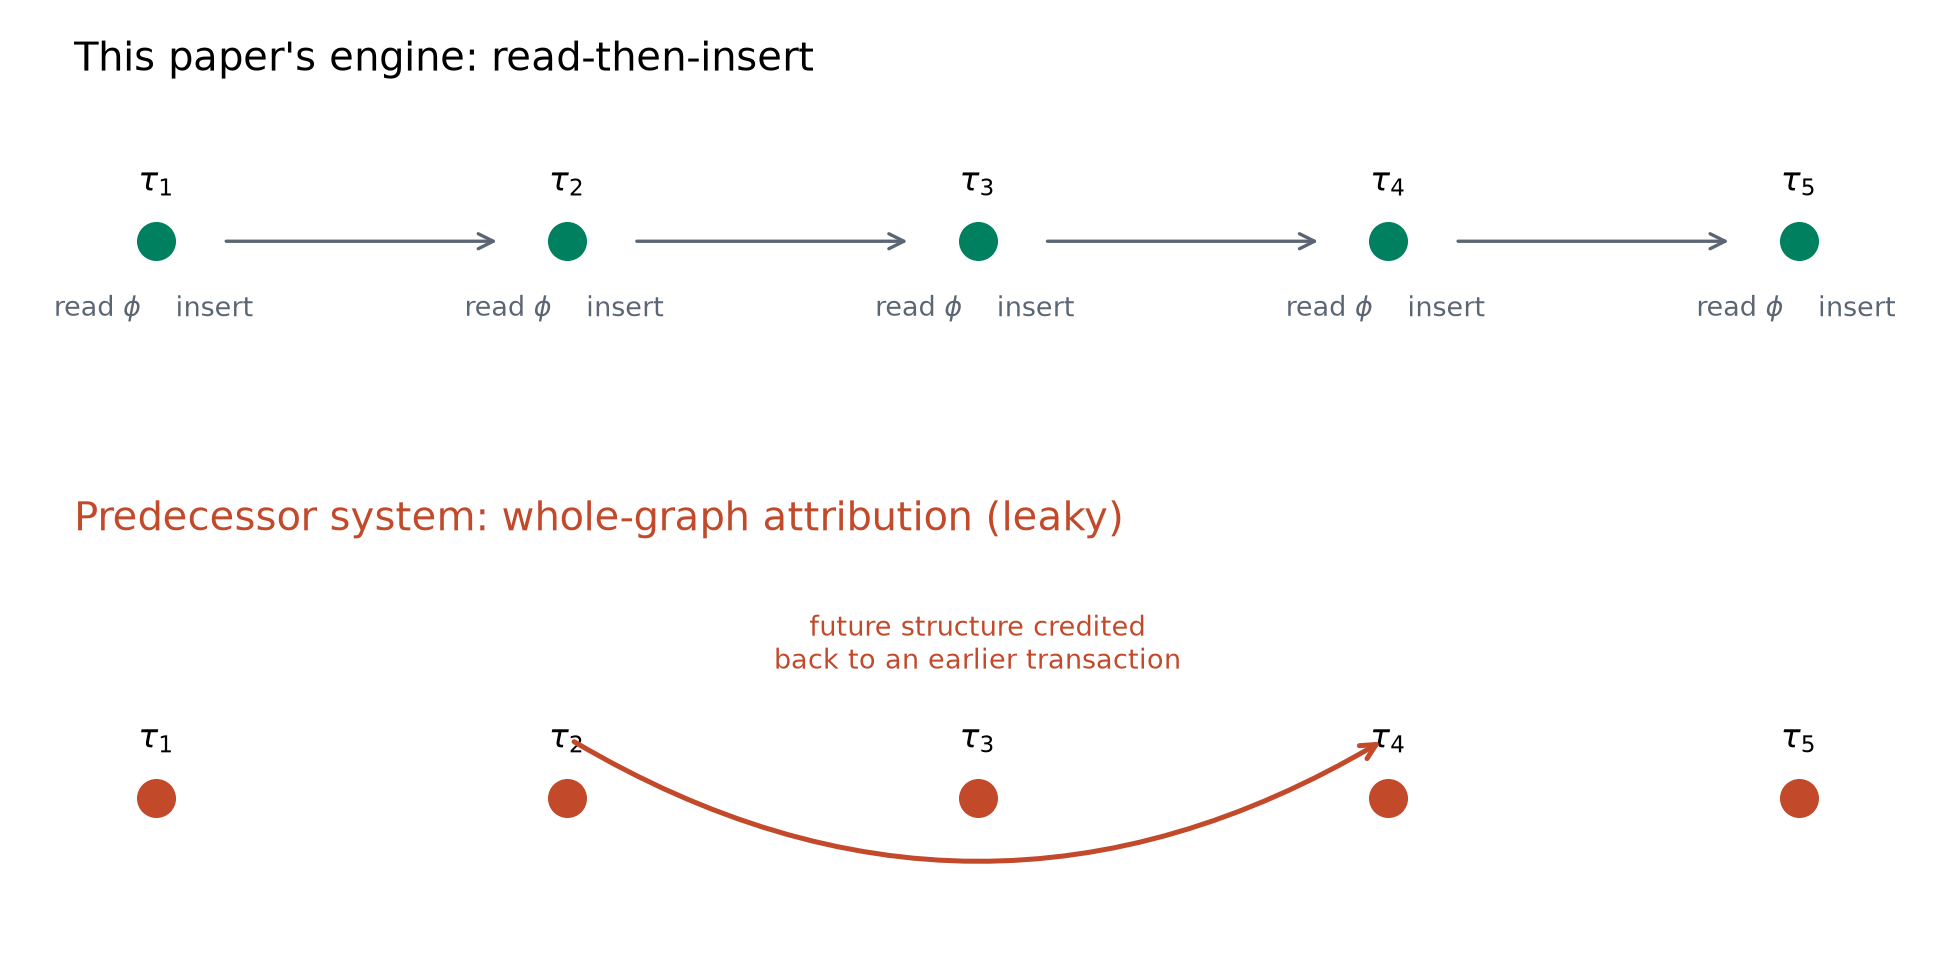
\includegraphics[width=\columnwidth]{figures/leakage_timeline.png}
  \caption{Read-then-insert feature computation (top) versus the
  predecessor system's whole-graph attribution (bottom), which credited a
  structure's signal back to transactions that occurred before the
  structure existed.}
  \label{fig:leakage_timeline}
\end{figure}

\subsection{Datasets}\label{sec:datasets}

\subsubsection{Overview and the Topology-Richness Spectrum}

Because the hypothesis under test is whether \emph{graph structure} carries
predictive signal beyond a strong tabular baseline, the dataset roster is
presented here as points along a topology-richness spectrum rather than as
an arbitrary convenience sample: from IBM AML, whose sender and receiver
identifiers occupy a near-unified account namespace supporting true
multi-hop cycles, down to PaySim, whose transaction graph is a near-forest
of one-off pairs. Table~\ref{tab:datasets} summarizes the four datasets
computationally profiled end-to-end in this study -- IBM AML, BankSim, SAP
W\"urzburg, and PaySim -- drawn from a single calibration pass over each
dataset's fully processed transaction table
(\texttt{calibration\_reference.json})
\cite{altman2023realistic,lopezrojas2014banksim,lopezrojas2016paysim}.
\emph{Kind} records each dataset's native graph topology: \texttt{Transfer}
(a directed account$\to$account graph, as in a payments network),
\texttt{Bipartite} (two structurally disjoint node classes with no
possibility of reciprocation or cycles), or \texttt{ERP ledger} (the
document-to-ledger-account bipartite structure specific to double-entry
ERP postings). \emph{NS Overlap} is the fraction of an account
namespace's senders that also appear as receivers -- the diagnostic this
project uses to certify whether same-entity cycles are even structurally
detectable; the predecessor system failed exactly this check by splitting
senders and receivers into disjoint node types, making a loop
$A\to B\to A$ structurally invisible regardless of how good its topology
engine was. \emph{Reciprocity} is the fraction of unique
(sender, receiver) pairs for which the reverse pair also transacted. Of
the four datasets in Table~\ref{tab:datasets}, only PaySim was profiled
without being modeled (Section~\ref{sec:paysim}).

\begin{table}[t]
\centering
\small
\caption{Graph-topology and scale summary of the four real datasets
computationally profiled in this study (source:
\texttt{calibration\_reference.json}). Amounts are in each dataset's
native units and are not comparable across datasets.}
\label{tab:datasets}
\resizebox{\columnwidth}{!}{%
\begin{tabular}{lccccccccc}
\toprule
Dataset & Kind & Fraud \% & $N_{\text{fraud}}$ & $N_{\text{txn}}$ & $N_{\text{acct}}$ & Amt.\ Med. & Benford MAD & NS Overlap & Recip. \\
\midrule
IBM AML       & Transfer    & 0.130 & 1{,}719 & 1{,}323{,}234 & 9{,}999       & 156.71      & 0.0758 & 0.9927 & 0.0446 \\
BankSim       & Bipartite   & 1.211 & 7{,}200 & 594{,}643     & 4{,}162       & 26.90       & 0.0319 & 0.0000 & 0.0000 \\
SAP W\"urzburg & ERP ledger & 0.124 & 248     & 200{,}629     & 59{,}883      & 1{,}975.80  & 0.0385 & 0.0000 & 0.0000 \\
PaySim        & Transfer    & 0.129 & 8{,}213 & 6{,}362{,}620 & 9{,}073{,}900 & 74{,}871.94 & 0.0142 & 0.0002 & 0.0000 \\
\bottomrule
\end{tabular}%
}
\end{table}

\subsubsection{IBM AML}

IBM AML is generated by the AMLSim multi-agent simulator and released as a
synthetic-but-structurally-realistic anti-money-laundering benchmark
\cite{altman2023realistic}. Its 1{,}323{,}234 transactions connect 9{,}999
accounts with a sender/receiver namespace overlap of 99.27\% -- the same
account IDs act as both senders and receivers almost everywhere, the
pre-condition this project treats as necessary for account-to-account
cycle detection to be structurally possible at all. Every transaction
carries the type \texttt{TRANSFER}; time is an integer day index over a
199-day span. At a fraud rate of 0.130\% (1{,}719 of 1{,}323{,}234), IBM
AML is this project's richest-structure testbed and the dataset on which
the topology hypothesis is given its best chance to succeed. It also
exhibits the sharpest amount anomaly of any dataset studied: fraud amounts
have median 10.60 and mean 9.76, against a full-population median of
156.71 and a mean of 115{,}988.18 (99th percentile 1{,}854{,}724.69) --
fraud in IBM AML clusters in a narrow, near-zero-value band while the
legitimate population is heavily right-skewed toward large transfers. We
read this as an artifact of the AMLSim generator's labeling convention
rather than a general property of laundering behavior, and it materially
shapes the ablation results discussed later in this paper: an
amount-based baseline that expects fraud to look large is directionally
wrong on this dataset, which is exactly what motivates evaluating an
amount-blind probe to isolate topology's contribution independent of this
artifact.

\subsubsection{BankSim}

BankSim is an agent-based simulation of a bank payment network built
specifically for fraud-detection research \cite{lopezrojas2014banksim}.
Its 594{,}643 transactions connect customer accounts (prefix \texttt{C})
to merchant accounts (prefix \texttt{M}) -- two structurally disjoint node
classes, so namespace overlap and pair reciprocity are both exactly 0.0
and no customer-to-customer or merchant-to-merchant cycle can exist by
construction. BankSim therefore serves this study as the sparse control:
any predictive lift topology features provide here must come from
bipartite-graph statistics (degree, fan-in/out, recurring near-equal
``lapping'' amounts) rather than from cycles, since cycles are
structurally unavailable. Its fraud rate, 1.211\% (7{,}200 of 594{,}643),
is the highest of the four real datasets, and its amounts are the smallest
in scale (median 26.90).

\subsubsection{SAP W\"urzburg}

SAP W\"urzburg is a real, publicly released SAP ERP transaction ledger and
is the only dataset in this study drawn from an actual production
accounting system rather than a simulator -- the setting continuous-
auditing research argues automated, always-on control monitoring should
target \cite{vasarhelyi2012acceptance}, and one that broader ERP-analytics
surveys still treat as an emerging rather than mature application of
machine learning \cite{jawad2024erp,mamakou2024postimplementation}. Its
graph is a document-to-account bipartite structure native to double-entry
bookkeeping: each posting document fans out to a small number of line
items (out-degree median 2.0, 99th percentile 10.0) that land on accounts,
a minority of which absorb a disproportionate share of postings (in-degree
99th percentile 43{,}706.7, maximum 46{,}554, against 59{,}883 distinct
account identifiers in total) -- a small core of heavily used ledger
accounts against a long tail of low-traffic counterparty accounts. With
only 248 confirmed frauds among 200{,}629 postings (0.124\%), SAP
W\"urzburg is this project's thinnest fraud signal by count, and, as the
ablation study reported later in this paper shows in full, the one real
dataset on which the full-model topology lift is measured
\emph{negative}. Two different SAP W\"urzburg train/validation/test
partitions appear elsewhere in this paper and should not be confused: the
chronological, partition-aware split used in the within-dataset ablation
study yields 120{,}411/40{,}137/40{,}139 rows
(\texttt{ablation.json}), while the multi-seed split used for final
champion-model selection yields 120{,}341/40{,}114/40{,}116 rows on the
same source file under a different, non-partition-aware split procedure
(\texttt{final\_champions.json}); both carry the same fraud counts by
split (204/19/25). We flag the discrepancy here so it does not appear
silently across two disconnected tables.

\subsubsection{IBM AML: Kaggle Reproduction Variant}

A second, independently downloaded instance of the IBM AML benchmark --
sourced directly from its Kaggle mirror rather than from the AMLSim-format
repository export behind the headline IBM AML numbers above -- was
processed during this build as a reproduction check on the deployed
\emph{online} scoring bundle, never as a source of headline results. The
two sources use different raw schemas (\texttt{TX\_ID}/
\texttt{SENDER\_ACCOUNT\_ID}-style AMLSim export versus the Kaggle
\texttt{HI-Small\_Trans.csv} layout) and are, in general, different
simulator draws; we report results under the separate label
\texttt{ibm\_aml\_kaggle} throughout, and none of its numbers are merged
into or averaged with \texttt{ibm\_aml}'s. For contrast -- though the two
are not directly comparable -- the offline champion model trained on the
primary \texttt{ibm\_aml} source, which includes TGN embeddings and, since
its TGN memory state is never persisted to disk, is not servable online at
all (a limitation discussed in full elsewhere in this paper), reaches a
saturated test PR-AUC of 1.00; that ceiling is itself uninformative given
the baseline's own 0.990 saturation (also discussed later in this paper).
\texttt{ibm\_aml\_kaggle}'s \emph{online} (ordinary+topology, non-TGN)
bundle -- the only kind of bundle this project ever serves in production
(\texttt{online\_bundles.json}) -- reaches a materially lower test PR-AUC
of 0.512 ($\pm$0.067 over three seeds, 26 features), consistent with both
the missing TGN component and the fact that the two \texttt{ibm\_aml}
variants are different simulator draws, not repeated measurements of the
same result.

\subsubsection{PaySim: Profiled, Not Modeled}\label{sec:paysim}

PaySim simulates a mobile-money transfer network at substantially larger
scale than any other dataset in this study -- 6{,}362{,}620 transactions
over 9{,}073{,}900 accounts \cite{lopezrojas2016paysim}, where almost
every transaction is the only time its particular (sender, receiver) pair
ever transacts (namespace overlap 0.0002, zero pair reciprocity, zero
repeat-pair transaction fraction). Its fraud rate, 0.129\% (8{,}213 of
6{,}362{,}620), sits in the same narrow band as IBM AML and SAP
W\"urzburg, but its graph is a near-forest at the opposite end of the
topology-richness spectrum from IBM AML: with essentially no repeated
edges between the same two accounts, most multi-hop structural detectors
(cycles, recurring lapping, degree accumulation) have little to attach to
before a transaction resolves. Consistent with this project's tiered
dataset plan, PaySim was carried through the ETL and topology-profiling
stages reported in Table~\ref{tab:datasets} but was never carried into
model training or the ablation study reported later in this paper; no
PR-AUC, precision@$k$, or lift number exists for it anywhere in this work,
and its row in Table~\ref{tab:datasets} should be read purely as a
structural reference point completing the spectrum, not as a modeling
result.

\subsubsection{The Synthetic Economy: synth\_erp}

\texttt{synth\_erp} is this project's own agent-based synthetic ERP
economy, spanning 39{,}256 accounts, generated deliberately \emph{after}
the real-data ablation protocol was designed, specifically to avoid the
circularity risk of injecting fraud in the exact shape a detector is built
to find -- a trap the predecessor system fell into by labeling injected
fraud literally \texttt{"Circular Payment"} or \texttt{"Lapping"}. Fraud is
instead generated from simulated criminal intent and evasion behavior, and
an independent adversarial leakage probe run against the resulting table
reports no exploitable single- or two-feature giveaway rule
(\texttt{leak\_flag: false}, \texttt{synth\_erp\_realism.json}); the worst
rule found, \texttt{tx\_type=transfer \& dest\_created\_midyear}, reaches
only 9.29\% precision at 43.75\% recall of fraud, a $19\times$ lift over
the 0.488\% base rate that is unremarkable next to a genuinely leaking
rule. At 1{,}148{,}503 transactions and a fraud rate of 0.488\% --
deliberately elevated above any real dataset's 0.124--1.211\% range to
keep minority-class training stable -- \texttt{synth\_erp} was built with
a near-unified account namespace (0.941 overlap) and the highest pair
reciprocity of any dataset in this study (0.136), by design, to give
topology detectors rich structure to find. Its amount distribution is, if
anything, \emph{too} clean relative to real data: a Benford MAD of 0.0047
is roughly three to sixteen times lower than any real dataset's
(0.0142--0.0758, Table~\ref{tab:datasets}) -- more compliant with
Benford's law than any of the messy real ledgers it is meant to
approximate, a known limitation of amount generation in synthetic
financial data that we surface rather than smooth over. Per the project's
own circularity safeguard, \texttt{synth\_erp} is used only for
training-time augmentation and stress-testing experiments, reported later
in this paper; it is never a source of this paper's headline ablation
claim, which is evaluated exclusively on the three real, independently
sourced datasets in Table~\ref{tab:datasets} that were carried into
modeling, plus SAP W\"urzburg's ERP-native structure specifically.

%% FIGURE TODO: scatter/bubble plot, x-axis = sender/receiver namespace
%% overlap (0 to 1), y-axis = pair reciprocity (0 to ~0.14), bubble area
%% = n_transactions (log scale), one labeled bubble per dataset (ibm_aml,
%% banksim, sap_wurzburg, paysim, synth_erp) -- visualizing the
%% topology-richness spectrum the roster is chosen to span, with ibm_aml
%% and synth_erp anchoring the structure-rich corner and banksim/
%% sap_wurzburg/paysim clustered at the structurally sparse origin.
\begin{figure}[t]
  \centering
  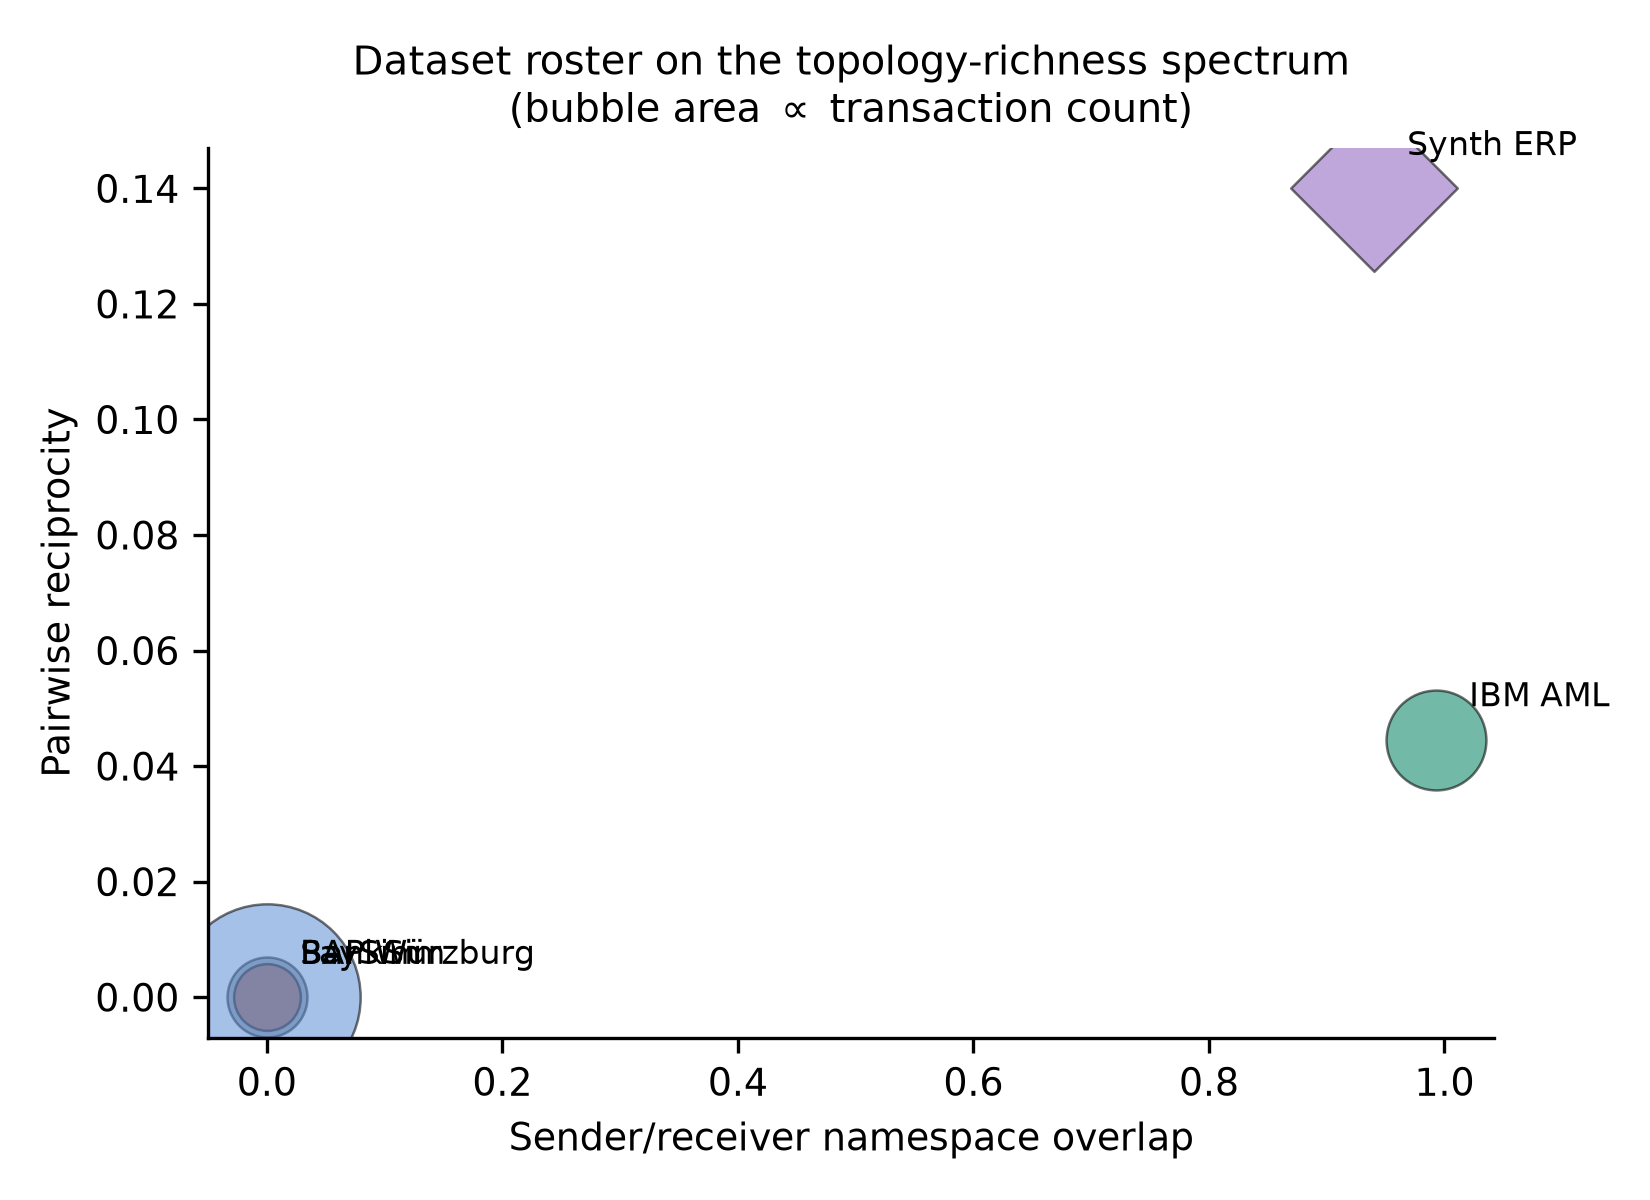
\includegraphics[width=\columnwidth]{figures/dataset_topology_spectrum.png}
  \caption{The five datasets positioned on the two structural axes this
  study uses to justify the roster: sender/receiver namespace overlap
  ($x$) and pair reciprocity ($y$), bubble area proportional to
  transaction count. IBM AML and \texttt{synth\_erp} anchor the
  structure-rich end; BankSim, SAP W\"urzburg, and PaySim anchor the
  structurally sparse end.}
  \label{fig:topology_spectrum}
\end{figure}

\subsection{Leakage-Free Temporal Topology Engine}\label{sec:engine}

A transaction does not reveal fraud in isolation; the same transfer can be
ordinary in one account context and the closing leg of a laundering cycle in
another. Graph-based fraud detection formalizes this by treating the ledger as
a network of who-paid-whom and searching for structural motifs — cycles,
fan-in collection points, rapid pass-through chains — that a row-wise view
cannot see~\cite{motie2024gnn,yuan2025survey,salih2021survey}. The difficulty
is computing such motifs \emph{as they would have been visible at the time},
without letting the completed, labeled dataset's hindsight leak into a
feature that is supposed to represent an auditor's knowledge at transaction
time. This section describes the streaming component of the Self-Auditing
Ledger that does this — the Temporal Topology Engine — and states, precisely
and with the project's own evidence, which of its thirteen output features
actually earn their keep.

The engine operates on the canonical edge list produced by ETL: one row per
transaction, with a source account, a destination account, a timestamp, an
amount, and (for training data) a fraud label. It is deliberately \emph{not}
a graph neural network and does not touch Neo4j; it is a single linear pass
over the sorted edge stream, maintained in pure Python/NumPy, that emits one
feature vector per transaction. Two data structures carry all state across
that pass: a trailing-window directed multigraph, \texttt{WindowGraph}, and a
per-account rolling amount memory, \texttt{LapMemory}. Both are described
below, followed by the thirteen features they jointly produce, the
structure/amount split used to keep the later ablation honest, and the
feature-importance result — including a null result the project does not
soften.

\subsubsection{The Leakage Invariant: Read, Then Insert}\label{sec:engine-invariant}

CLAUDE.md's rule 4 states the requirement in one sentence: a transaction's
features may depend only on transactions with \texttt{timestamp <=} its own.
The engine satisfies this not as a coding convention that a future edit could
quietly violate, but as a structural property of a single loop body. Edges
are pre-sorted by \texttt{(timestamp, transaction\_id)} — the ETL writes them
in this order with a stable sort, and the feature-assembly stage re-sorts
defensively if that invariant is ever violated upstream. The engine then
iterates \texttt{for i in range(n)} and, for transaction $i$, executes
exactly two kinds of statement in exactly one order:

\begin{enumerate}
  \item \textbf{Read.} Query \texttt{WindowGraph} for $i$'s fan-in, fan-out,
  destination in-degree, source out-degree, and (if $\mathrm{src}_i \neq
  \mathrm{dst}_i$) run the bounded cycle search; query \texttt{LapMemory} for
  the recurrence of $i$'s amount against each endpoint's rolling history.
  \item \textbf{Insert.} Only after every read above returns does the engine
  call \texttt{WindowGraph.add(t, u, v, amount)} and
  \texttt{LapMemory.record(\ldots)} for transaction $i$ itself.
\end{enumerate}

Because \texttt{add} for edge $j$ is called only during iteration $j$, and
iterations execute strictly in order $0, 1, \ldots, n-1$, the graph state
visible to iteration $i$'s reads is, by induction, exactly $\{j : j < i\}$
minus whatever \texttt{evict} has aged out — never a superset, and in
particular never anything from an iteration that has not yet run. No branch
of the loop calls \texttt{add} or \texttt{record} ahead of the paired reads
for the same $i$, and \texttt{evict} only removes edges whose timestamp falls
below \texttt{now - window}; it has no code path that admits an edge, only
ones that retire old ones. This is what we mean by \emph{leakage-free by
construction}: the claim does not rest on trusting that every caller remembers
to query before mutating, or on empirically observing no leak on the datasets
at hand — it follows from the fixed order of two statements inside one loop,
for any input that satisfies the pre-sort precondition. \texttt{LapMemory}
enforces the identical discipline: \texttt{recurrence(acct, amount)} is
always read before the same call site's \texttt{record(acct, amount,
counterparty)}. For SAP Würzburg, whose synthetic per-run time axis (encoded
as $\mathrm{run\_index}\times 10^{6} + \text{seconds-since-midnight}$) is not
a real cross-run chronology, both structures are additionally discarded and
rebuilt at every \texttt{run\_id} boundary, so a document in run 214 can never
borrow structural context assembled from a different, unrelated ledger run.

This constructive guarantee is checked, not merely asserted: an automated
leakage test (\texttt{topology.leakage\_test}) re-derives the same feature
table twice on real, built data — once truncated at the halfway point, and
once with every transaction \emph{after} the halfway point corrupted (shuffled
endpoints, amounts overwritten with an out-of-range sentinel) while
timestamps and row order are preserved — and asserts the first half's
features are byte-identical in both cases. This is deliberately redundant
with the constructive argument above: the constructive argument is the proof
that leakage is impossible for any input; the test is a regression guard that
would fail loudly if a future refactor moved a read after an insert. It has
run green throughout the build.

\subsubsection{The Trailing-Window Graph}\label{sec:engine-windowgraph}

\texttt{WindowGraph} holds a directed multigraph restricted to a trailing
time window $[\mathrm{now} - w, \mathrm{now}]$, where $w$ is a per-dataset
constant (7 days for IBM AML; 7 steps for BankSim, whose control role
requires \texttt{in\_cycle} to be identically zero everywhere since its
graph is customer$\to$merchant bipartite; 24 steps $=1$ day for PaySim; and
unbounded \emph{within} a run for SAP Würzburg, whose runs are short enough
that no window truncation is needed). Internally it keeps adjacency as
per-node dictionaries of neighbor multiplicities, so fan-in/fan-out (count of
\emph{distinct} counterparties) and weighted in-/out-degree (count
\emph{with} multiplicity) are both $O(1)$ lookups against the current
window state, and a deque of \texttt{(timestamp, u, v)} triples in arrival
order lets \texttt{evict(now)} pop expired edges from the front in amortized
$O(1)$ per evicted edge. The one non-trivial query is the cycle search: does
inserting $u \to v$ close a directed loop $v \rightsquigarrow u$ already
present in the window? This is answered by a breadth-first search from $v$
along existing out-edges, capped at \texttt{max\_cycle\_len}$-1$ hops (default
6) and a visited-node \texttt{search\_budget} (default 4{,}000); either bound
being hit returns "no cycle" rather than risk a false positive or an
unbounded cost on a dense hub account, so the detector is a conservative
under-approximation of the true cycle set, never an over-approximation. Each
directed pair also remembers the \texttt{(amount, timestamp)} of its most
recent in-window edge, which the cycle search folds together to report
amount conservation and timing tightness around the closed loop without a
second graph pass.

\subsubsection{Per-Account Lapping Memory}\label{sec:engine-lapmemory}

Lapping — using a new, similarly sized inflow to cover an earlier shortfall,
"robbing Peter to pay Paul" — is not naturally a graph-window feature: its
tell-tale recurrence can be separated by weeks or months, far longer than any
window size that keeps the cycle search cheap. \texttt{LapMemory} instead
keeps a fixed-length, \emph{count}-based rolling history of the last $k=25$
$(\text{amount}, \text{counterparty})$ pairs an account was involved in, in a
given role (incoming or outgoing) — two independent instances are kept per
account, one for each role. Because eviction is by count, not by elapsed
time, this memory spans exactly as much calendar time as the account's own
activity took to accumulate 25 transactions, so a dormant account that
reappears after a long gap is still compared against its own last known
pattern rather than an empty, window-truncated one. \texttt{recurrence(acct,
amount)} scans that account's stored history for entries within a relative
tolerance $\mathrm{tol}=1\%$ of the query amount and returns both the count of
matches and the number of \emph{distinct} counterparties among them. The
second number is what makes this a lapping detector rather than a
recurring-bill detector: one counterparty repeating the same payment every
month is ordinary billing, but several \emph{different} counterparties each
supplying a near-identical amount to the same account is the diversification
pattern lapping schemes exhibit. Reporting raw recurrence count alone would
fall into the same triviality trap as raw cycle membership (\S
\ref{sec:engine-finding}) — it fires constantly on legitimate recurring
payments — so counterparty diversity is carried as a co-equal, separate
feature rather than folded into a single scalar.

\subsubsection{The Thirteen Topology Features}\label{sec:engine-features}

Every transaction receives the same thirteen columns, grouped below by the
structure they measure; all are computed from the past-only graph/memory
state exactly as described above.

\textit{Cycle detectors (5).} \texttt{in\_cycle} is $1$ if the transaction
closes some directed loop within the window (a same-account self-payment
counts as a degenerate length-1 loop and is flagged directly, without a
search); \texttt{cycle\_length} is the edge count of the \emph{shortest} such
loop found, $0$ if none; \texttt{in\_cycle\_ge3} restricts this to loops of
length $\geq 3$, excluding both self-loops and simple reciprocal pairs
($A\to B\to A$), which are common and largely benign; \texttt{cycle\_amount\_ratio}
is $\min/\max$ of the amounts around the closed loop (including the closing
edge itself) — near $1$ means the money round-tripped with its value intact,
the discriminating signature of a wash trade rather than, say, a sale
followed by a small partial refund; \texttt{cycle\_time\_span} is the closing
transaction's timestamp minus the earliest edge on the loop — small values
mean the loop closed quickly, the "tightness" that separates a fast
laundering round-trip from an incidental, slow-forming one. Both are
\texttt{NaN} when no cycle closes, left as missing for the tree model rather
than imputed to zero.

\textit{Degree/fan detectors (4).} \texttt{fan\_in} and \texttt{fan\_out}
count, respectively, the number of \emph{distinct} accounts that have sent to
the destination account and the number of \emph{distinct} accounts the
source account has paid, within the window; \texttt{dest\_in\_degree} and
\texttt{src\_out\_degree} count the corresponding edges \emph{with}
multiplicity. The distinct/multiplicity pairing lets the model separate "many
different counterparties" (structuring, collection points) from "one
counterparty transacting repeatedly" (high degree, low fan) — the same
diversity-versus-repetition distinction the lapping features apply to
amounts.

\textit{Lapping detectors (4).} \texttt{lap\_in\_recur} and
\texttt{lap\_in\_payers} are \texttt{LapMemory.recurrence} evaluated against
the destination account's \emph{incoming}-amount history; \texttt{lap\_out\_recur}
and \texttt{lap\_out\_payees} the same against the source account's
\emph{outgoing}-amount history (\S\ref{sec:engine-lapmemory}).

\subsubsection{Structure vs.\ Amount: Why the Split Matters}\label{sec:engine-split}

Of the thirteen features, five are computed \emph{from transaction amounts}
— \texttt{cycle\_amount\_ratio} and all four lapping features — while the
remaining eight (\texttt{in\_cycle}, \texttt{cycle\_length},
\texttt{in\_cycle\_ge3}, \texttt{cycle\_time\_span}, \texttt{fan\_in},
\texttt{fan\_out}, \texttt{dest\_in\_degree}, \texttt{src\_out\_degree}) are
pure graph shape and never look at an amount value.
\texttt{cycle\_time\_span} is time-derived, not amount-derived, and is
counted with the structure group despite superficially "sounding" adjacent
to the amount features. The engine exposes this split (\texttt{topology\_structure\_cols}
vs.\ \texttt{topology\_amount\_cols} in the feature manifest) because the
ablation study's central probe — does topology help \emph{independent of the
amount signal}? — requires dropping every ordinary amount-derived tabular
feature (\texttt{log\_amount}, the expanding amount z-score, etc.)
\emph{and} every amount-derived topology feature together. Running an
"amount-blind" arm that strips the ordinary amount columns but leaves
\texttt{lap\_*} and \texttt{cycle\_amount\_ratio} in place would silently
re-admit the amount signal through the back door and overstate what pure
graph shape contributes. The structure-only arms in Table~\ref{tab:topology-importance}'s
source data (\texttt{no\_amount\_plus\_structure} in \texttt{paper/data/ablation.json})
are the clean version of this test; their interpretation is developed fully
in the ablation study.


\subsection{Modeling and Evaluation Protocol}\label{sec:protocol}

Every number reported in this paper and the next is produced by a single, shared training-and-evaluation harness applied identically to all four modeled datasets (BankSim, IBM~AML, SAP~W\"urzburg, and the in-house synth\_erp corpus). This section specifies that harness precisely enough to be reproduced: the learner and its fixed hyperparameter defaults, the two mutually exclusive imbalance mechanisms, the chronological splitting rule (including a partition-aware variant required by one dataset's own construction), the threshold-freezing procedure, the metric suite, and the attribution method. The harness is deliberately narrow — one function, one set of rules, applied the same way whether the feature set under test is a lean eight-column ordinary baseline or a ninety-nine-column champion bundle. Section~\ref{sec:ablation} then uses this exact protocol, unmodified, to answer the paper's central question.

\subsubsection{Model family: gradient-boosted trees, histogram method}
Every arm in this paper is an XGBoost classifier \cite{chen2016xgboost} with \texttt{tree\_method="hist"}, trained for up to 500 boosting rounds with early stopping after 40 rounds without validation-PR-AUC improvement. A single locked default configuration anchors every comparison: \texttt{max\_depth=6}, \texttt{learning\_rate=0.05}, \texttt{subsample=0.8}, \texttt{colsample\_bytree=0.8}, \texttt{min\_child\_weight=5}, \texttt{reg\_lambda=1.0}, \texttt{reg\_alpha=0.0}. Where a light random hyperparameter search (20 sampled configurations, scored on validation PR-AUC only) is run for a dataset's final champion, this default configuration is always included as candidate zero, so a tuned model can never underperform the untuned baseline on the selection metric it will be judged by. The search is automatically skipped when a split's validation-set fraud count is judged too small to support it without overfitting hyperparameters to a handful of positives — the guard that fires for SAP W\"urzburg (19 validation frauds), discussed further in \S\ref{sec:ablation-stats}.

Two other model families were deliberately not adopted as the classifier head, for reasons specific to this paper's ablation design rather than general performance claims. LightGBM~\cite{ke2017lightgbm} and Random Forest~\cite{breiman2001randomforests} are both viable gradient-boosted or bagged-tree alternatives to XGBoost and would very likely be TreeSHAP-compatible in the same way; XGBoost was retained throughout purely for harness consistency with this project's earlier committed artifacts, not because of a documented advantage over these alternatives, and re-running the ablation on either is named as future work rather than assumed unnecessary. Graph-native architectures — Kipf and Welling's GCN~\cite{kipf2017gcn}, Veli\v{c}kovi\'{c} et al.'s GAT~\cite{velickovic2018gat}, and Hamilton et al.'s GraphSAGE~\cite{hamilton2017graphsage} (see also Hamilton's
own textbook treatment of the broader graph-representation-learning field~\cite{hamilton2020graph})
— were considered and not adopted for a different, more consequential reason: none offers, out of the box, an attribution mechanism as cheap and exact as TreeSHAP's polynomial-time traversal of a fitted tree ensemble, and this paper's explainability requirement (every alert gets an exact, not sampled, per-feature attribution) is treated as a hard constraint on the model family, not a feature added after the fact. Lei et al.'s 2026 STC-MixHop~\cite{lei2026stcmixhop} is a recent graph-native architecture aimed at exactly this paper's problem setting (non-stationary transaction fraud), and its own reported finding — that a graph-native model struggles to outperform a tabular baseline precisely where node attributes already carry strong signal — is consistent with, and independently motivates, this paper's decision to route learned graph signal (via TGN) into TreeSHAP-explainable tabular features rather than deploy a graph-native model end to end.

\subsubsection{One imbalance mechanism, never two}
Fraud rates in the four datasets range from roughly 0.1\% to 1.2\% of rows. The harness offers exactly two ways to counteract this, selected per run and recorded in every saved artifact, and never combined: (i) \emph{class weighting}, XGBoost's native \texttt{scale\_pos\_weight} set to the train-split negative-to-positive ratio, and (ii) an \emph{alpha-free focal-loss} objective \cite{lin2017focal}, implemented as a custom XGBoost objective with a closed-form gradient and a central-finite-difference Hessian, trained with \texttt{scale\_pos\_weight=1.0}. The focal variant is deliberately \emph{unweighted} (symmetric, no per-class $\alpha$ term): the common alpha-balanced formulation of focal loss secretly reintroduces a class-prior weight, which would silently stack a second imbalance mechanism on top of the first — precisely the failure mode this protocol is built to exclude. Because a focal objective returns a raw margin rather than a probability, every downstream consumer (threshold tuning, PR-AUC, TreeSHAP) is written to accept either representation, applying a sigmoid only where a probability is actually required. Synthetic minority oversampling (SMOTE) is excluded from the harness entirely, on the grounds that an interpolated point between two topology vectors — half a cycle, a fractional fan-in count — has no physical meaning in a transaction graph.

Which mechanism wins is decided the same way as any other hyperparameter: on validation-split PR-AUC, never on the test split. Per \texttt{final\_champions.json}, focal loss wins the selection on three of the four datasets — BankSim (validation PR-AUC mean $0.9515$ vs.\ $0.94891$ for class weighting), SAP W\"urzburg ($0.35619$ vs.\ $0.28875$, though this particular selection is separately flagged \texttt{reliable:\ false} owing to the small-sample guard above), and synth\_erp ($0.85066$ vs.\ $0.84866$). IBM~AML is the exception, and an instructive one: both mechanisms reach a validation PR-AUC of exactly $1.0$ with zero variance across three seeds, so the "winner" (class weighting, by tie-break) is not really a comparison at all — an early symptom of the baseline-saturation story developed in \S\ref{sec:ablation}.

\subsubsection{Chronological splitting, including a partition-aware variant}
Every split is a 60/20/20 train/validation/test partition by transaction timestamp, and rows are never shuffled: the training set is defined as the earliest 60\% of transactions by time, validation the next 20\%, and test the final, strictly future 20\%. For most datasets this is a single global quantile cut on the timestamp axis. SAP W\"urzburg is the exception: its raw export orders postings by \texttt{run\_id} (audit run), and each run is internally fraud-first-then-clean, so a global time cut would strand an entire zero-fraud run inside the validation split. The harness therefore applies a \emph{partition-aware} variant for this dataset — the same 60/20/20 chronological rule, but computed independently within each \texttt{run\_id} and concatenated, so every run contributes its own early rows to train and its own late rows to test. This is still a strictly chronological, never-shuffled split; only the unit over which the time cut is computed changes.

Two independent partition-aware splits of SAP W\"urzburg appear in this project's own committed artifacts, and they differ by a small margin that we flag rather than silently reconcile. The ablation run (\texttt{ablation.json}) reports train/val/test sizes of $120{,}411$/$40{,}137$/$40{,}139$; the later final-champion run (\texttt{final\_champions.json}) reports $120{,}341$/$40{,}114$/$40{,}116$ — a difference of 116 rows, or about 0.06\% of the dataset. Both runs use the identical partition-aware algorithm described above, so the discrepancy is not a change in splitting logic; it most plausibly reflects a small difference in row count between two separate ETL/feature-build passes of the same source file. We did not further trace its exact origin. Every SAP W\"urzburg figure in this paper is therefore attributed to the specific source file it was read from, and the two split-size counts should not be added, averaged, or treated as interchangeable.

\subsubsection{Threshold tuning: frozen before the test set is touched}
XGBoost outputs a continuous score; converting it into a binary alert requires a cutoff, and an arbitrary $0.5$ is never used. Instead, the harness scans the validation-set precision--recall curve and selects the threshold that maximizes F1 on validation data alone. That threshold is then frozen and applied, unmodified, to the held-out test split — the test set never participates in threshold selection. In practice the chosen threshold varies considerably by feature set even within one dataset (for BankSim, $0.9673$ for the ordinary baseline vs.\ $0.9549$ for the topology-augmented model; \texttt{ablation.json}), underscoring why a single fixed cutoff across models would confound feature-set comparisons with cutoff artifacts.

\subsubsection{Primary and operational metrics}
PR-AUC (average precision) is the primary metric throughout this paper and the sole metric used for model and mechanism selection; it is never selected on F1-at-a-fixed-threshold, which would hide the cutoff problem the previous subsection exists to solve. ROC-AUC is reported alongside it but never relied upon: on data this skewed (fraud rates of 0.1--1.2\%), ROC-AUC is inflated by the overwhelming volume of easy true negatives and routinely exceeds 0.99 even for models with weak operational precision (Table~\ref{tab:ablation-arms}, SAP W\"urzburg's baseline arm: ROC-AUC $0.991$ against a PR-AUC of only $0.155$). This choice follows a well-established methodological literature rather than project-local intuition: Provost et al.~\cite{provost1998case} first argue against single-number accuracy estimation for comparing induction algorithms on skewed data, Davis and Goadrich~\cite{davis2006relationship} formalize the precision-recall/ROC relationship and show a curve dominant in ROC space need not be dominant in PR space, and Saito and Rehmsmeier~\cite{saito2015prauc} demonstrate directly that the PR plot is more informative than the ROC plot specifically when evaluating binary classifiers on imbalanced data of the kind studied throughout this paper. Because an audit team reviews a bounded daily list of alerts rather than a probability distribution \cite{vasarhelyi2012acceptance}, every evaluation also reports precision@$k$ and recall@$k$ for $k \in \{50, 100, 500, 1000\}$ — of the top-$k$ highest-scored transactions, what fraction are confirmed fraud, and what fraction of all fraud that budget would catch. F1 at the frozen threshold is reported for completeness but, as noted, is never a selection criterion.

\subsubsection{Attribution: exact TreeSHAP in margin space}
Every reported feature attribution is computed via XGBoost's native \texttt{pred\_contribs} interface rather than a sampling-based SHAP approximation. With \texttt{pred\_contribs=True}, the booster runs the exact TreeSHAP recursion \cite{lundberg2017unified,lundberg2020local} — algorithmically identical to the \texttt{shap} package's \texttt{TreeExplainer} for tree ensembles — as a pure traversal of the fitted trees, returning one signed contribution per feature per row plus a base value, additive in margin (log-odds) space. This is exact, not approximate, and its cost is a fixed function of tree structure rather than a sampling budget. It is also, crucially, agnostic to which of the two imbalance mechanisms trained the model: because a focal-loss booster is still an ordinary ensemble of regression trees whose leaves were fit against a focal gradient, the same margin-space traversal applies unchanged, with only the final sigmoid step (used only where a probability is required, e.g.\ threshold comparisons) built to know which mechanism produced the raw score. This gives every model in this paper's evaluation suite — baseline, topology-augmented, and the final TGN-plus-topology champion alike — an exact, common explanation mechanism, discussed further in the explainability sections that follow. This is not merely a technical convenience: Faccia~\cite{faccia2026xaiauditing} and Uddin and Aziz~\cite{uddin2026shapley} both report, from independent 2026 studies of regulatory-facing fraud-detection auditing, that exact tree-native attribution is materially more stable and more defensible under audit scrutiny than either a sampled SHAP approximation or a post-hoc explanation layered onto a deep architecture — the same practical constraint that rules out an end-to-end neural classifier for this paper's production console regardless of its raw predictive accuracy.

\subsection{The Ablation: Experimental Design}\label{sec:ablation-design}

The protocol of \S\ref{sec:protocol} exists to answer one question honestly: \emph{do graph-topology features add predictive value over a strong ordinary-transaction baseline, measured without leakage?} This section reports that answer as a seven-arm ablation run identically, with identical splits, model family, and imbalance-mechanism selection, on each of the four modeled datasets. We commit, per the project's own methodology rules, to reporting the result exactly as measured — including where it is negative, where it is uninformative, and where it rests on too few positive examples to trust.

\subsubsection{The seven-arm decomposition}
A naive ablation — ordinary features alone vs.\ ordinary-plus-topology — is not sufficient here for two reasons uncovered during this project's own earlier probing. First, on a dataset whose ordinary-only baseline is already close to saturated (IBM~AML: baseline PR-AUC $0.990$), a marginal comparison against the full model has almost no headroom left to measure, whatever the true value of topology. Second, several of the project's topology detectors are not, in fact, amount-blind: the lapping detectors (\texttt{lap\_in\_payers}, \texttt{lap\_in\_recur}, \texttt{lap\_out\_payees}, \texttt{lap\_out\_recur}) and the cycle amount-conservation ratio (\texttt{cycle\_amount\_ratio}) are derived in part from transaction amounts, so a topology arm that includes them can re-smuggle the amount signal into what is presented as a "structural" result. Of the thirteen topology features produced by the engine, the feature manifests confirm this split is exact and identical across all four datasets: eight are pure structure (\texttt{in\_cycle}, \texttt{cycle\_length}, \texttt{in\_cycle\_ge3}, \texttt{cycle\_time\_span}, \texttt{fan\_in}, \texttt{fan\_out}, \texttt{dest\_in\_degree}, \texttt{src\_out\_degree}), and five are amount-derived (the four lapping features plus \texttt{cycle\_amount\_ratio}).

The ablation therefore trains seven arms per dataset, all under the identical protocol of \S\ref{sec:protocol}: (1) \textbf{Baseline} — ordinary transaction features only; (2) \textbf{+Topology} — baseline plus all thirteen topology features, amount-derived ones included; (3) \textbf{+Structure} — baseline plus only the eight pure-structure features; (4) \textbf{Amount-blind baseline} — the ordinary feature set with every amount-derived column (log-amount, amount z-scores, prior amount means, \ldots) removed; (5) \textbf{Amount-blind~+~Topology}; (6) \textbf{Amount-blind~+~Structure}; and (7) \textbf{Topology-only} — the thirteen topology features with no ordinary features at all. Only arms (1) and (2) are persisted as deployable model artifacts; the remaining five exist purely to decompose \emph{why} any observed lift occurs.

From these seven arms, four scalar lift statistics are computed on the test split, each isolating a different confound:
\begin{itemize}
  \item \textbf{marginal\_topology\_lift} = PR-AUC(+Topology) $-$ PR-AUC(Baseline) — the headline number, but contaminated by amount-derived topology on a full-featured model;
  \item \textbf{marginal\_structure\_lift} = PR-AUC(+Structure) $-$ PR-AUC(Baseline) — the honest full-model claim, restricted to pure structure;
  \item \textbf{amount\_blind\_topology\_lift} = PR-AUC(Amount-blind+Topology) $-$ PR-AUC(Amount-blind baseline) — removes the amount confound from the baseline, but still contaminated because the topology arm itself contains amount-derived columns;
  \item \textbf{amount\_blind\_structure\_lift} = PR-AUC(Amount-blind+Structure) $-$ PR-AUC(Amount-blind baseline) — the \emph{clean} test: no amount information anywhere, on either side of the comparison.
\end{itemize}
Only the last of these four is free of both confounds simultaneously, and it is the number we treat as the decisive evidence for or against the paper's thesis on each dataset.

\subsection{A Calibrated Synthetic ERP Economy: Generator Design}\label{sec:synthetic}

The four real datasets used elsewhere in this paper give us, at best, a few
thousand labeled fraud rows each, concentrated in typologies each simulator's
original authors happened to encode. To probe typologies we do not observe at
scale in any single real ledger, and to obtain a dataset that is simultaneously
account-to-account (so that cycles are structurally possible), ERP-flavored
(payables, payroll, receivables), and large enough in fraud count to support
per-typology analysis, we built \texttt{synth\_erp}: an agent-based simulation
of a 40-company economy running for 365 simulated days over $\sim$39k accounts,
producing 1{,}148{,}503 transactions of which 5{,}609 are labeled fraud
(a 0.4884\% rate). This section documents how the generator was designed to
resist the one failure mode that would make it useless for our purposes, what
an independent realism audit against the four real datasets found — including
where the synthetic economy does \emph{not} match reality — and what a direct
adversarial probe for cheap tabular leaks and a downstream training-transfer
experiment revealed. Throughout, we hold \texttt{synth\_erp} to the same
evidentiary standard as the real datasets: numbers are reported whether or not
they are flattering, because the entire purpose of this exercise is to know
which sanctioned use cases actually survive scrutiny.

\subsubsection{Design Philosophy: The Circularity Trap}
\label{sec:synthetic-trap}

A synthetic fraud generator built by the same team that builds the fraud
\emph{detector} is exposed to an obvious failure mode: if the generator's
authors hand-encode fraud as ``insert a 3-hop cycle'' or ``make the receiver's
in-degree spike,'' a topology engine built by the same authors will of course
find it — not because graph structure is informative about fraud in general,
but because the two pieces of code were written to fit each other. Grading a
detector against a generator that shares its assumptions proves nothing about
the real world; it is closer to checking that a lock opens with its own key.
\texttt{synth\_erp} was designed against this failure mode by a single binding
rule, carried in this project's own methodology documentation: fraud is
injected as \emph{goal-driven behavior with evasion}, never as a
detector-shaped pattern. The fraud-generation code imports nothing from the
topology-feature codebase and references no detector's internals; every
typology is written as an agent pursuing a criminal objective (skim a
receivable, drain a payables account, collect from recruited mules) under
realistic constraints (approval thresholds, banking hours, evasion timing),
and any cycle, fan-in, or amount-recurrence a detector later measures is a
\emph{consequence} of that behavior, not its specification. The benign
population mirrors this discipline: ordinary commerce is allowed to produce
the same raw ingredients fraud produces — busy retailers with heavy fan-in,
payroll batches that resemble fan-out bursts, subscription billing that
recurs at a near-equal amount, refunds that close reciprocal pairs, multi-hop
circulation as salaries fund purchases that fund vendors — since a background
in which only fraud has structure would reintroduce the same shortcut through
the back door. Sec.~\ref{sec:synthetic-emergence} reports just how modestly
enriched the fraud-typology structural traces actually are once this
constraint is honored — a dataset engineered to make cycles trivially
separable would show the opposite pattern.

\subsubsection{Generator Architecture, Scale, and Transaction Composition}

\texttt{synth\_erp} follows the same broad methodology family as two of the
real datasets used elsewhere in this paper — an agent-based simulation
calibrated against measured real-world statistics rather than a purely
hand-tuned generator, the approach behind BankSim~\cite{lopezrojas2014banksim},
PaySim~\cite{lopezrojas2016paysim}, and the AMLSim lineage behind
\texttt{ibm\_aml}~\cite{altman2023realistic}. This is a deliberately different
generative paradigm from the deep generative models increasingly used
elsewhere in the fraud-synthesis literature — GAN-based transaction
synthesis~\cite{wang2023syntheticgan,zhu2024gansfraud} traces back to
Goodfellow et al.'s original adversarial framework~\cite{goodfellow2014gan},
and a variational alternative traces to Kingma and Welling's VAE~\cite{kingma2014vae}.
Both families belong to the broader deep generative modeling literature~\cite{goodfellow2016deep}
and learn a data distribution from observed examples and sample
from it; an agent-based simulator instead specifies \emph{behavior} (an
account's transaction habits, a fraud typology's goal and evasion strategy)
and lets structure emerge from that behavior's interaction with other
agents. We chose the agent-based approach specifically because it is the
only one of the two that supports this section's non-circularity
requirement (\S\ref{sec:synthetic-trap}): a GAN or VAE trained to reproduce
the statistical signature of labeled fraud would, definitionally, learn
whatever shape the training examples already have, which is the exact
grading-your-own-homework risk this generator is built to avoid. The simulated economy comprises
40 companies operating alongside their customers, vendors, and employees,
generating seven ordinary transaction flows
(\texttt{sale}, \texttt{vendor\_payment}, \texttt{payroll}, \texttt{transfer},
\texttt{refund}, \texttt{reimbursement}, \texttt{recurring\_bill}) over a full
simulated year. Table~\ref{tab:synth-flows} gives the exact per-flow
transaction counts, read directly from the same adversarial tabular-leak audit
discussed in Sec.~\ref{sec:synthetic-leakprobe} (the per-\texttt{tx\_type}
support counts there sum exactly to the dataset total, confirming the two are
consistent measurements of the same underlying table). Retail \texttt{sale}
traffic dominates by volume (66.2\%), with the ERP-specific payables rail
(\texttt{vendor\_payment}, 18.1\%) the second-largest flow — a composition
deliberately closer to an operating company's ledger than to a pure
consumer-payments simulator.

\begin{table}[t]
\centering
\small
\caption{Transaction volume by flow type, \texttt{synth\_erp} (all 1{,}148{,}503 rows, fraud and benign combined). Source: \texttt{paper/data/synth\_erp\_realism.json}, \texttt{tabular\_leak\_probe.rules} per-\texttt{tx\_type} support.}
\label{tab:synth-flows}
\begin{tabular}{@{}lrr@{}}
\toprule
Flow (\texttt{tx\_type}) & Count & Share \\
\midrule
\texttt{sale}            & 760{,}558 & 66.23\% \\
\texttt{vendor\_payment}  & 208{,}155 & 18.13\% \\
\texttt{transfer}         &  94{,}781 &  8.25\% \\
\texttt{payroll}          &  49{,}240 &  4.29\% \\
\texttt{refund}           &  18{,}396 &  1.60\% \\
\texttt{reimbursement}    &  12{,}236 &  1.07\% \\
\texttt{recurring\_bill}  &   5{,}137 &  0.45\% \\
\midrule
Total                     & 1{,}148{,}503 & 100.00\% \\
\bottomrule
\end{tabular}
\end{table}

At the account/graph level, the simulated economy is dense and repeat-heavy:
39{,}256 accounts transact across 251{,}192 unique sender--receiver pairs,
with 85.86\% of transactions occurring between a pair that has transacted
before (\texttt{repeat\_pair\_txn\_frac} = 0.8586) and 94.1\% of accounts
appearing on both the sending and receiving side of at least one transaction
(\texttt{namespace\_overlap} = 0.941) — i.e., this is deliberately \emph{not}
a bipartite consumer-to-merchant graph, since ERP economies circulate money
(salaries fund purchases, purchases fund vendors, vendors pay employees) in a
way that pure-payments simulators structurally cannot. Degree is heavy-tailed
in both directions: median out-degree 18 (p99 = 83, max = 20{,}838) and
median in-degree 4 (p99 $\approx$ 128, max = 194{,}265), driven by a small
number of high-volume retailers and payroll-issuing companies. Activity is
temporally realistic without being explicitly targeted at any metric: 79.06\%
of transactions fall in business hours and 17.31\% on weekends, at a mean of
3{,}146.6 transactions/day (p99 = 5{,}308.3) sustained across all 365 simulated
days — timestamped to the second, a finer time axis than any of the four real
datasets in our roster provide.

\subsubsection{Five Fraud Typologies as Emergent Behavior}
\label{sec:synthetic-emergence}

Fraud is injected as five occupational-fraud typologies, each defined by an
actor's goal and evasion strategy rather than by a target graph shape:
\texttt{laundering\_cycle} (embezzled funds layered through a ring of shells
and, in most scenarios, cycled back toward the entry account), \texttt{mule\_fanin}
(scam proceeds collected from many recruited mule accounts into one
collector), \texttt{lapping} (a diverted receivable covered days later by the
next customer's payment), \texttt{invoice\_kickback} (a colluding vendor
overbills and returns a cut to an insider), and \texttt{larceny} (direct
insider diversion of funds, disguised as vendor or reimbursement traffic). The
resulting typology counts are 1{,}442 (\texttt{laundering\_cycle}), 2{,}327
(\texttt{mule\_fanin}), 760 (\texttt{lapping}), 625 (\texttt{invoice\_kickback}),
and 455 (\texttt{larceny}) labeled rows, summing to the reported 5{,}609
fraud transactions.

Because these behaviors are never specified in terms of detector features, the
honest question is whether they leave structural traces at all, and at what
rate. The benign background already contains a nontrivial rate of graph
cycles — 5.761\% of benign transactions close a cycle in the observed window,
with 99th-percentile benign fan-in reaching 4{,}197 distinct senders (busy
retailers and payroll hubs) — so cyclicity and fan-in are not, by
construction, fraud-exclusive signals. Against that background,
\texttt{laundering\_cycle} transactions close a cycle 18.45\% of the time (all
at length $\geq 3$), a $3.2\times$ enrichment over the 5.761\% benign base
rate — real, but far from deterministic, consistent with a design in which
60\% of rings loop back to their entry account and 40\% exit linearly, and in
which the streaming, look-ahead-free topology engine's window will miss some
closures entirely. \texttt{mule\_fanin} collectors show a 90th-percentile
in-window fan-in of only 8 distinct senders — far below the benign
99th-percentile of 4{,}197 — so a raw fan-in threshold offers no free
discrimination there either. \texttt{lapping} shows the weakest structural
footprint of the five: its amount-recurrence measure
(\texttt{lap\_in\_recur}) averages 0.06, swamped by a benign population
dominated by genuinely recurring payroll and subscription billing. We flag
this pattern explicitly because it foreshadows a headline finding developed
later in this paper (Sec.~\ref{sec:ablation}): engineered cycle-shaped
features carry a surprisingly small share of the detectable signal on real
data, and this section shows that is not an artifact of an unrealistic
generator — even in a dataset whose typologies are explicitly designed to
produce cycles and fan-in, those structural traces are only modestly
enriched over an already-active benign background, not deterministic
markers.

\subsection{Explainable Audit Alerts: Methodology}\label{sec:explain}

A probability score by itself is not evidence an auditor can act on.
Opening or closing an investigation requires knowing \emph{why} a
transaction scored high and \emph{what}, concretely, is suspicious about
it -- ideally with a guarantee that the latter is not a plausible-sounding
story invented after the fact. Post-hoc graph-neural-network explainers
typically supply only an approximate, model-external account of that kind
\cite{wang2023reinforced}. The console instead attaches every alert a
fixed, two-layer explanation, both layers computed once per alert directly
from the persisted scoring bundle and the canonical transaction stream
(\texttt{src/modeling/alerts.py}): (1) exact per-feature attribution of the
score, tagged by feature family and glossed in plain English, and (2) graph
evidence obtained by literally replaying the transaction stream to the
alert's exact position in time, so that what the auditor is shown is
provably consistent with what the model saw rather than a post-hoc
rationalization. Every alert below is generated from each dataset's
persisted \texttt{final} bundle -- the offline, TGN-augmented research
champion -- not the deployed online scorer, which omits the TGN family
entirely (see the system section of this paper); the two are explicitly
distinguished throughout the paper.

\subsubsection{Layer 1: Family-Tagged TreeSHAP Attribution}
Attribution uses XGBoost's native \texttt{pred\_contribs} path, which runs
the exact TreeSHAP algorithm -- identical to the \texttt{shap} package's
\texttt{TreeExplainer} for tree ensembles \cite{lundberg2017unified,
lundberg2020local} -- as a pure tree traversal in margin space
\cite{chen2016xgboost}. Because attribution operates on the final boosted
tree ensemble, it is exact regardless of whether an input feature is a
hand-engineered topology statistic or a learned TGN embedding component
\cite{rossi2020temporal}; no approximation is introduced by mixing feature
provenances.

Each of the top-$n$ drivers returned for an alert is tagged with one of four
families: \texttt{ordinary} (amount, balance, category, prior-history),
\texttt{topology} (pure graph-shape statistics such as fan-in or
in-degree), \texttt{topology-amount-derived}, and \texttt{tgn}. The third
family exists because of an earlier finding in this paper: the lapping
detector's five columns (\texttt{cycle\_amount\_ratio},
\texttt{lap\_in\_recur}, \texttt{lap\_in\_payers}, \texttt{lap\_out\_recur},
\texttt{lap\_out\_payees}) are, on inspection, amount signal recovered
through a structural proxy rather than pure shape, so the alert layer
re-splits the bundle's coarser 13-column ``topology'' group (8 pure-structure
$+$ 5 amount-derived, out of 21/13/65, 8/13/65, 20/13/65 and 15/13/65
ordinary/topology/tgn columns for BankSim, IBM AML, SAP Würzburg and
synth\_erp respectively; \texttt{final\_champions.json}) at explanation time
so the two are never conflated in front of an auditor. Every driver also
carries a fixed plain-English gloss keyed off the feature name, e.g.\
\texttt{fan\_in} $\to$ ``distinct recent senders into the destination'',
\texttt{in\_cycle} $\to$ ``closes a money loop returning to its origin'', any
\texttt{lap\_*} column $\to$ ``recurrence of near-equal amounts (lapping
signature)'', and \texttt{tgn\_edge\_expectedness} $\to$ ``how expected this
sender$\to$receiver pair is to the learned temporal model (low = surprising)''.

The tagging surfaces real differences in what drives a score. BankSim's top
alert (score 0.9814) is led by \texttt{log\_amount} (SHAP $+3.35$,
\texttt{ordinary}), then \texttt{fan\_in}=49 (SHAP $+0.76$,
\texttt{topology}) and \texttt{dest\_in\_degree}=52 (SHAP $+0.63$,
\texttt{topology}). IBM AML's top alert (score 0.7283), by contrast, is led
by \texttt{lap\_out\_recur} (SHAP $+0.83$), explicitly tagged
\texttt{topology-amount-derived} rather than \texttt{topology} -- an honest
label that would be lost under a coarser ``graph feature'' bucket.

\subsubsection{Layer 2: Replay-Verified Graph Evidence}
The engine that computes topology features (\texttt{topology/engine.py})
persists per-transaction \emph{features} for every row, not the underlying
paths -- retaining a full cycle path for millions of transactions is not
worthwhile when only a handful will ever be shown to an auditor. The
evidence layer (\texttt{topology/paths.py}) instead replays the same
canonical edge stream, in the same order, with the same trailing window and
partition resets and the same node factorization as the streaming feature
pass, but only for the alerted transaction IDs. At each alerted transaction
it evicts stale window entries, \emph{reads} the graph state immediately
before insertion -- the identical as-of point the feature engine used -- and
only then inserts the edge. For a transaction closing a cycle, this yields
the full forward path (closing edge first, then the hops that complete the
loop) together with two derived quantities: \emph{amount conservation}
(the ratio of the smallest to largest hop amount around the loop) and
\emph{time span} (elapsed time from the earliest hop to the alerted
transaction). For a fan-in transaction, it yields the list of distinct
senders behind the destination within the trailing window, each with its
own amount and timestamp, most-recent first and capped at 25 for display.

This reconstruction is checked, not merely asserted: the replayed cycle
length must match the \texttt{cycle\_length} feature already stored for that
transaction by the batch pass; on any mismatch the alert reports the
discrepancy explicitly (``path not reconstructed'') rather than presenting an
unverified path. That invariant is what makes the evidence \emph{provably}
consistent with what the model saw, as opposed to a plausible narrative
constructed after the fact from correlated features. Two concrete examples
from IBM AML's alert set illustrate the range: alert 1 closes a 2-hop cycle
$5025 \to 1751 \to 5025$, conserving 10\% of the amount within 4 time units;
alert 4 closes a 5-hop cycle $7089 \to 9207 \to 7465 \to 9913 \to 9832 \to
7089$, conserving 100\% of the amount within 7 time units. BankSim's fifteen
fan-in alerts range from 6 to 63 distinct senders inside the window; the
seven highest-scoring cluster at 47--63 senders collecting into a single
merchant account -- a textbook mule-collection pattern.

The two layers are generated independently and can diverge revealingly.
Cycle-shaped features carry essentially zero gain importance model-wide on
three of the four datasets (BankSim, IBM AML, SAP Würzburg; synth\_erp is the
exception, and only marginally so), yet the replay still surfaces a
machine-verified closed cycle behind 8 of IBM AML's top-20 alerts and 6 of
synth\_erp's (\texttt{evidence\_type\_counts}, Table~\ref{tab:alert_precision})
-- because Layer 2 does not ask which features the model weighted, it asks
what structure actually exists around the flagged transaction. The two
layers answer different questions and neither substitutes for the other.

\begin{table}[t]
\centering
\caption{Top-$k$ audit-alert precision by dataset, test period, \texttt{final} champion bundle (\texttt{paper/data/alerts.json}).}
\label{tab:alert_precision}
\resizebox{\columnwidth}{!}{%
\begin{tabular}{lrrrrl}
\toprule
Dataset & Thresh. & $k$ & Fraud in top-$k$ & Prec.@$k$ & Evidence mix \\
\midrule
BankSim       & 0.4621 & 15 & 15/15 & \textbf{1.00} & fan\_in:15 \\
IBM AML       & 0.5162 & 20 & 20/20 & \textbf{1.00} & cycle:8, fan\_in:9, none:3 \\
SAP Würzburg  & 0.2566 & 10 & 2/10  & \textbf{0.20} & fan\_in:10 \\
synth\_erp    & 0.2388 & 20 & 20/20 & \textbf{1.00} & fan\_in:13, cycle:6, none:1 \\
\bottomrule
\end{tabular}}
\end{table}

%% FIGURE TODO: stacked horizontal bar chart, one bar per dataset, segments
%% = evidence_type_counts (fan_in / cycle / none) from alerts.json, annotated
%% with precision@k per dataset so the SAP Würzburg outlier is visually obvious
%% against the three datasets at 1.00.
\begin{figure}[t]
\centering
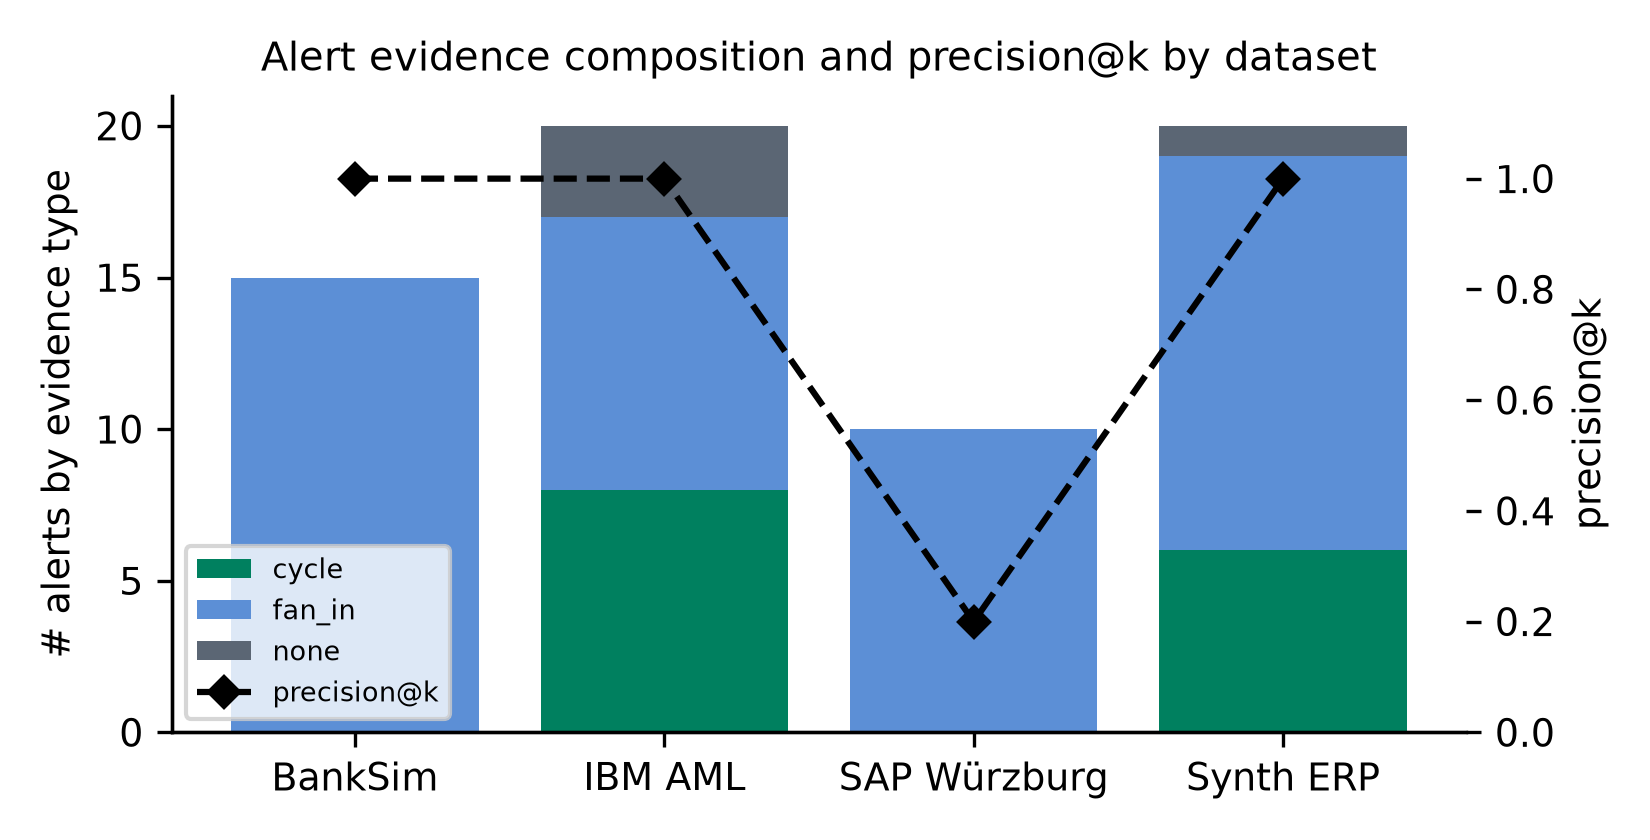
\includegraphics[width=\columnwidth]{figures/alert_evidence_mix.png}
\caption{Composition of graph evidence behind each dataset's top-$k$ alerts
(fan-in vs.\ cycle vs.\ no reconstructable structure), alongside precision@$k$.
Every bar sums to $k$ from Table~\ref{tab:alert_precision}.}
\label{fig:evidence_mix}
\end{figure}


\subsection{System: From Research Pipeline to Production Audit Console}\label{sec:system}\label{sec:production}

The preceding sections establish a narrow, defensible research claim about topology's marginal value under leakage-free evaluation. That claim is deliberately silent on whether the resulting models can run anywhere near a real ledger. Continuous-auditing research has long argued that a control is only as useful as the workflow that consumes it~\cite{vasarhelyi2012acceptance}, and post-implementation audits of ERP deployments routinely find that analytically sound models never reach production because the serving path, the data-integrity guarantees, and the operational evidence were never engineered~\cite{mamakou2024postimplementation}. This section describes what was actually built to close that gap: a Procure-to-Pay ERP core with a forensic audit console in front of it, an online scoring service that reuses the research pipeline's own feature-computation classes rather than reimplementing them, database-enforced financial-integrity invariants that do not trust application code to behave, and a measured (not assumed) performance and reliability profile. Every number in this section is either read directly from a project artifact file or drawn from a documented, reproducible test run; none are projected.

\subsubsection{Architecture Overview}\label{sec:system-arch}

The application is a conventional three-tier system chosen for auditability over novelty, consistent with the broader finding that ERP-adjacent ML systems succeed or fail on integration discipline more than on model sophistication~\cite{jawad2024erp}. A FastAPI backend exposes the ledger's domain objects (vendors, AP invoices, payments, payment runs, GL accounts, journal entries, audit alerts) through versioned REST routes (\texttt{app/api/\{vendors,invoices,payments,gl,alerts,auth,system\}.py}), backed by a normalized PostgreSQL schema and a Redis layer used for both response caching and idempotency-key bookkeeping. A React/TypeScript single-page frontend (\texttt{web/}) provides the clerk-facing ERP screens and the auditor-facing alert console. Neo4j sits alongside this stack strictly as a visualization and path-explanation surface for detected fraud alerts, never as a scoring dependency — the project's own methodology rules record that an earlier iteration let Neo4j silently become a load-bearing (and memory-exhausted) component of the scoring path, and this build deliberately keeps the database graph decorative.

The detail that distinguishes this system from a typical ML-in-the-loop web application is the scoring layer's relationship to the research code. \texttt{app.services.scoring\_service.FraudScoringService} does not reimplement the topology or tabular feature logic; it holds a live \texttt{OnlineTopologyState} and \texttt{OnlineOrdinaryState} per dataset/tenant, constructed directly from \texttt{topology.window\_graph.WindowGraph} and \texttt{topology.lap\_memory.LapMemory} — the exact classes \texttt{topology.engine.extract\_features} uses in the offline batch pipeline — plus a Welford-based incremental counterpart to the batch ordinary-feature builder. One instance is loaded per dataset at application startup from the persisted "online" bundle (\texttt{app/services/scoring\_registry.py}), and \texttt{/ready} reports honestly unavailable until at least one scoring service has loaded, rather than reporting healthy while silently unable to score. A single live ERP payment is routed to the \texttt{synth\_erp} scoring instance, the one dataset whose categorical vocabulary (\texttt{vendor\_payment}, \texttt{payroll}, \texttt{recurring\_bill}, \ldots) is a domain match for real AP postings.

%% FIGURE TODO: box-and-arrow diagram of the deployed system — ERP core (FastAPI + Postgres + Redis) on the left, the React audit console reading from it, the FraudScoringService holding live WindowGraph/LapMemory/Welford state on the right wired into the payment-posting path, Neo4j hanging off the alert console as visualization-only, and Prometheus/Grafana/Uptime Kuma scraping the API at the bottom — with a visual callout that the offline research pipeline (TGN training) is NOT in this runtime picture.
\begin{figure}[t]
  \centering
  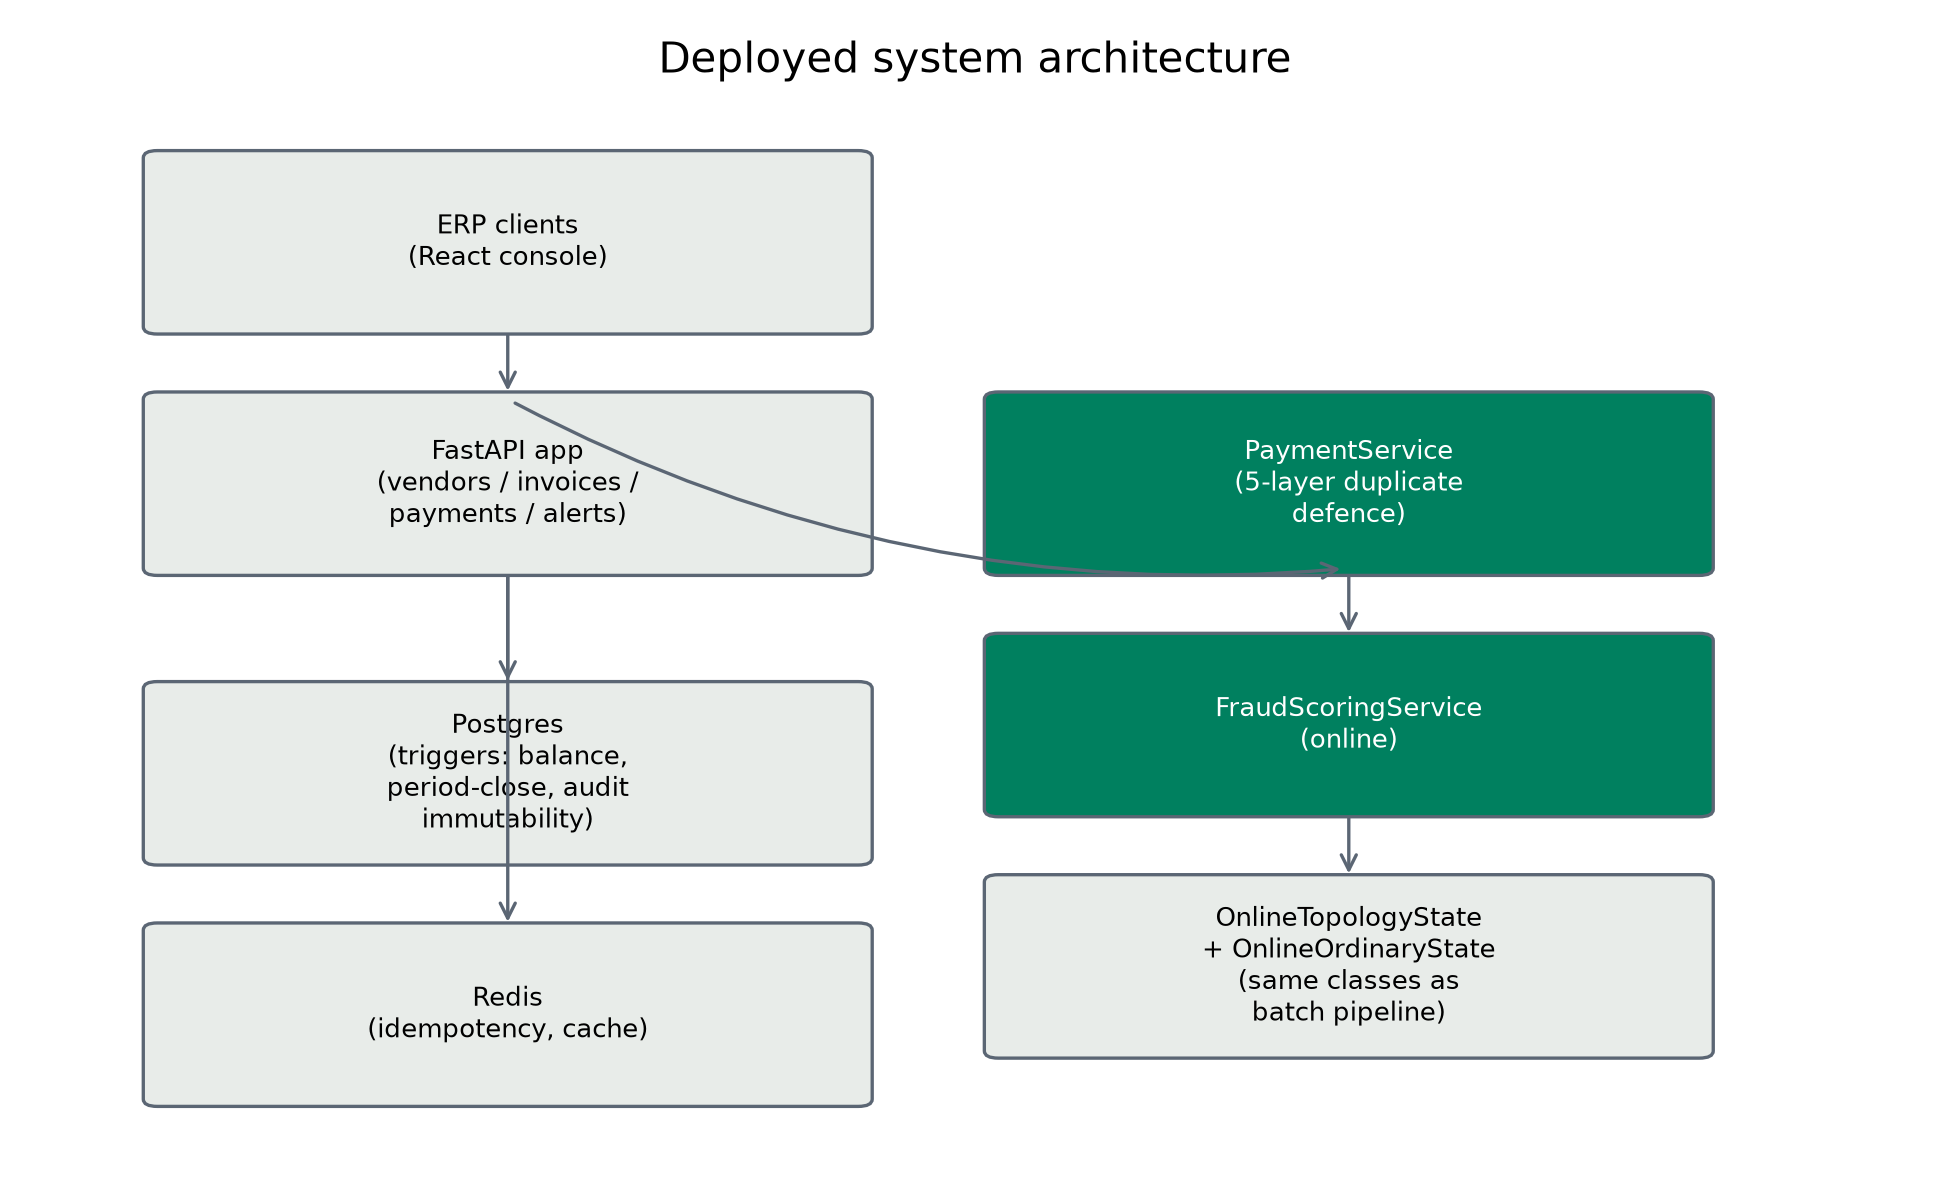
\includegraphics[width=\columnwidth]{figures/system_architecture.png}
  \caption{Deployed system architecture. The online \texttt{FraudScoringService} reuses the research pipeline's \texttt{WindowGraph}/\texttt{LapMemory} classes directly rather than a reimplementation; the offline TGN training path (Section~V) is not part of the serving runtime.}
  \label{fig:architecture}
\end{figure}

Correctness of the reuse, not merely its existence, is what makes the online path trustworthy: \texttt{tests/test\_online\_topology\_parity.py} replays 20{,}000 real transactions through both the batch \texttt{extract\_features} loop and \texttt{OnlineTopologyState.score\_transaction}, asserting every one of the thirteen topology feature columns matches exactly, row for row, with zero mismatches. The read-then-insert ordering inside the online class is copied line-for-line from the batch engine specifically to preserve this guarantee — the online driver differs only in holding one graph and two lap-memory instances alive across calls instead of discarding them after a single DataFrame pass.

\subsubsection{Financial Integrity as Database-Enforced Invariants}\label{sec:system-integrity}

An audit console is only as trustworthy as the ledger it reads from, and a recurring theme in ERP-integrity failures is that correctness logic lives entirely in application code that a bug, a bypassed service layer, or a future direct-SQL script can silently violate. This system treats three financial invariants as properties the database itself refuses to break, implemented as Postgres triggers (\texttt{alembic/versions/6192dae4f4a4\_gl\_invariants\_triggers.py}) rather than API-layer checks alone:

\begin{itemize}
  \item \textbf{Double-entry balance.} A \texttt{DEFERRABLE INITIALLY DEFERRED} constraint trigger on \texttt{journal\_lines} sums debits and credits per \texttt{journal\_entry\_id} and raises at \texttt{COMMIT}, not after each inserted line — necessary because a multi-line entry inserts its debit and credit rows separately and would fail a per-row check on every legitimate entry.
  \item \textbf{Period close.} An ordinary \texttt{BEFORE INSERT OR UPDATE} trigger on \texttt{journal\_entries} rejects any entry referencing a \texttt{fiscal\_period} whose status is not \texttt{open}. A FastAPI-level check exists purely to return a friendly \texttt{409} before the raw database exception would; the trigger is the actual enforcement.
  \item \textbf{Audit-log immutability.} \texttt{UPDATE} and \texttt{DELETE} on \texttt{audit\_log} are rejected outright by trigger, unconditionally. Only \texttt{INSERT} is a valid operation — the append-only property a SOX-style audit trail requires is a database guarantee here, not an application convention that a careless migration could quietly undermine.
\end{itemize}

Duplicate-payment prevention receives the same defense-in-depth treatment, layered so that no single control is trusted alone (\texttt{app/services/payment\_service.py}). An idempotency-key middleware replays the stored response for a retried request with the same key rather than re-executing it — the client-supplied-key pattern Helland~\cite{helland2012idempotence} argues is the only reliable way to make a mutating financial operation safe to retry, since the alternative (asking the caller never to retry, or de-duplicating on inferred request similarity) either fails under real network conditions or is not decidable in general. Independently, \texttt{create\_payment} takes a \texttt{SELECT ... FOR UPDATE} row lock on the target invoice \emph{before} checking for an existing active payment, closing the check-then-act race that two \emph{different} idempotency keys targeting the same invoice would otherwise open — the scenario a retry-only defense cannot cover, since it is two independent actors, not one repeated request. A partial unique index (\texttt{uq\_payments\_invoice\_live}, Module 3) is the database-level backstop if both application layers are ever bypassed. A \texttt{pg\_advisory\_xact\_lock} per vendor serializes an entire payment run, not just one invoice at a time. Finally, \texttt{tools/reconcile\_payments.py} is a periodic sweep that treats any invoice with more than one non-void payment as an incident — the tripwire for "we were wrong somewhere," not a preventive control. Table~\ref{tab:reliability} reports the formalized, automated test of this defense under real concurrency.


\section{Results and Analysis}\label{sec:results}

\subsection{Feature Importance, and a Result We Do Not Bury}\label{sec:engine-finding}

Table~\ref{tab:topology-importance} reports each topology feature's XGBoost
gain importance~\cite{chen2016xgboost}, normalized within the full
topology-augmented model (\texttt{topology\_full} arm) for each of the four
datasets carrying a complete ablation run. Because these thirteen columns
sit alongside 15--21 ordinary tabular features in that model (BankSim: 21
ordinary + 13 topology = 34; IBM AML: 8 + 13 = 21; SAP Würzburg: 20 + 13 =
33; synth\_erp: 15 + 13 = 28), the rows below do not sum to $1$ within a
dataset — the remaining gain mass sits with the ordinary features, not shown
here. SAP Würzburg's split sizes in this table (120{,}411 / 40{,}137 /
40{,}139, partition-aware by \texttt{run\_id}) come from
\texttt{ablation.json} specifically; the paper's headline champion-model
table elsewhere draws on a very slightly different SAP split
(120{,}341 / 40{,}114 / 40{,}116) recorded in \texttt{final\_champions.json} — the
two pipelines' SAP preprocessing diverged by 70 rows in the training split
and 23 rows in each of validation and test, and
the two are never mixed within one reported number.

\begin{table}[t]
\centering
\caption{Topology feature gain importance (fraction of total gain in the
topology-augmented model), by dataset. Source:
\texttt{paper/data/ablation.json}, \texttt{topology\_importance}, single
seed, no confidence intervals.}
\label{tab:topology-importance}
\resizebox{\columnwidth}{!}{%
\begin{tabular}{lrrrr}
\toprule
\textbf{Feature} & \textbf{BankSim} & \textbf{IBM AML} & \textbf{SAP Würzburg} & \textbf{synth\_erp} \\
\midrule
\texttt{in\_cycle}           & 0.0000 & 0.0000 & 0.0000 & 0.0040 \\
\texttt{cycle\_length}       & 0.0000 & 0.0009 & 0.0000 & 0.0029 \\
\texttt{in\_cycle\_ge3}      & 0.0000 & 0.0000 & 0.0000 & 0.0044 \\
\texttt{cycle\_amount\_ratio}& 0.0000 & 0.0008 & 0.0000 & 0.0090 \\
\texttt{cycle\_time\_span}   & 0.0000 & 0.0001 & 0.0000 & 0.0072 \\
\midrule
\texttt{fan\_in}             & 0.0908 & 0.0003 & 0.1791 & 0.0241 \\
\texttt{fan\_out}            & 0.0062 & 0.0010 & 0.0136 & 0.0189 \\
\texttt{dest\_in\_degree}    & 0.5199 & 0.0003 & 0.0682 & 0.0230 \\
\texttt{src\_out\_degree}    & 0.0062 & 0.0007 & 0.0089 & 0.0786 \\
\midrule
\texttt{lap\_in\_recur}      & 0.0052 & 0.0006 & 0.0319 & 0.0130 \\
\texttt{lap\_in\_payers}     & 0.0048 & 0.0006 & 0.0199 & 0.0103 \\
\texttt{lap\_out\_recur}     & 0.0066 & 0.5397 & 0.0416 & 0.0041 \\
\texttt{lap\_out\_payees}    & 0.0079 & 0.4200 & 0.0000 & 0.0036 \\
\bottomrule
\end{tabular}%
}
\end{table}

%% FIGURE TODO: grouped bar chart, one panel per dataset (BankSim, IBM AML,
%% SAP Würzburg, synth_erp), bars = gain importance for the 13 topology
%% features colour-coded by group (cycle / degree-fan / lapping), y-axis
%% shared across panels to make visually obvious that the 5 cycle-feature
%% bars are flat at zero in 3 of the 4 panels and barely visible in the 4th.
\begin{figure}[t]
\centering
% \includegraphics[width=\columnwidth]{figures/topology_importance_by_group.png}
\caption{Gain importance of the thirteen topology features, grouped by
detector family and faceted by dataset. Cycle-detector bars (leftmost group
in each panel) are at or indistinguishable from zero in three of four
datasets.}
\label{fig:cycle-null}
\end{figure}

The pattern the table makes plain is not subtle, and we state it without
qualification: the five cycle features — \texttt{in\_cycle},
\texttt{cycle\_length}, \texttt{in\_cycle\_ge3}, \texttt{cycle\_amount\_ratio},
\texttt{cycle\_time\_span} — carry essentially zero gain importance on three
of the four datasets. On BankSim and SAP Würzburg every one of the five is
exactly $0.0000$; on IBM AML the largest is \texttt{cycle\_length} at
$0.0009$, well over two orders of magnitude below that dataset's dominant features
(\texttt{lap\_out\_recur} $0.5397$, \texttt{lap\_out\_payees} $0.4200$). Only
on \texttt{synth\_erp} — our own generated dataset, used for
training/stress-testing and never as headline proof — do cycle features
carry non-trivial weight, and even there the largest single one
(\texttt{cycle\_amount\_ratio}, $0.0090$) is under one percent of total gain.
This is a pointed result for a project whose title is built around a
"shadow ledger" of detected cycles: the cycle detector is not inert by
construction (\S\ref{sec:engine-windowgraph} shows it is a real, bounded BFS
that fires and populates non-\texttt{NaN} values whenever a loop closes,
and it is validated separately against IBM AML's labeled ground-truth cycles
in the ablation study), yet the boosted-tree model consistently prefers
other signals to explain fraud once they are available. IBM AML is the most
striking case, because it is precisely the dataset engineered with labeled
cycle-shaped fraud~\cite{altman2023realistic} — and it is exactly where
cycle-feature gain is most thoroughly crowded out: \texttt{lap\_out\_recur}
and \texttt{lap\_out\_payees} alone account for gain fraction $0.9597$ out of
the full 21-feature model's normalized total of $1.0$ — the two amount-derived
lapping features claim $96\%$ of \emph{every} split the model makes, ordinary
tabular features included, leaving essentially nothing for the five cycle
columns.
Our working hypothesis, developed fully where the predictive consequences of
this pattern are analyzed, is two-part: true cycles are rare enough in every
dataset we could build (a handful of closures against hundreds of thousands
of transactions) that a gradient-boosted tree finds little marginal
information in them once even coarser degree/fan and amount-recurrence
signals are on the table, and where a cycle transaction and an
amount-lapping signature co-occur, the amount/lapping features are simply
more discriminative per split — so the tree spends its gain budget there
first and has little left to reward on the rarer cycle columns. We do not
claim this hypothesis is proven by Table~\ref{tab:topology-importance} alone;
it is a description of what the importances show, offered as the
starting point the ablation study's marginal-lift and amount-blind results
either support or complicate.

\subsection{The Ablation: Results Across Four Datasets}\label{sec:ablation}
Table~\ref{tab:ablation-arms} reports test-split PR-AUC for all seven arms on all four datasets, read directly from \texttt{ablation.json}. Table~\ref{tab:ablation-lifts} reports the four lift statistics derived from it. Both are single-seed (seed 42) results; the statistical status of these numbers is addressed explicitly in \S\ref{sec:ablation-stats} before any of them are interpreted causally.

\begin{table}[t]
\centering
\caption{Test-split PR-AUC (average precision) across the seven ablation arms, by dataset. B = ordinary baseline; T = all topology (incl.\ amount-derived); S = pure structure only (8 of 13 topology features); subscript $\neg a$ = amount columns removed from the ordinary set. Single seed (42); \texttt{paper/data/ablation.json}.}
\label{tab:ablation-arms}
\small
\begin{tabular}{lcccc}
\toprule
Arm & BankSim & IBM AML & SAP W. & Synth-ERP \\
\midrule
B & 0.833 & 0.990 & 0.155 & 0.163 \\
B+T & 0.931 & 1.000 & 0.046 & 0.563 \\
B+S & 0.930 & 0.998 & 0.072 & 0.566 \\
B$_{\neg a}$ & 0.634 & 0.093 & 0.049 & 0.157 \\
B$_{\neg a}$+T & 0.822 & 0.867 & 0.055 & 0.503 \\
B$_{\neg a}$+S \emph{(clean)} & 0.824 & 0.184 & 0.064 & 0.269 \\
T-only & 0.483 & 0.633 & 0.024 & 0.306 \\
\bottomrule
\end{tabular}
\end{table}

\begin{table}[t]
\centering
\caption{The four ablation lift statistics (test-split PR-AUC deltas). Positive = helps; negative = hurts. \texttt{paper/data/ablation.json}.}
\label{tab:ablation-lifts}
\small
\resizebox{\columnwidth}{!}{%
\begin{tabular}{lcccc}
\toprule
Dataset & $\Delta$Topo (full) & $\Delta$Struct (full) & $\Delta$Topo (blind) & $\Delta$Struct (blind, clean) \\
\midrule
BankSim & +0.0977 & +0.0974 & +0.1883 & +0.1899 \\
IBM AML & +0.0100 & +0.0079 & +0.7735 & +0.0905 \\
SAP W. & $-$0.1090 & $-$0.0829 & +0.0056 & +0.0153 \\
Synth-ERP & +0.4000 & +0.4031 & +0.3451 & +0.1115 \\
\bottomrule
\end{tabular}}
\end{table}

%% FIGURE TODO: grouped bar chart, one group per dataset (BankSim, IBM AML, SAP Wurzburg, Synth-ERP), four bars per group showing the four lift statistics from Table 2 (marginal-topology, marginal-structure, amount-blind-topology, amount-blind-structure), with a zero line and SAP Wurzburg's two negative bars visually distinct (e.g. hatched/red) from the three positive datasets.
\begin{figure}[t]
\centering
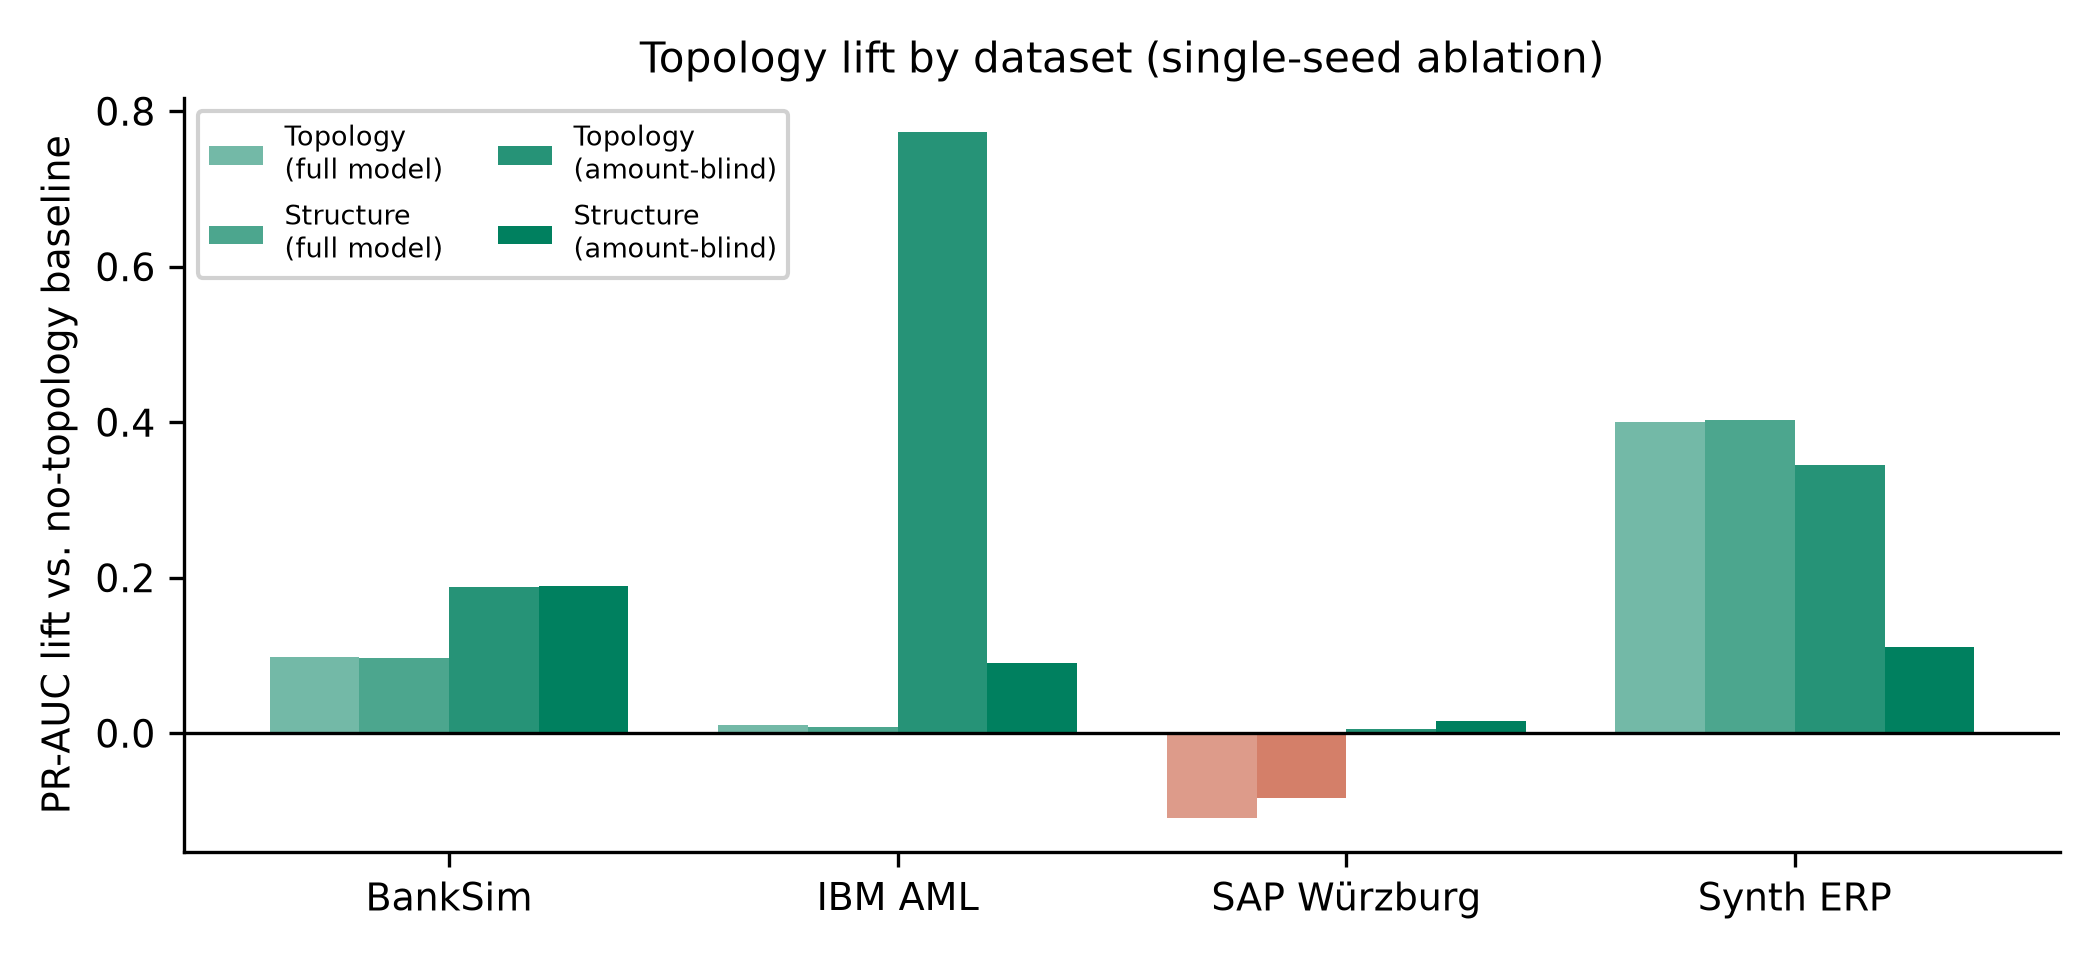
\includegraphics[width=\columnwidth]{figures/ablation_lift_by_dataset.png}
\caption{The four lift statistics of Table~\ref{tab:ablation-lifts} plotted by dataset, making visually explicit that SAP W\"urzburg is the only dataset where both full-model lifts are negative while its two amount-blind lifts remain (barely) positive.}
\label{fig:ablation-lift-by-dataset}
\end{figure}

\subsubsection{Dataset-by-dataset verdict}
\textbf{BankSim: yes.} The full-model structure lift is $+0.0974$ PR-AUC (an $11.7\%$ relative improvement over the $0.833$ baseline, $0.0974/0.833$), and — decisively — the clean amount-blind probe confirms it independently: with every amount feature removed from both sides of the comparison, pure structure still adds $+0.1899$ PR-AUC ($0.634 \to 0.824$). BankSim's topology-importance breakdown (\texttt{ablation.json}) attributes this almost entirely to two density features, \texttt{dest\_in\_degree} (gain importance $0.520$) and \texttt{fan\_in} ($0.091$): BankSim transactions run customer $\to$ merchant, so cycles are structurally impossible, and the signal that remains is exactly the "many senders funnel into one receiver" mule-collection pattern the fan-in features are built to detect. This is the cleanest positive result in the ablation, on a real (simulated-but-not-synthetic-generated) dataset, under both the contaminated and the clean test.

\textbf{IBM~AML: uninformative in the full model; the real signal is elsewhere.} The ordinary baseline alone already reaches PR-AUC $0.990$, leaving essentially no headroom: the full-model structure lift of $+0.0079$ is small in both absolute and relative terms, and — as \S\ref{sec:ablation-stats} makes explicit — falls below this project's own single-seed noise floor, so it cannot be read as evidence of anything. The dirty amount-blind topology probe reaches a striking PR-AUC of $0.867$ ($+0.7735$ lift over the amount-blind baseline's $0.093$), but this number is not evidence for structure: \texttt{topology\_importance} shows \texttt{lap\_out\_recur} ($0.540$) and \texttt{lap\_out\_payees} ($0.420$) together account for $96\%$ of the gain inside that arm, and both are the amount-derived lapping features excluded from the pure-structure set. The clean amount-blind structure probe — the only honest version of this test — reaches PR-AUC $0.184$, a lift of $+0.0905$ over the $0.093$ amount-blind baseline: real, but an order of magnitude smaller than the $0.867$ figure a less careful ablation would have reported as "topology's contribution." In short: IBM~AML's frauds are given away by recurring near-equal amounts (a re-encoded amount signal, not a graph shape), a finding this project's own earlier probing flagged as refuting its initial premise that IBM~AML would be the decisive topology testbed.

\textbf{SAP W\"urzburg: no — topology actively hurts.} Both full-model lifts are negative: $-0.1090$ for all topology, $-0.0829$ for pure structure alone (\texttt{marginal\_structure\_lift = -0.08288}, the number this project's own methodology rules single out as never to be softened or omitted). Adding any topology columns to the ordinary baseline drives test PR-AUC down from $0.155$ to $0.072$ (structure) or $0.046$ (all topology) — a genuinely negative result, not merely a null one. The two amount-blind lifts are small and positive ($+0.0056$, $+0.0153$), but both baselines they are measured against are themselves extremely weak (PR-AUC $0.049$), so this offers no rehabilitation. SAP W\"urzburg is also the one dataset in this study with only $25$ test-split frauds, which we treat as a hard interpretability ceiling rather than a footnote: with that few positive examples, a handful of ranking swaps can move PR-AUC by tens of a point, and \S\ref{sec:ablation-stats} presents an independent, multi-seed confirmation that this dataset's metrics are indeed unstable. We report the negative result plainly rather than either suppressing it or explaining it away, while being explicit that "topology hurts here" and "this measurement is high-variance" are both true simultaneously.

\textbf{Synth-ERP: yes, the largest lift measured — and the one result that cannot be used as thesis evidence.} The full-model structure lift is $+0.4031$ PR-AUC, a $246.8\%$ relative improvement over a weak $0.163$ baseline, with a clean amount-blind confirmation of $+0.1115$. This is real signal by every measure this ablation applies. It is also, definitionally, the least informative result for the paper's actual scientific claim: synth\_erp is this project's own generated dataset, built and calibrated specifically to have rich, ERP-flavored graph structure, and the project's binding policy (adopted precisely to avoid grading its own homework) treats it as a training/stress-testing corpus only, never as evidence that topology helps on real transaction data. We report the number because it is honest and instructive about what topology \emph{can} do when a dataset is constructed to contain strong structural fraud signatures — but it answers a different, narrower question than the one this section opened with.

\subsubsection{Statistical caveats: one seed, no confidence intervals, and a stated noise floor}\label{sec:ablation-stats}
Every number in Tables~\ref{tab:ablation-arms} and \ref{tab:ablation-lifts} comes from a single training run per arm (seed 42), not an average over repeated runs. \texttt{ablation.json} carries no standard deviations, no confidence intervals, and no significance tests, and none should be inferred from it. This project's own training harness documents its rationale for treating small single-seed margins with suspicion: per the comment in \texttt{src/modeling/harness.py}, "single-seed differences of $\sim$0.01 PR-AUC are within XGBoost's subsample noise," and \texttt{experiments/ablation.py}'s own verdict logic uses exactly this $0.01$ figure as the cutoff below which a lift is characterized as "adds $\sim$nothing" rather than a genuine effect. By this project's own stated standard, IBM~AML's full-model structure lift of $+0.00792$ is below the noise floor and is not distinguishable from zero on the evidence of a single seed — a second, independent reason (beyond baseline saturation) that the IBM~AML full-model comparison cannot be read as informative.

A separate, multi-seed experiment offers some corroborating context, though it is not a like-for-like repetition of the arms above: \texttt{final\_champions.json} trains each dataset's final champion configuration — ordinary $+$ topology $+$ TGN embeddings, a superset of the ablation's \emph{+Structure} arm that additionally includes the 65-dimensional temporal-graph-network features discussed elsewhere in this paper — three times, with seeds $\{42,43,44\}$, and reports mean $\pm$ standard deviation. Its per-dataset stability is informative about exactly the concern raised above: BankSim's three-seed test PR-AUC is $0.9364 \pm 0.0015$ (a $0.16\%$ relative standard deviation), consistent with this dataset's ranking being robust to seed choice; SAP W\"urzburg's is $0.1557 \pm 0.0717$ — a $46\%$ relative standard deviation on the mean — which independently corroborates, from a completely different experiment and feature set, the instability that the ablation's own 25-test-fraud caveat already predicts. SAP W\"urzburg's imbalance-mechanism selection for this same champion run is explicitly flagged \texttt{reliable:~false}, and its hyperparameter search was skipped altogether (validation frauds below the guard threshold described in \S\ref{sec:protocol}), so its champion runs on the harness's locked default configuration rather than a tuned one. None of this changes the ablation's central negative finding for SAP W\"urzburg — if anything it strengthens the case for treating that finding as directionally real but numerically imprecise, exactly as reported above — but it is a materially different, TGN-inclusive experiment and its numbers should not be conflated with the seed-42-only ablation arms in Tables~\ref{tab:ablation-arms}--\ref{tab:ablation-lifts}. We also note, to keep every PR-AUC in this paper unambiguous: the champion figures cited in this paragraph describe the offline, research-only model family evaluated for this ablation and are not the model served by the production audit console, which for latency and reproducibility reasons excludes the TGN component; that distinction is maintained precisely wherever this paper reports a PR-AUC for a specific model.

\subsubsection{The cycle-feature paradox}
The project's topology engine was built around five detectors intended to be its signature contribution — \texttt{in\_cycle}, \texttt{cycle\_length}, \texttt{in\_cycle\_ge3}, \texttt{cycle\_amount\_ratio}, and \texttt{cycle\_time\_span} — measuring whether a transaction closes a money loop, how long that loop is, and how tightly it conserves the amount that entered it. The ablation's own gain-importance breakdown does not support these as the load-bearing signal. Table~\ref{tab:cycle-importance} sums the gain importance of all five cycle features, within the full \emph{+Topology} model, against the single highest-importance density feature on the same dataset. On three of the four datasets — BankSim, IBM~AML, and SAP W\"urzburg — every one of the five cycle features scores exactly $0.0$ gain importance; the model finds no split in five hundred boosting rounds for which distinguishing "closes a 3-hop cycle" from "does not" reduces loss more than an already-available split on in-degree, fan-in, or (on IBM~AML) the amount-derived lapping columns. Only on synth\_erp — the one dataset engineered specifically to contain rich cyclic laundering structure — do the cycle features register non-zero importance, and even there their combined mass ($0.0275$) is roughly a third of the single top feature, \texttt{src\_out\_degree} ($0.0786$).

\begin{table}[t]
\centering
\caption{Combined gain importance of the five cycle features vs.\ the single highest-importance density feature, within the baseline+topology model. \texttt{topology\_importance}, \texttt{paper/data/ablation.json}.}
\label{tab:cycle-importance}
\small
\begin{tabular}{lccc}
\toprule
Dataset & $\Sigma$ cycle feats. & Top non-cycle feat. & Importance \\
\midrule
BankSim & 0.0000 & \texttt{dest\_in\_degree} & 0.5199 \\
IBM AML & 0.0018 & \texttt{lap\_out\_recur}$^\dagger$ & 0.5397 \\
SAP W. & 0.0000 & \texttt{fan\_in} & 0.1791 \\
Synth-ERP & 0.0275 & \texttt{src\_out\_degree} & 0.0786 \\
\bottomrule
\end{tabular}
\\[3pt]
\raggedright{\scriptsize $^\dagger$Amount-derived, not pure structure. Among pure-structure features on IBM AML, the top scorer is \texttt{dest\_in\_degree}/\texttt{fan\_in} at $0.0003$.}
\end{table}

%% FIGURE TODO: small-multiples heatmap, one panel per dataset, rows = the 13 topology feature names (grouped visually into the 8 pure-structure and 5 amount-derived features), single column of cell shading by gain importance value from topology_importance in ablation.json, making the "cycle features are a near-empty column on 3 of 4 panels" pattern visible at a glance.
\begin{figure}[t]
\centering
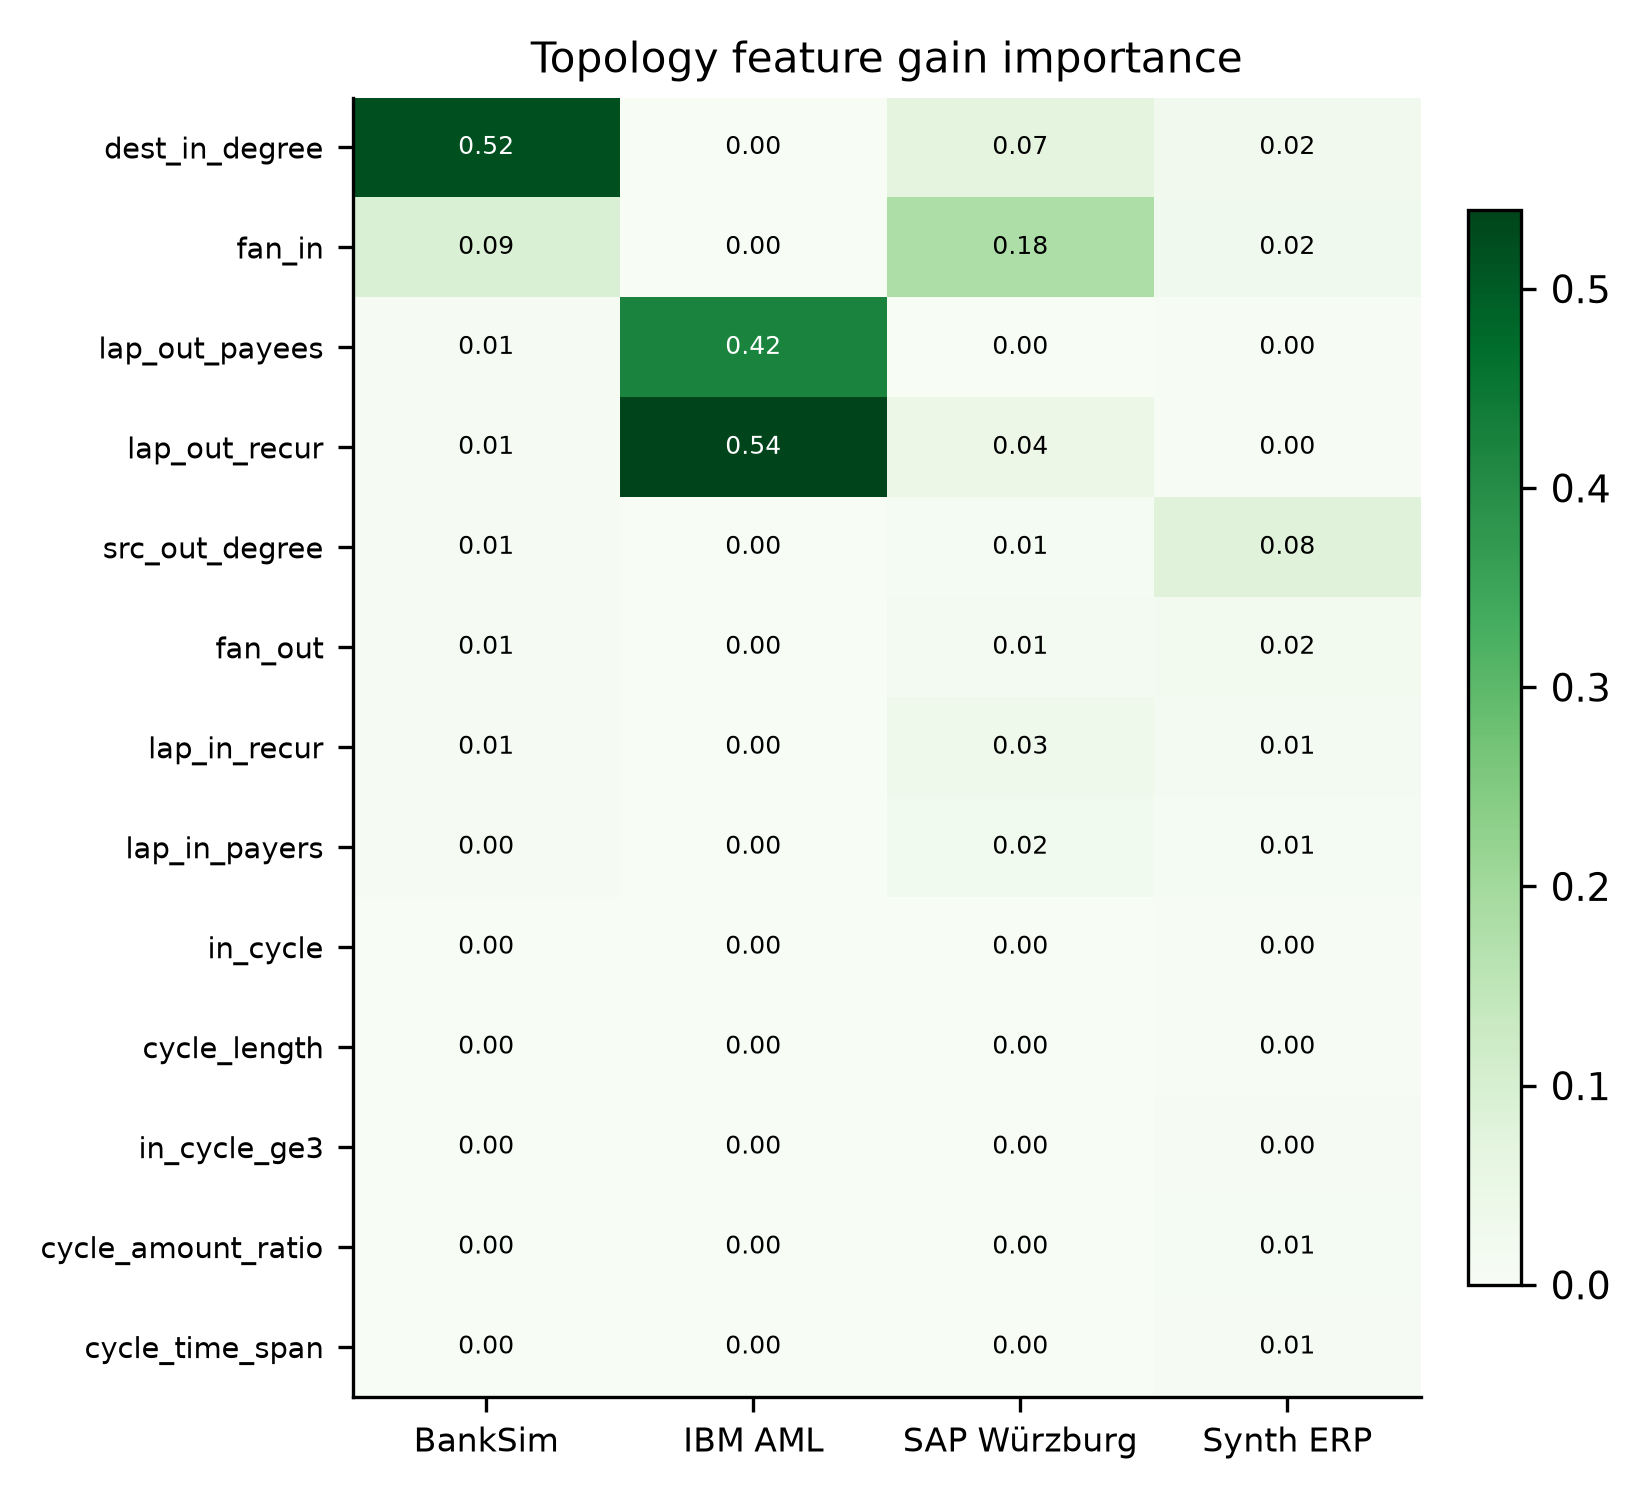
\includegraphics[width=\columnwidth]{figures/topology_importance_heatmap.png}
\caption{Topology feature gain importance by dataset (\texttt{topology\_importance}, Table~\ref{tab:cycle-importance}'s underlying data), grouping pure-structure against amount-derived features and making visible how consistently the five cycle features sit at or near zero while a small number of density features (in-degree, fan-in) or amount-derived lapping features carry essentially all of the mass.}
\label{fig:cycle-heatmap}
\end{figure}


\subsection{Modernization: Focal Loss and Temporal Graph Networks}\label{sec:modern}

The ablation study above establishes, from a single training seed, that hand-crafted topology features carry a leakage-free signal on BankSim and (conditionally) on IBM AML. Two questions remain unanswered by a single seed: whether that signal is robust to run-to-run randomness, and whether a \emph{learned} structural representation --- one that does not depend on the five hand-designed detectors --- can do better. This section reports a second, purpose-built study that answers both. Every arm below is trained with three random seeds (42, 43, 44) and reported as mean $\pm$ standard deviation, the project's own minimum bar for treating a difference as real rather than noise. Two independent upgrades to the locked XGBoost baseline are tested: (1) focal loss~\cite{lin2017focal} as an alternative to class-weighting for handling the $<$1.3\% fraud rate, implemented as a custom, deliberately alpha-free XGBoost~\cite{chen2016xgboost} objective so that it never doubles up with class weights as a second imbalance mechanism; and (2) a Temporal Graph Network (TGN)~\cite{rossi2020temporal}, a self-supervised, label-free encoder that learns a 32-dimensional GRU memory vector per account from the raw transaction stream and emits it, frozen, as 65 additional feature columns (32 source-account dimensions, 32 destination-account dimensions, and one scalar ``edge-expectedness'' score summarizing how surprising the pair is given the account's history). Because it is trained purely as next-link prediction, TGN sees no fraud labels and, following the project's own lapping-detector lesson, is deliberately amount-blind: it observes only who transacted with whom and when.

All results in this section come from \texttt{paper/data/modern.json} (the controlled multi-seed comparison) and \texttt{paper/data/final\_champions.json} (the actual champion-selection pipeline, which additionally runs a light 20-configuration hyperparameter search); numbers drawn from the single-seed ablation study are marked explicitly as such. Four feature-family arms are compared, holding the time-aware splits, XGBoost hyperparameters and (where noted) imbalance mechanism fixed within each comparison: \textbf{A} = ordinary transaction features only (21/8/20/15 features for BankSim/IBM~AML/SAP~Würzburg/synth\_erp); \textbf{B} = A + the 13 hand-crafted topology features; \textbf{C} = A + the 65 TGN columns (no hand-crafted topology); \textbf{D} = A + topology + TGN combined. The 13-feature topology block and 65-feature TGN block are identical in width across all four datasets, which is a useful internal consistency check: $|A|+13+65$ equals the reported full-feature-set size in every case (e.g.\ $21+13+65=99$ for BankSim, $8+13+65=86$ for IBM~AML). The focal-vs-class-weight comparison is run on arms A and B only (both imbalance mechanisms); arms C and D are run with class weights alone, since their purpose is to isolate the marginal value of a learned structural representation, not to re-litigate the imbalance-mechanism question a second time.

One dataset-scope note carries over from the ablation study: SAP Würzburg's splits in this section (120{,}341 / 40{,}114 / 40{,}116 train/val/test, 204/19/25 frauds, taken from \texttt{modern.json} and matching \texttt{final\_champions.json}) are the non-partition-aware split, not the partition-aware split (120{,}411 / 40{,}137 / 40{,}139) used elsewhere in this paper's headline ablation; the two SAP Würzburg number sets should not be pooled.

\subsubsection{Focal loss versus class weights}

Table~\ref{tab:focal-arms} reports the three-seed test PR-AUC for the ordinary-only (A) and ordinary+topology (B) arms under both imbalance mechanisms. Focal loss helps on the ordinary-only baseline in all four datasets, most dramatically on SAP Würzburg (+0.0383) and synth\_erp (+0.1690); once topology is added, its effect is mixed --- a small loss on BankSim ($-0.0060$), a wash on IBM AML (0.0000, both already at the PR-AUC ceiling), a large and volatile gain on SAP Würzburg (+0.2460, on 25 test frauds), and a solid gain on synth\_erp (+0.2014).

\begin{table}[t]
\centering
\caption{Three-seed test PR-AUC, class weights vs.\ focal loss ($\gamma{=}2.0$), ordinary-only (A) and ordinary+topology (B) arms. $\Delta$ = focal $-$ class-weight. $^\dagger$synth\_erp is synthetic and never used as thesis evidence.}
\label{tab:focal-arms}
\resizebox{\columnwidth}{!}{%
\scriptsize
\begin{tabular}{lrrrrrr}
\toprule
Dataset & A$_{cw}$ & A$_{focal}$ & $\Delta_A$ & B$_{cw}$ & B$_{focal}$ & $\Delta_B$ \\
\midrule
BankSim & 0.7870{\tiny$\pm$0.0700} & 0.8616{\tiny$\pm$0.0001} & +0.0746 & 0.9319{\tiny$\pm$0.0017} & 0.9259{\tiny$\pm$0.0008} & $-$0.0060 \\
IBM AML & 0.9920{\tiny$\pm$0.0026} & 0.9968{\tiny$\pm$0.0001} & +0.0048 & 1.0000{\tiny$\pm$0.0000} & 1.0000{\tiny$\pm$0.0000} & 0.0000 \\
SAP Würzburg & 0.1581{\tiny$\pm$0.0129} & 0.1963{\tiny$\pm$0.0252} & +0.0383 & 0.0717{\tiny$\pm$0.0095} & 0.3177{\tiny$\pm$0.1470} & +0.2460 \\
synth\_erp$^\dagger$ & 0.2483{\tiny$\pm$0.0602} & 0.4173{\tiny$\pm$0.0120} & +0.1690 & 0.4569{\tiny$\pm$0.1547} & 0.6583{\tiny$\pm$0.0031} & +0.2014 \\
\bottomrule
\end{tabular}}
\end{table}

The most consequential effect of focal loss, however, is not its mean shift but its effect on \emph{variance}. On BankSim's ordinary-only arm, moving from class weights to focal loss collapses the three-seed standard deviation from 0.0700 to 0.00007 --- roughly three orders of magnitude, from ``a coin-flip's width of uncertainty'' to ``machine-precision-adjacent.'' This is sharpened by comparing against the single-seed ablation study, which reported a BankSim baseline PR-AUC of 0.8330 (\texttt{ablation.json}, seed 42 only, class weights). That single number sits roughly two-thirds of one standard deviation above the three-seed class-weight mean of 0.7870 reported here --- a concrete illustration of why the project's own methodology treats single-seed differences smaller than $\sim$0.01 PR-AUC as noise: an unlucky or lucky seed choice alone can move the class-weighted BankSim baseline by several hundredths. Under focal loss the same arm's three-seed spread (0.8616 $\pm$ 0.00007) makes this kind of seed sensitivity essentially disappear.

This variance-collapsing property is also what wins focal loss its place in the champion pipeline. Table~\ref{tab:champion-selection} reports \texttt{final\_champions.json}'s validation-selection step, which compares the full feature set (A+B+C combined, i.e.\ arm D) under class weights against the same feature set under focal loss and selects whichever wins on validation PR-AUC --- never on test. Focal loss wins the selection on three of the four datasets: BankSim, SAP Würzburg, and synth\_erp; on IBM AML the two mechanisms tie exactly at the saturated ceiling (1.0000 vs.\ 1.0000) and the pipeline's tie-break falls to class weights. Note that this selection step differs from the controlled arm-D comparison in that it also runs a 20-configuration hyperparameter search per candidate (skipped only for SAP Würzburg, whose validation fraud count trips the pipeline's own small-sample guard), so its validation numbers are close to, but not identical with, the fixed-hyperparameter arm-D numbers reported elsewhere in this section --- for example BankSim's tuned class-weight validation PR-AUC is 0.9489 versus the fixed-hyperparameter arm D's 0.9426.

\begin{table}[t]
\centering
\caption{Champion validation selection (\texttt{final\_champions.json}), full feature set (topology+TGN+ordinary). Margin = focal $-$ class-weight on validation. $^\ddagger$selection flagged \texttt{reliable=false} (SAP Würzburg's HPO was skipped by the small-sample guard). $^\dagger$synth\_erp is non-evidentiary.}
\label{tab:champion-selection}
\resizebox{\columnwidth}{!}{%
\scriptsize
\begin{tabular}{lrrlrr}
\toprule
Dataset & Val (cw) & Val (focal) & Winner (margin) & Test (cw) & Test (focal) \\
\midrule
BankSim & 0.9489{\tiny$\pm$0.0009} & 0.9515{\tiny$\pm$0.0007} & focal (+0.0026) & 0.9395{\tiny$\pm$0.0006} & 0.9364{\tiny$\pm$0.0015} \\
IBM AML & 1.0000{\tiny$\pm$0.0000} & 1.0000{\tiny$\pm$0.0000} & cw (tie, 0.0000) & 1.0000{\tiny$\pm$0.0000} & 1.0000{\tiny$\pm$0.0000} \\
SAP Würzburg & 0.2888{\tiny$\pm$0.0436} & 0.3562{\tiny$\pm$0.0195} & focal$^\ddagger$ (+0.0674) & 0.1401{\tiny$\pm$0.0076} & 0.1557{\tiny$\pm$0.0717} \\
synth\_erp$^\dagger$ & 0.8487{\tiny$\pm$0.0017} & 0.8507{\tiny$\pm$0.0025} & focal (+0.0020) & 0.7722{\tiny$\pm$0.0014} & 0.7785{\tiny$\pm$0.0053} \\
\bottomrule
\end{tabular}}
\end{table}

BankSim deserves a specific flag: its validation margin, +0.0026 PR-AUC, is the thinnest \emph{reliable, non-saturated, real-data} margin in the entire selection table --- synth\_erp's nominal margin (+0.0020) is numerically smaller but is excluded from thesis claims as synthetic data, and IBM AML's margin is a literal zero-width tie on an already-saturated metric, not a genuine comparison. A margin this thin, on the dataset the project treats as its cleanest structural-signal testbed, does not survive contact with the test set: the class-weight arm actually scores higher on BankSim's held-out test period (0.9395 $\pm$ 0.0006) than the focal arm that was selected on validation (0.9364 $\pm$ 0.0015), a reversal of 0.0032 PR-AUC. We report this plainly as a caution against over-reading small validation margins, per the project's own threshold-freezing discipline; it does not overturn the selection (validation-only selection is the whole point of never touching test until after the choice is frozen), and it is operationally invisible at the metric an auditor actually cares about --- precision@100 is 1.00 for both arms.

\subsubsection{Temporal graph network embeddings}

Table~\ref{tab:tgn-lift} isolates the value of the learned TGN representation against two references: the ordinary-only baseline (arm C $-$ arm A, both class-weighted) and the hand-crafted topology block (arm C $-$ arm B), plus the incremental value of combining both representations (arm D $-$ arm B) and TGN's share of total SHAP feature importance in the champion model (from \texttt{final\_champions.json}'s per-dataset SHAP summary).

\begin{table}[t]
\centering
\caption{TGN embeddings vs.\ hand-crafted topology, 3-seed test PR-AUC deltas (class-weighted arms only) and TGN's share of total SHAP importance in the champion model. $^\dagger$synth\_erp is non-evidentiary.}
\label{tab:tgn-lift}
\resizebox{\columnwidth}{!}{%
\scriptsize
\begin{tabular}{lrrrr}
\toprule
Dataset & TGN$-$base. & TGN$-$topo. & Comb.$-$topo. & TGN SHAP share \\
\midrule
BankSim & +0.1326 & $-$0.0123 & +0.0004 & 17.5\% \\
IBM AML & $-$0.0048 & $-$0.0128 & 0.0000 & 1.9\% \\
SAP Würzburg & $-$0.0987 & $-$0.0124 & +0.0684 & 42.0\% \\
synth\_erp$^\dagger$ & +0.4489 & +0.2404 & +0.2850 & 37.3\% \\
\bottomrule
\end{tabular}}
\end{table}

The central, load-bearing finding of this table is the middle column. On every real dataset, TGN alone (arm C) scores \emph{below} hand-crafted topology alone (arm B): $-$0.0123 on BankSim, $-$0.0128 on IBM AML, $-$0.0124 on SAP Würzburg. These three deltas are remarkably tight given how different the three datasets are in scale, fraud rate, and graph density --- all three cluster within 0.0005 of $-$0.0125. Learned, self-supervised structural embeddings simply do not beat five purpose-built, domain-informed detectors on real transaction graphs in this study; the only dataset where TGN outperforms hand-crafted topology is synth\_erp (+0.2404), the project's own synthetic environment, which is explicitly excluded from evidentiary claims (Section~\ref{sec:threats}). The first column tells a related but distinct story: TGN's lift over the plain ordinary-feature baseline is positive on BankSim (+0.1326, nearly matching topology's own +0.1449 lift there) but slightly \emph{negative} on both IBM AML ($-$0.0048) and SAP Würzburg ($-$0.0987). On IBM AML this is a small movement within noise (both arms sit near the saturated ceiling, std $\approx$0.01); on SAP Würzburg it is a large, consistent penalty, echoing the same dataset's negative topology lift reported in the ablation study --- on this small, thin ERP ledger, adding structural feature complexity of either kind tends to hurt rather than help, plausibly because 25 test frauds cannot support the additional degrees of freedom either representation introduces.

Combining topology and TGN (arm D vs.\ arm B) adds negligible value beyond topology alone on the two datasets with the cleanest signal: +0.0004 on BankSim, 0.0000 on IBM AML (already saturated). SAP Würzburg's combined arm does show a nominal +0.0684 recovery over its topology-only arm, but this sits inside the same small-sample volatility that produced SAP's other large, sign-flipping deltas in this section and should not be read as evidence that TGN rescues topology's failure there. synth\_erp's large combined gain (+0.2850) is, again, a synthetic-data result only.

This pattern is consistent with, not contradicted by, the 2026 literature on graph-native alternatives: Lei et al.'s STC-MixHop~\cite{lei2026stcmixhop} reports the same qualitative result on a different transaction-fraud benchmark, that a graph-learning architecture struggles to outperform a tabular baseline once node attributes already carry strong signal, and attributes graph structure's value specifically to settings where relational patterns are operationally significant rather than universal. This paper's own dataset-by-dataset TGN comparison is, in effect, an independent empirical instance of exactly that claim: TGN loses to hand-crafted topology on every real dataset in this study, each of which differs in scale, fraud rate, and graph density, and wins only on the one dataset (\texttt{synth\_erp}) explicitly engineered to have rich, easily learnable structure.

A last observation cautions against reading SHAP importance share as a proxy for ablation-validated value. SAP Würzburg's TGN block claims the \emph{largest} share of total SHAP importance of any dataset in this study (42.0\%) despite producing the study's most negative TGN lift ($-$0.0987 over baseline, $-$0.0124 over topology); IBM AML shows the opposite pattern, with TGN carrying almost no importance (1.9\%) on a baseline it also fails to improve. A feature family can dominate a model's internal attribution and still not earn its place in a leakage-free ablation --- the same lesson the ablation study draws for hand-crafted cycle features applies here to a learned representation as well, via TreeSHAP's exact per-feature attribution~\cite{lundberg2017unified,lundberg2020local}.

%% FIGURE TODO: grouped bar chart, one group per dataset (BankSim, IBM AML, SAP Würzburg, synth_erp), two bars per group showing tgn_vs_handcrafted_topology and combined_vs_topology (PR-AUC delta, signed, with a zero reference line), to make visually obvious that the "TGN vs topology" bar is negative on all three real datasets and positive only on synth_erp.
\begin{figure}[t]
\centering
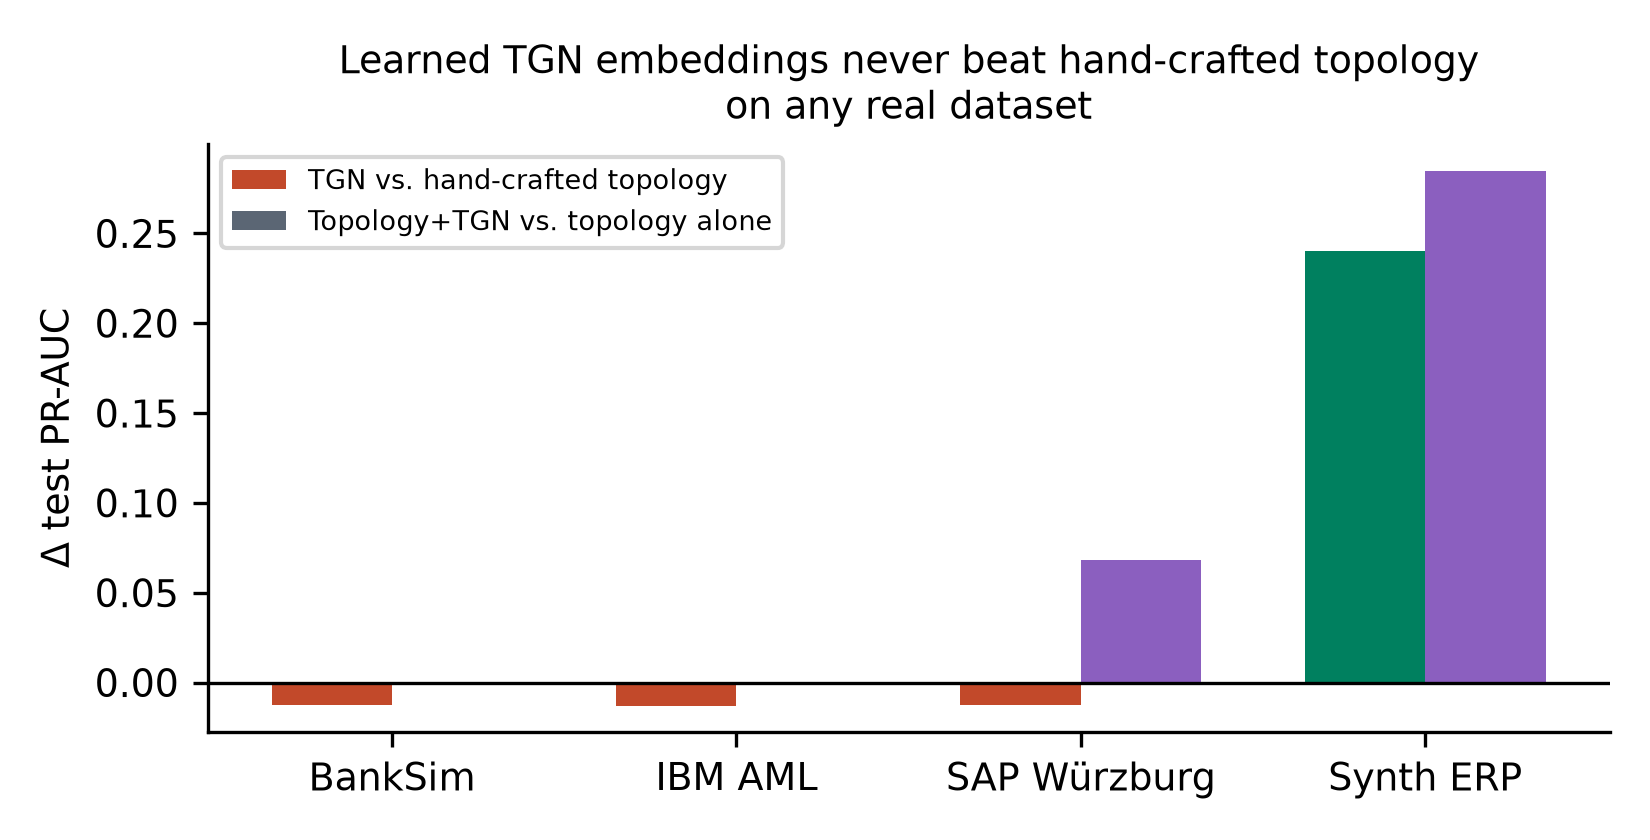
\includegraphics[width=\columnwidth]{figures/modern_tgn_lift_by_dataset.png}
\caption{TGN-vs-topology and combined-vs-topology PR-AUC deltas by dataset (\texttt{modern.json}). The TGN-vs-topology bar is negative on all three real datasets and positive only on the non-evidentiary synth\_erp dataset.}
\label{fig:tgn-lift}
\end{figure}

\subsubsection{Implication for the production system}

Two independent findings close off TGN as a candidate for the served model, both already on the record from this build. First, TGN training is not bit-reproducible across machines even with a fixed seed: re-running the TGN trainer on freshly downloaded copies of the same source data and re-scoring against the committed champion bundle does not reproduce the committed test PR-AUC --- BankSim recomputes to 0.845 against the bundle's recorded 0.938, and SAP Würzburg to 0.098 against the bundle's 0.140 (Section~\ref{sec:threats}, Threats to Validity). Small floating-point differences in CPU-side PyTorch training compound across epochs and propagate through a feature block that carries 17--42\% of the champion model's total SHAP importance (Table~\ref{tab:tgn-lift}), so an offline champion bundle trained on one machine cannot be assumed to reproduce its recorded score on another. Second, and independently disqualifying, the TGN's per-account GRU memory tensor --- the running state that makes its embeddings meaningful at any given point in time --- is never persisted by the training code; it exists only inside the training process and is discarded on exit, so there is no artifact from which a live scoring service could resume the memory a freshly arriving transaction would need.

For these reasons, the production system described in Section~\ref{sec:production} does not serve the TGN-augmented champion at all. It serves a separate, explicitly named \emph{online} bundle --- ordinary features plus hand-crafted topology only, arm B's feature set --- built and reported independently in \texttt{paper/data/online\_bundles.json}: 34 features and test PR-AUC 0.9311 $\pm$ 0.0005 on BankSim, 33 features and 0.1094 $\pm$ 0.0198 on SAP Würzburg, and 28 features and 0.5702 $\pm$ 0.0174 on synth\_erp. IBM AML's online-bundle entry, labeled \texttt{ibm\_aml\_kaggle} (26 features, test PR-AUC 0.5120 $\pm$ 0.0674), is a fresh Kaggle re-download reproduction check, not the same simulator instance behind this section's headline IBM AML numbers, and its PR-AUC is correspondingly far below this section's saturated 1.0000 --- a difference of instance, not of method, and one more reason the two IBM AML number sets in this paper must never be merged. In short: every PR-AUC reported in this section for the ``champion'' or ``combined'' arm describes an offline, research-only model; the number that describes what a live transaction would actually be scored against is the online-bundle figure above, and it excludes TGN entirely.

\subsection{Synthetic Economy: Realism and Augmentation Results}
\label{sec:synthetic-realism}

For every statistic we report on \texttt{synth\_erp}, we ask one question:
does it fall inside the range spanned by the four real datasets
(\texttt{ibm\_aml}, \texttt{banksim}, \texttt{sap\_wurzburg}, \texttt{paysim}),
measured with identical methodology, or outside it? Table~\ref{tab:synth-realism}
answers this for six statistics drawn from \texttt{calibration\_reference.json}
and \texttt{synth\_erp\_realism.json}. The fraud rate, the repeat-pair share
of transactions, and the sender/receiver namespace overlap all land inside
the real span. Three do not, and we report them plainly rather than tuning
them away. Log-amount dispersion (\texttt{log1p\_std} = 2.3256) sits above
every real dataset (span 0.9551--2.0193): the simulated economy mixes
cents-scale retail tickets with treasury sweeps of hundreds of thousands of
dollars in one distribution, a wider mixture than any single-domain real
dataset exhibits — genuine \emph{over}-dispersion, not a defensible match.
Benford mean-absolute-deviation (\texttt{benford\_mad} = 0.0047) is
\emph{lower} than every real dataset (span 0.0142--0.0758): \texttt{synth\_erp}'s
amounts obey Benford's law more cleanly than any real ledger we measured,
itself a realism failure in the opposite direction — real accounting data
carries idiosyncratic roundness and human-entered biases that a mixture of
lognormal generators does not reproduce. Pair reciprocity
(\texttt{pair\_reciprocity} = 0.1356) is roughly $3.0\times$ the real maximum
(0.0446, \texttt{ibm\_aml}): salary-to-purchase circulation and refund/cover
behavior generate more back-and-forth pairs than any of the four real
economies structurally permit. None of these three deviations is hidden in
downstream use: they are why \texttt{synth\_erp} is never treated as evidence
for this paper's central topology claim, only as training material and a
stress test, per the usage policy at the top of this section.

%% FIGURE TODO: grouped bar chart with one bar-triplet per calibration metric
%% (fraud rate, log1p_std, benford_mad, pair_reciprocity, repeat_pair_frac,
%% namespace_overlap): synth_erp value vs. the real-dataset min-max band
%% (shown as a shaded range or error bar), so in-range vs. out-of-range
%% metrics are visually obvious at a glance. Omitted from the body to save
%% space given Table~\ref{tab:synth-realism} already reports the same numbers.

\begin{table}[t]
\centering
\small
\caption{Realism audit: \texttt{synth\_erp} vs.\ the real-dataset reference band (min--max across \texttt{ibm\_aml}, \texttt{banksim}, \texttt{sap\_wurzburg}, \texttt{paysim}). Source: \texttt{calibration\_reference.json}, \texttt{synth\_erp\_realism.json}.}
\label{tab:synth-realism}
\resizebox{\columnwidth}{!}{%
\begin{tabular}{@{}lrrrl@{}}
\toprule
Metric & \texttt{synth\_erp} & Real min & Real max & In band? \\
\midrule
Fraud rate               & 0.4884\% & 0.1236\% & 1.2108\% & Yes \\
Repeat-pair txn.\ share  & 0.8586   & 0.0      & 0.9936   & Yes \\
Namespace overlap        & 0.9410   & 0.0      & 0.9927   & Yes \\
log1p(amount) std.\      & 2.3256   & 0.9551   & 2.0193   & \textbf{No (above)} \\
Benford MAD              & 0.0047   & 0.0142   & 0.0758   & \textbf{No (below)} \\
Pair reciprocity         & 0.1356   & 0.0      & 0.0446   & \textbf{No (3.0$\times$ above)} \\
\bottomrule
\end{tabular}%
}
\end{table}

A more direct realism concern is whether fraud amounts alone give fraud away —
the specific artifact this project identified in \texttt{ibm\_aml} elsewhere in
this paper (fraud amounts distinctively \emph{small}, amount-ratio 0.068,
globally separable at ROC-AUC $\approx 0.91$). On \texttt{synth\_erp}, the
median fraud amount (\$1{,}692.59) is 23.79$\times$ the median benign amount
(\$71.14; the equivalent ratio in \texttt{banksim}, from
\texttt{calibration\_reference.json}, is 11.9$\times$), and a univariate
log-amount classifier reaches ROC-AUC 0.8078 overall (KS statistic 0.604
between the fraud and benign log-amount distributions) — at first glance a
fraud population skewed to B2B-sized amounts in a retail-heavy economy.
Restricted to the amount band where 93\% of fraud actually lives
(\$300--\$20{,}000, $n=5{,}228$ fraud rows in band), that same classifier
collapses to ROC-AUC 0.4911 — indistinguishable from chance. Fraud amounts
are globally distinguishable only because fraud skews toward a coarser amount
regime than the bulk of retail traffic; \emph{within} its own regime, amount
carries essentially no signal, forcing any detector toward behavioral or
structural evidence rather than a one-column amount rule — the opposite of
the \texttt{ibm\_aml} artifact, and a deliberate design target corroborated
here after the fact rather than asserted in advance.

\subsubsection{Adversarial Tabular-Leak Probe}
\label{sec:synthetic-leakprobe}

A realistic amount distribution does not rule out a cheap categorical
shortcut elsewhere in the table — the same class of hidden bias that motivates
auditing tabular fraud-evaluation datasets for shortcut features before
trusting them~\cite{jesus2022turning}. We therefore ran an automated probe over 16
candidate rules — every \texttt{tx\_type} indicator, an account-creation-date
indicator on each side of the transaction, and pairwise conjunctions of the
two — scoring each rule's support, precision, recall of fraud, and lift over
the 0.4884\% base rate. Table~\ref{tab:synth-leakprobe} reports the eight
highest-lift rules out of the 16 tested. Three flow types
(\texttt{tx\_type=payroll}, \texttt{tx\_type=recurring\_bill},
\texttt{tx\_type=refund}) and their conjunctions with a mid-year account
carry \emph{zero} fraud whatsoever (lift 0.0) — no scenario in the generator
routes any of the five typologies onto these three rails at all, which is a
genuine (if narrow) gap in coverage rather than a realism strength.

The rule the probe itself records as worst,
\texttt{tx\_type=transfer \& dest\_created\_midyear}, reaches a lift of
$19.0\times$ the base rate, support of 26{,}420 transactions, precision of
9.29\%, and recovers 43.75\% of all fraud in a single two-clause rule. The
dataset's own automated gate does not classify this as a leak
(\texttt{leak\_flag} = \texttt{false}, its precision bar sitting well above
what this rule reaches), and a rule flagging under 10\% of the transactions it
fires on as fraud is far from the near-deterministic, one-line shortcuts the
generator's earlier drafts contained before an adversarial review removed
them. Still, a rule with 19$\times$ lift and 44\% recall is a real,
exploitable regularity, not a non-finding, and we report it rather than let a
binary pass/fail flag stand in for a reader's own judgment of where
``legitimate risk factor'' ends and ``tabular leak'' begins. A transaction
moving through the \texttt{transfer} rail toward an account opened within the
same year is a defensible real-world risk heuristic — mid-year account
creation correlates with fraud in practice, not only in this simulation — but
we flag it here precisely so that any model trained on \texttt{synth\_erp}
can be checked for whether it quietly learned this shortcut instead of the
intended structural and behavioral signal.

\begin{table}[t]
\centering
\scriptsize
\caption{Adversarial tabular-leak probe, top 8 of 16 rules by lift. Base fraud rate 0.4884\%. Source: \texttt{synth\_erp\_realism.json}, \texttt{tabular\_leak\_probe}.}
\label{tab:synth-leakprobe}
\resizebox{\columnwidth}{!}{%
\begin{tabular}{@{}lrrrr@{}}
\toprule
Rule & Support & Precision & Recall & Lift \\
\midrule
\texttt{transfer \& dest\_midyear}$^\dagger$ & 26{,}420 & 0.0929 & 0.4375 & \textbf{19.0} \\
\texttt{dest\_created\_midyear}         & 67{,}621  & 0.0502 & 0.6049 & 10.3 \\
\texttt{tx\_type=transfer}              & 94{,}781  & 0.0385 & 0.6500 & 7.9 \\
\texttt{vendor\_payment \& dest\_midyear}$^\dagger$ & 25{,}781 & 0.0316 & 0.1451 & 6.5 \\
\texttt{sale \& dest\_midyear}$^\dagger$          & 8{,}131   & 0.0146 & 0.0212 & 3.0 \\
\texttt{src\_created\_midyear}          & 156{,}550 & 0.0113 & 0.3147 & 2.3 \\
\texttt{reimbursement \& dest\_midyear}$^\dagger$ & 741       & 0.0081 & 0.0011 & 1.7 \\
\texttt{tx\_type=reimbursement}         & 12{,}236  & 0.0079 & 0.0173 & 1.6 \\
\bottomrule
\end{tabular}%
}
\vspace{2pt}
\raggedright\scriptsize $^\dagger$\texttt{dest\_midyear} abbreviates \texttt{dest\_created\_midyear}.
\end{table}

\subsubsection{The Augmentation Transfer Probe}
\label{sec:synthetic-augmentation}

The realism and leak audits above establish what \texttt{synth\_erp} is
calibrated well enough to be used \emph{for}. The most direct test of the
narrower, practical question — does adding \texttt{synth\_erp} rows to a real
dataset's training split make its fraud model better? — is a paired
augmentation experiment: for each of three real datasets, train an XGBoost
model~\cite{chen2016xgboost} three ways (real data only; real data with all
1{,}148{,}503 \texttt{synth\_erp} rows pooled into the training split; and
\texttt{synth\_erp} data only, evaluated zero-shot on the real test split),
each averaged over three seeds, under the same time-aware split, class-weight
imbalance handling, and validation-tuned threshold used throughout this paper.
Table~\ref{tab:synth-augmentation} reports the result, and it is unambiguous:
pooling synthetic rows into training \emph{hurts} test PR-AUC on every one of
the three real datasets tested. \texttt{banksim} falls from
$0.8669\pm0.0031$ (real-only) to $0.7610\pm0.0022$ (real+synth), a paired
per-seed delta of $-0.1059\pm0.0011$; \texttt{ibm\_aml} falls from an
already-saturated $0.99999\pm0.00001$ to $0.9954\pm0.0013$,
$\Delta=-0.0046\pm0.0013$ — small in absolute terms, but the baseline leaves
almost no headroom to fall into, so even this small drop is a consistent,
same-direction result; and \texttt{sap\_wurzburg} — on only 25 test-set
frauds, the same small-sample caveat that applies to every
\texttt{sap\_wurzburg} result in this paper — falls from $0.1366\pm0.0446$ to
$0.0293\pm0.0033$, $\Delta=-0.1073\pm0.0417$.
The mechanism is unsurprising in hindsight given Sec.~\ref{sec:synthetic-realism}:
a single tree ensemble fit jointly over two economies with measurably
different amount dispersion and reciprocity structure pulls its splits toward
the pooled distribution, at the real dataset's expense. We report this as a
clean negative result rather than qualify it away: \emph{naive} pooled
augmentation with this dataset, under this protocol, does not help, on any
real dataset we tested it against.

\begin{table}[t]
\centering
\small
\caption{Augmentation transfer probe: XGBoost PR-AUC, 3-seed mean $\pm$ std. \texttt{synth\_only} is zero-shot (trained solely on \texttt{synth\_erp}, evaluated on the real test split). Source: \texttt{augmentation.json}.}
\label{tab:synth-augmentation}
\resizebox{\columnwidth}{!}{%
\begin{tabular}{@{}lrrrr@{}}
\toprule
Dataset & Real-only & Real+synth & $\Delta$ & Synth-only \\
\midrule
\texttt{banksim} ($n{=}1320$)      & 0.8669$\pm$0.0031 & 0.7610$\pm$0.0022 & $-$0.1059$\pm$0.0011 & \textbf{0.7243$\pm$0.0079} \\
\texttt{ibm\_aml} ($n{=}377$)      & 0.99999$\pm$0.00001 & 0.9954$\pm$0.0013 & $-$0.0046$\pm$0.0013 & 0.0017$\pm$0.0006 \\
\texttt{sap\_wurzburg} ($n{=}25$)  & 0.1366$\pm$0.0446 & 0.0293$\pm$0.0033 & $-$0.1073$\pm$0.0417 & 0.0008$\pm$0.0001 \\
\bottomrule
\end{tabular}%
}
\end{table}

There is exactly one genuinely positive number in this experiment, and it is
a narrower, different claim than ``synthetic data helps supervised
training'': the \texttt{synth\_only} zero-shot column for \texttt{banksim}.
A model that has \emph{never seen a single real BankSim row} — trained
entirely on \texttt{synth\_erp}, evaluated as-is on real, held-out
\texttt{banksim} test data — scores $0.7243\pm0.0079$ PR-AUC, recovering
83.6\% of the $0.8669$ real-trained baseline, at precision@100 of
$0.99\pm0.0082$ against the real-trained baseline's perfect $1.00$; chance at
this split's 1.21\% fraud rate is on the order of $0.01$--$0.02$ PR-AUC, so
this is far from a vacuous transfer. The same zero-shot comparison fails on
\texttt{ibm\_aml} ($0.0017$ PR-AUC against a $0.99999$ real-trained ceiling —
unsurprising, since \texttt{ibm\_aml}'s giveaway-small fraud amounts are
inverted relative to \texttt{synth\_erp}'s B2B-skewed fraud) and on
\texttt{sap\_wurzburg} ($0.0008$ PR-AUC, 25 test frauds, too small to support
any transfer claim). We read the \texttt{banksim} result as evidence that the
synthetic economy teaches \emph{transferable structural and behavioral
discrimination} that generalizes to a real domain it structurally resembles —
not as evidence that pooling synthetic rows into a real training set is a
useful augmentation recipe. These are two different claims, only one of which
this experiment supports; we are careful not to let the positive framing of
the zero-shot result launder the negative framing of the pooled-augmentation
result three rows above it.

\subsubsection{Summary and Scope}

\texttt{synth\_erp} is a large, ERP-flavored, multi-typology synthetic ledger
built under a binding non-circularity constraint and audited, after the fact,
against four real datasets on realism, tabular leakage, and downstream
transfer. It matches the real fraud-rate, repeat-pair, and namespace-overlap
bands; it is measurably over-dispersed in amount and reciprocity and
unrealistically Benford-clean relative to every real dataset compared against
it; its cheapest categorical shortcut reaches 19$\times$ lift and 44\% recall
without being flagged as a formal leak, a judgment call we surface rather
than hide; and pooling it into real training data hurts every real dataset's
PR-AUC we tested, its one positive contribution being a narrower zero-shot
transfer result on the one real dataset it structurally resembles.
Consistent with the usage policy stated at the outset, none of this
section's numbers are used anywhere in this paper as evidence for the
central topology claim (Sec.~\ref{sec:ablation}); \texttt{synth\_erp}'s role
is training material, a per-typology stress test, and demo content for the
audit console (Sec.~\ref{sec:system}), never proof.

\subsection{Explainable Audit Alerts: Results}\label{sec:explain-results}
Three of the four datasets reach perfect precision at their operating $k$
(Table~\ref{tab:alert_precision}): every one of BankSim's top 15, IBM AML's
top 20, and synth\_erp's top 20 test-period alerts is a labelled fraud. IBM
AML's 1.00 should not be over-read, however: its baseline model is already
saturated at $\mathrm{PR\text{-}AUC}\approx0.99$ (the ablation study reported earlier in this paper),
so a perfect top-$k$ here is consistent with the amount signal alone doing
the work and does not, on its own, demonstrate that topology mattered for
these particular alerts -- three of the twenty carry no reconstructable
fan-in or cycle evidence at all (\texttt{evidence\_type\_counts.none}=3),
meaning their risk drivers were purely \texttt{ordinary}/\texttt{tgn}.

SAP Würzburg is the outlier the ablation predicts: precision@10 is 0.20 (2 of
10), the weakest by a wide margin, the direct operational consequence of the
dataset's negative marginal structural lift reported elsewhere in this
paper, compounded by only 25 labelled test frauds. Every one of its ten
alerts is nonetheless a syntactically well-formed, replay-verified fan-in --
destinations collecting from 166 to 271 distinct senders in-window --
because those accounts are simply high-traffic general-ledger hubs
(\texttt{GL:895000}, \texttt{GL:300000}), not because fraud is present. This
is the clearest illustration in the paper of what Layer 2 actually
guarantees: the evidence is provably consistent with what the model saw,
never a guarantee that what the model saw was fraud. (Its test-partition
size also differs by source file: \texttt{final\_champions.json}, which
produced this bundle, reports 40{,}116 test rows / 25 frauds, while
\texttt{ablation.json}'s separately-run partition-aware split reports
40{,}139 -- the two pipeline runs are not the same split and should not be
merged.)

\subsubsection{Global Attribution Is Dataset-Specific, Not Universal}
Averaging $|\text{SHAP}|$ over a sample of each dataset's test rows
(\texttt{final\_champions.json}: \texttt{shap\_global\_top20}, 50{,}000
sampled rows for BankSim/IBM~AML/synth\_erp and the full 40{,}114-row test
partition for SAP Würzburg, since \texttt{bundle\_metadata.json} does not
itself carry per-feature magnitudes) shows that no single family dominates
across datasets (Table~\ref{tab:global_shap}).

\begin{table}[t]
\centering
\caption{Top-3 globally attributed features per dataset by mean $|$SHAP$|$ (margin space), with family tag (\texttt{paper/data/final\_champions.json}).}
\label{tab:global_shap}
\small
\begin{tabular}{lclr}
\toprule
Dataset & Rank & Feature (family) & Mean $|$SHAP$|$ \\
\midrule
\multirow{3}{*}{BankSim}
 & 1 & \texttt{category\_es\_transportation} (ordinary) & 0.675 \\
 & 2 & \texttt{fan\_in} (topology) & 0.609 \\
 & 3 & \texttt{dest\_in\_degree} (topology) & 0.558 \\
\midrule
\multirow{3}{*}{IBM AML}
 & 1 & \texttt{lap\_out\_recur} (topo.-amt-derived) & 0.588 \\
 & 2 & \texttt{log\_amount} (ordinary) & 0.296 \\
 & 3 & \texttt{lap\_out\_payees} (topo.-amt-derived) & 0.079 \\
\midrule
\multirow{3}{*}{SAP Würzburg}
 & 1 & \texttt{fan\_in} (topology) & 0.189 \\
 & 2 & \texttt{dest\_count\_prior} (ordinary) & 0.088 \\
 & 3 & \texttt{log\_amount} (ordinary) & 0.028 \\
\midrule
\multirow{3}{*}{synth\_erp}
 & 1 & \texttt{log\_amount} (ordinary) & 0.718 \\
 & 2 & \texttt{tgn\_edge\_expectedness} (tgn) & 0.407 \\
 & 3 & \texttt{dest\_in\_degree} (topology) & 0.357 \\
\bottomrule
\end{tabular}
\end{table}

BankSim's single most-attributed feature globally is a merchant-category
indicator, not a topology feature -- \texttt{fan\_in} and
\texttt{dest\_in\_degree} rank second and third -- even though BankSim is
the dataset with the strongest validated structural lift in this paper.
Amount and category signal dominates the average attribution even where
topology genuinely helps; the two findings are compatible because global
mean $|\text{SHAP}|$ and marginal ablation lift answer different questions
(which features move scores the most, vs.\ how much test-set PR-AUC a
feature group adds).

IBM AML's global top feature is \texttt{lap\_out\_recur}, tagged
\texttt{topology-amount-derived} rather than pure \texttt{topology} --
confirming at the dataset level the alert-level pattern noted above, and
consistent with \texttt{final\_champions.json}'s own recorded caveat for
this dataset (``baseline is amount-saturated ($\mathrm{PR\text{-}
AUC}\sim1.0$): margins here are uninformative''). No genuine cycle feature
appears in its top 20 at all, despite cycles accounting for 8 of its 20
alert-evidence blocks -- the model leans on the amount-derived lapping
proxy while Layer 2's independent replay still finds and shows a real
closed loop.

SAP Würzburg is the only dataset whose global top feature is a
\emph{pure} topology column (\texttt{fan\_in}), yet it also has the
negative marginal structural lift and the worst alert precision in this
paper: mean $|\text{SHAP}|$ measures how much a feature moves the score on
average, not whether that movement is correct, and \texttt{fan\_in} can be
the model's largest lever while remaining a poor discriminator when the
underlying counts reflect a handful of high-traffic GL hub accounts rather
than fraud. synth\_erp -- sanity/demonstration data, never thesis evidence --
shows a third pattern: \texttt{log\_amount} leads, with a learned TGN
feature and a topology feature close behind, echoing the earlier finding
that on this dataset learned and hand-engineered structure are
complementary rather than either dominating.

Together, Tables~\ref{tab:alert_precision} and~\ref{tab:global_shap} argue
against any single sentence like ``the model relies on graph structure'':
which family dominates, and whether that reliance is well-founded, is
dataset-specific. The console's honesty about that -- visible family tags,
replay-verifiable evidence, and a \texttt{ground\_truth\_label} kept for
research transparency but never surfaced to a real reviewer -- is the point
of the two-layer design, not a substitute for the ablation evidence that
grounds it.

\subsection{The Online/Offline Serving Gap}\label{sec:system-serving}

The champion models evaluated earlier in this paper (Section~V) include a Temporal Graph Network (TGN) embedding stage~\cite{rossi2020temporal} feeding an XGBoost head~\cite{chen2016xgboost}. These champions are \emph{not} servable online, and the paper makes no claim that they are. Two independent problems rule it out. First, TGN inference requires a memory tensor built by replaying a transaction sequence through the trained network; nothing in this build persists that tensor, so scoring a single live transaction would require replaying the dataset's entire prior history on every request — the opposite of the online engine's O(1)-per-feature design. Second, and more fundamentally, TGN training on this codebase is not bit-reproducible across machines even with a fixed seed: re-running \texttt{modeling.tgn} on freshly downloaded, same-source data and re-scoring against the committed champion bundle diverges substantially (documented in \texttt{docs/BUILD\_SPEC.md} as a reproduction failure on both banksim and sap\_wurzburg test folds), because small floating-point differences in CPU training compound over epochs through a component that accounts for 17--42\% of the champion's feature importance. A component that will not reproduce its own training run on the same machine is not a component a production system should be handed authority to persist and reload.

The deployed artifact is therefore a deliberately smaller "online" bundle, trained on ordinary and topology features only, with the TGN family dropped entirely rather than approximated. This is verifiable directly in the two bundle manifests: the online bundle's feature count is, dataset by dataset, exactly the ordinary-plus-topology subtotal of the champion's own feature-family breakdown (banksim: $21+13=34$; sap\_wurzburg: $20+13=33$; synth\_erp: $15+13=28$; against champion totals of 99, 98, and 93 respectively, each with 65 TGN dimensions removed) — confirming the online bundle is the champion's own feature set with TGN excised, not an independently retrained approximation. Table~\ref{tab:online-gap} reports what that exclusion costs in test PR-AUC, computed directly from \texttt{paper/data/final\_champions.json} (champion) and \texttt{paper/data/online\_bundles.json} (online).

\begin{table}[t]
  \centering
  \small
  \caption{Test PR-AUC: offline TGN-inclusive champion vs.\ the deployed online (ordinary+topology only) bundle, same dataset instance, 3 seeds each.}
  \label{tab:online-gap}
  \begin{tabular}{lccc}
    \toprule
    Dataset & Champion & Online & Gap \\
    \midrule
    banksim      & $0.93637 \pm 0.00154$ & $0.93114 \pm 0.00045$ & $0.00523$ \\
    sap\_wurzburg & $0.1557 \pm 0.07166$  & $0.10939 \pm 0.01982$ & $0.04631$ \\
    synth\_erp    & $0.77845 \pm 0.00526$ & $0.57018 \pm 0.01744$ & $0.20827$ \\
    \bottomrule
  \end{tabular}
\end{table}

The cost of going online is small on banksim (0.005 PR-AUC) but is not uniformly small: synth\_erp pays roughly 0.21 PR-AUC and sap\_wurzburg roughly 0.05, consistent with a component contributing 17--42\% of feature importance being removed entirely. sap\_wurzburg's champion figure also carries the small-test-fold caveat attached to that dataset elsewhere in this paper — both its ablation split and its champion split contain only 25 fraud cases in the test fold, so both the champion and online numbers for that dataset should be read as high-variance point estimates, not precise costs. IBM AML is deliberately omitted from Table~\ref{tab:online-gap}: the champion figure in \texttt{final\_champions.json} (\texttt{ibm\_aml}, PR-AUC $1.0\pm0.0$, consistent with the baseline-saturation finding reported elsewhere in this paper) is trained on a different underlying data acquisition than \texttt{ibm\_aml\_kaggle} (PR-AUC $0.512\pm0.06743$), the fresh Kaggle re-download the online bundle is actually trained and served on. Reporting a "gap" between two different simulator instances would misstate the cost of removing TGN as the cost of a different dataset entirely, so no such number is reported; \texttt{ibm\_aml\_kaggle}'s figure stands on its own as the deployed bundle's performance on the data it was actually built from.

A second, smaller and more deliberate divergence exists between the two paths' ordinary-feature computation. The batch engine's expanding per-account z-score uses the textbook two-pass variance formula ($\overline{x^2} - \bar{x}^2$), which suffers catastrophic cancellation for accounts whose historical amounts are nearly identical — verified on the full banksim dataset to produce spurious $|z|>1000$ values (observed up to $\sim\!10^8$) on 1{,}238 of 594{,}643 rows (0.21\%), where a numerically stable computation should return a near-zero or undefined value. \texttt{app/services/online\_ordinary.py} computes the same statistic via Welford's algorithm, which does not exhibit this failure mode and instead returns \texttt{NaN}. Rather than reproduce a known instability from the locked research pipeline into new serving code for the sake of train/serve identity, the online path uses the numerically correct formulation and accepts a small, disclosed, and precisely quantified skew on 0.21\% of rows as the honest cost of not shipping a bug on purpose.


\subsection{Measured Performance, Concurrency, and Recovery}\label{sec:system-performance}

Query optimization was driven by captured \texttt{EXPLAIN (ANALYZE, BUFFERS)} plans against a reproducibly bulk-seeded dev database (5{,}000 vendors, 40{,}000 invoices, 23{,}929 payments, 5{,}000 audit alerts; seed 42; \texttt{ANALYZE} re-run after load so planner statistics are current), not guessed indexes. Table~\ref{tab:queries} reports the result honestly, including the one index that did not help: a composite index added to the vendor-scoped invoice listing on the expectation that it would repeat the first query's win did not change the query plan at all, because at this dataset's distribution (roughly 8 invoices per vendor) sorting that few rows is already cheaper than the planner switching indexes. It remains in the schema — cheap to maintain, and the correct choice the moment a single vendor's invoice volume becomes skewed — but is reported as a non-win rather than silently dropped or claimed as a success it was not.

\begin{table}[t]
  \centering
  \scriptsize
  \resizebox{\columnwidth}{!}{%
  \begin{tabular}{lp{4.3cm}p{4.1cm}c}
    \toprule
    Query & Before & After & Speedup \\
    \midrule
    Paid invoices, newest-first (\texttt{status='paid'} \texttt{ORDER BY invoice\_date DESC LIMIT 50}) &
      Bitmap Heap Scan $\to$ top-$N$ heapsort; 875 buffer hits; 6.331~ms &
      Index Scan Backward, no sort; 50 buffer hits; 0.301~ms & $\sim\!21\times$ \\
    \addlinespace
    Alert queue (\texttt{ORDER BY score DESC LIMIT 50}) &
      No index existed; seq-scan-and-sort baseline never captured at scale\textsuperscript{a} &
      Index Scan (DESC); 0.236~ms & --- \\
    \addlinespace
    Vendor-scoped invoices (\texttt{vendor\_id=?} \texttt{ORDER BY id LIMIT 50}) &
      Bitmap Index Scan on \texttt{vendor\_id} + small sort; 0.253~ms &
      \emph{Same plan} -- new composite index not selected; 0.317~ms & none \\
    \bottomrule
  \end{tabular}}
  \caption{Module 7 query optimization, before/after \texttt{EXPLAIN (ANALYZE, BUFFERS)} on a bulk-seeded dev database. Row 3 is reported as a genuine non-win, not silently dropped.}
  \label{tab:queries}
\end{table}
\vspace{-0.6em}
{\scriptsize\textsuperscript{a}The \texttt{audit\_alerts} table was empty during earlier module testing; no pre-index baseline exists at production row counts, so degradation was inferred, not measured.\par}

Redis-backed response caching (route+params+tenant+role key, ETag/304 support, explicit invalidation on write) and all four new indexes ship as ordinary \texttt{CREATE INDEX} migrations rather than \texttt{CONCURRENTLY} builds — an acceptable simplification against an empty or lightly loaded dev-scale table, but a production rollout against a live, concurrently written table should use \texttt{postgresql\_concurrently=True} outside a transaction block to avoid holding write locks for the duration of the index build.

Observability runs as a verified Prometheus/Grafana/Uptime Kuma stack, not a planned one. Prometheus scrapes \texttt{/metrics} every 10~seconds with the \texttt{shadow-ledger-api} target confirmed healthy; a Grafana dashboard ("Shadow Ledger — Overview") is auto-provisioned alongside the datasource and exposes request rate and 5xx rate by route, p95 latency by route, fraud-scoring latency p50/p95/p99, cache hit rate, and duplicate-payment attempts. \texttt{fraud\_scoring\_latency\_seconds\{dataset\}} is the histogram the paper's sub-200~ms p95 latency target is measured against, reflecting the online path's O(1)-per-feature design (Section~\ref{sec:system-serving}): topology lookup, Welford-based ordinary features, one small XGBoost \texttt{DMatrix} predict, and TreeSHAP, with no whole-stream replay on the request path. Uptime Kuma probes \texttt{/health} and \texttt{/ready} every 30~seconds; \texttt{/ready} already returns 503 the instant the database, Redis, or the scoring registry is unavailable, so the monitor's job is only to alert on a non-200, not to implement the health logic itself. Error logging is structured JSON with correlation-id propagation from the access log through every service call (\texttt{app/core/logging.py}), live since the project's first module and the actual mechanism every bug found during query optimization and testing was diagnosed from; a self-hosted GlitchTip instance was scoped but not deployed, since it requires its own Postgres database, Redis, and Celery worker rather than a docker-compose add-on line — \texttt{GLITCHTIP\_DSN} is already read by \texttt{app/core/config.py} as a drop-in point once a target instance exists.

Concurrency, load, and recovery were exercised as k6 scripts and a scripted backup/restore drill, with every figure below taken from an actual run (\texttt{docs/TESTING\_MODULE9.md}), not a projection. The duplicate-payment race (\texttt{tests/load/payment\_race.js}) is the automated form of the defense in Section~\ref{sec:system-integrity}: 30 virtual users fire truly concurrent payment requests at one invoice, each with a distinct idempotency key, so that the only thing standing between them and a double payment is the row lock and unique index, not idempotency replay. The mixed-workload ramp (\texttt{tests/load/mixed\_workload.js}) drives a 70\%~browse / 20\%~invoice-submission / 10\%~alert-queue-read mix from 0 to 500 concurrent users against a single dev-mode \texttt{uvicorn} process with no worker pool and a 40-connection database pool, deliberately reported as a degradation-point measurement rather than a pass/fail gate.

\begin{table}[t]
  \centering
  \scriptsize
  \caption{Module 9 concurrency and recovery drills — measured results.}
  \label{tab:reliability}
  \begin{tabular}{p{0.22\columnwidth}p{0.36\columnwidth}p{0.32\columnwidth}}
    \toprule
    Drill & Configuration & Result \\
    \midrule
    Duplicate-payment race & k6, 30 VUs, 1 invoice, distinct idempotency keys & 1/30 succeeded, 29/29 rejected (\texttt{duplicate\_payment}); DB confirms exactly 1 payment row; successful-request latency avg 267\,ms, p95 807\,ms \\
    \addlinespace
    Mixed workload ramp & k6, 0$\to$50$\to$200$\to$500 VUs, single uvicorn worker, 40-conn.\ DB pool & 39{,}727 requests attempted, 28{,}642 completed; overall p95 8.18\,s; error rate 4.42\% ($<$5\% threshold passed; $p95<1$\,s threshold \textbf{failed}) \\
    \addlinespace
    Backup/restore drill & \texttt{pg\_dump -Fc} $\to$ clean throwaway DB; row-count + payment-total fingerprint compare & Quiescent run: match=true, RTO$=3.07$\,s (dump 0.95\,s/6.99\,MB, restore 2.12\,s); a run taken concurrently with active writes legitimately reports match=false (Postgres MVCC), reproduced again in the most recent committed drill \\
    \bottomrule
  \end{tabular}
\end{table}

The mixed-workload result is reported as found: the system clearly degrades before reaching 500 concurrent users, with I/O timeouts appearing during the highest-VU stage and overall p95 latency an order of magnitude above the 1-second threshold. This is expected of a single dev-mode process and is the useful output of the test — it names horizontal scaling (\texttt{--workers~N}, a larger pool, or multiple instances behind a load balancer) as the concrete next step for a production rollout, rather than asserting a latency number the current deployment configuration cannot support. The backup/restore drill's own history is a second methodology finding worth stating rather than hiding: an initial drill run taken while the mixed-workload test was still writing to the database correctly reported a fingerprint mismatch, not because backup or restore is broken, but because \texttt{pg\_dump} does not block concurrent writers under Postgres MVCC, so a fingerprint query issued moments before the dump can legitimately diverge from what the dump itself captures. The most recently committed drill artifact (\texttt{infra/backups/last\_drill\_report.json}) reproduces exactly this pattern (match=false, RTO 2.85\,s) against live traffic, while the clean, quiescent-database run reported in Table~\ref{tab:reliability} passed. The operational implication is direct: a production backup schedule needs either a quiescent window, a shared \texttt{pg\_export\_snapshot()}, or reliance on the continuous WAL archiving already enabled (\texttt{archive\_mode=on}) for point-in-time recovery — none of which this session exercised end-to-end, and all of which are named as the concrete next drill rather than assumed solved.


\subsection{Discussion: Threats to Validity and Limitations}\label{sec:limitations}\label{sec:threats}

The preceding sections report several results this paper is obligated, by its
own stated methodology, never to soften: a negative topology lift on SAP
W\"urzburg, an uninformative comparison on a saturated IBM AML baseline, a
single-seed ablation, and a deployed model that is provably not the model
evaluated as the research champion. This section collects those admissions in
one place, cross-referenced rather than re-derived, and adds several threats
not yet raised elsewhere in the paper: the measured cost of naive synthetic
augmentation, a numerical-stability defect that quietly touches every headline
number in this study rather than only the serving path, and the scope
boundaries of the production system's access-control and deployment model.
Table~\ref{tab:threats-summary} summarizes all seven; the remainder of this
section explains each.

\begin{table}[t]
\centering
\caption{Threats to validity, at a glance. Every magnitude is read directly from a named artifact file, never re-derived here.}
\label{tab:threats-summary}
\resizebox{\columnwidth}{!}{%
\scriptsize
\begin{tabular}{p{2.6cm}p{4.0cm}p{2.6cm}}
\toprule
Threat & Magnitude / evidence & Disclosure \\
\midrule
Single-seed ablation, no CIs & IBM AML full-model lift $+0.00792$ is below the project's own $\sim$0.01 noise floor & \S\ref{sec:ablation-stats}; 3-seed champion partially corroborates \\
\addlinespace
TGN not bit-reproducible & BankSim $0.938\to0.845$; SAP W. $0.140\to0.098$, fixed seed, same source data, different machine & \texttt{docs/BUILD\_SPEC.md}; \S\ref{sec:system-serving} \\
\addlinespace
Batch z-score instability & 1{,}238/594{,}643 (0.21\%) BankSim rows, $|z|>10^3$--$10^8$ from catastrophic cancellation & Online engine uses Welford; batch pipeline uncorrected \\
\addlinespace
Synthetic augmentation hurts & $\Delta$PR-AUC $-0.1059$/$-0.00455$/$-0.10725$ on 3 real datasets, all 3 seeds each & Never used in the deployed bundle's training data \\
\addlinespace
SAP W. small test fold & 25 test frauds; 3-seed champion std $\pm0.0717$ on mean $0.1557$ (46\% rel.) & Flagged high-variance at every occurrence \\
\addlinespace
Deployed $\neq$ champion & Online-bundle gap $0.005$--$0.208$ PR-AUC by dataset & Table~\ref{tab:online-gap}; every PR-AUC labeled champion/online \\
\addlinespace
Coarse RBAC, single tenant & 3 roles, no maker--checker chain; no cross-org isolation tested & Named explicitly as unevaluated scope \\
\bottomrule
\end{tabular}}
\end{table}

\subsubsection{Statistical power: one seed is not an estimate}\label{sec:limitations-stats}
The seven-arm ablation that produces this paper's headline lift numbers
(Table~\ref{tab:ablation-lifts}) is a single training run per arm, seed 42,
with no repeated trials, no confidence intervals, and no significance test of
any kind. \S\ref{sec:ablation-stats} already applies the project's own
$\sim$0.01 PR-AUC noise-floor heuristic to this fact and concludes that IBM
AML's full-model structure lift ($+0.00792$) cannot be distinguished from zero
on the evidence available; we restate it here as what it is: not a p-value,
but an informal threshold the project's own harness code uses to decide when
a difference is worth interpreting at all. No formal bootstrap or paired test
has been run anywhere in this study to replace that heuristic. The separate
three-seed champion runs in \texttt{final\_champions.json} corroborate the
qualitative picture -- BankSim stable at $0.9364\pm0.0015$, SAP W\"urzburg
volatile at $0.1557\pm0.0717$ -- but they evaluate a different, TGN-inclusive
feature set on a (mostly) different split convention, so they are
corroboration, not a repetition of the ablation itself. SAP W\"urzburg's 25
test-split frauds are, on their own, close to a hard ceiling on what any
single-dataset PR-AUC estimate on this data can support; we treat its
negative lift as directionally credible but numerically imprecise throughout,
never as a precise point estimate. Even the split denominators behind this
result are not perfectly reconciled: \texttt{ablation.json} and
\texttt{final\_champions.json} report two slightly different partition-aware
split sizes for SAP W\"urzburg ($120{,}411$/$40{,}137$/$40{,}139$ vs.\
$120{,}341$/$40{,}114$/$40{,}116$, a $0.06\%$ difference, \S\ref{sec:protocol}),
traced to separate ETL passes but not further diagnosed.

\subsubsection{Two disclosed non-reproducibilities}
Two independent findings surfaced during this build's own reproduction
attempts, both load-bearing enough to affect how every TGN-inclusive number
in this paper should be read. First, re-training the TGN encoder on freshly
downloaded copies of the same source data, with the same fixed seed, does
not recover the committed champion bundle's test PR-AUC: BankSim recomputes
to $0.845$ against the bundle's recorded $0.938$, and SAP W\"urzburg to
$0.098$ against $0.140$ (\texttt{docs/BUILD\_SPEC.md}; \S\ref{sec:system-serving}).
CPU-side floating-point differences in PyTorch training compound across
epochs and propagate through a feature block carrying 1.9--42.0\% of the
champion model's SHAP importance depending on dataset. Practically, the
champion PR-AUC figures reported in this paper are this machine's own
measurement, not a constant guaranteed to reproduce on different hardware
with the same seed and code -- a property one would not expect to have to
state for a gradient-boosted tree, but must, because the TGN stage feeding
it is not deterministic across machines.

Second, and unrelated to cross-machine reproducibility, the batch feature
pipeline's expanding per-account z-score uses the textbook two-pass variance
formula ($\overline{x^2} - \bar{x}^2$), subject to catastrophic cancellation
for accounts whose historical amounts are nearly identical. Quantified on the
full BankSim dataset, this produces spurious $|z|>1{,}000$ values (observed
up to $\sim\!10^8$) on $1{,}238$ of $594{,}643$ rows ($0.21\%$), where a
stable computation returns a near-zero or undefined value. This is not
merely a serving-time footnote: the identical formula runs across all four
datasets' batch builds, so every headline ablation and champion PR-AUC in
this paper -- not only the BankSim figure it is quantified on -- was computed
with this instability present somewhere upstream, at an unmeasured rate on
the other three datasets. The online engine
(\texttt{app/services/online\_ordinary.py}) uses Welford's algorithm
instead, which does not fail this way; this was a deliberate choice to ship
correct code going forward rather than replicate a known bug for train/serve
identity, and it is the one place the offline and online paths diverge by
construction rather than by TGN's absence alone. The batch pipeline itself
remains uncorrected -- fixing it would move this paper's own headline numbers
after the fact -- so we disclose the defect precisely rather than patch it
mid-study.

\subsubsection{Synthetic data: barred as evidence, and measurably harmful as augmentation}
synth\_erp is this project's own generated corpus, and the project's binding
policy treats it as a stress-testing environment only, never as thesis
evidence -- precisely to avoid grading its own homework with data built to
contain the structure the paper argues for. Its largest-in-study topology
lift ($+0.4031$ PR-AUC, $246.8\%$ relative) is reported in \S\ref{sec:ablation}
under that explicit caveat and is not treated as support for this paper's
central claim.

A second, distinct question -- does adding synth\_erp rows to a \emph{real}
dataset's training set help a real model -- was tested directly
(\texttt{paper/data/augmentation.json}, three seeds, $1{,}148{,}503$ synthetic
rows appended to each real training split) and answers plainly: it does not.
Augmentation reduces test PR-AUC on every one of the three real datasets, at
every seed: BankSim $-0.1059\pm0.0011$ ($0.8669\to0.7610$), IBM AML
$-0.00455\pm0.0013$ ($0.99999\to0.99544$), and SAP W\"urzburg
$-0.1073\pm0.0417$ ($0.1366\to0.0293$). This is the more actionable of the
two synthetic-data warnings: not only is synth\_erp barred as evidence, but
naively mixing it into a real model's training data measurably degrades that
model, plausibly by shifting the decision boundary toward synthetic-specific
regularities that do not hold on real transactions -- which is why the
deployed online bundle (\S\ref{sec:system-serving}) is trained exclusively
on real data. One number in the same experiment cuts the other way and
answers a narrower question: a model trained \emph{only} on synth\_erp, with
zero real BankSim rows, still reaches PR-AUC $0.7243\pm0.0079$ scored
zero-shot against real BankSim test data (versus $0.8669\pm0.0031$
real-trained) -- evidence the generator's structural realism transfers to
some degree, a claim about generator fidelity rather than about whether
\emph{mixing} synthetic rows helps a real deployment. We report both rather
than only the one that reads more favorably.

\subsubsection{The deployed model is not the evaluated champion}
Every PR-AUC attributed to a ``champion'' in this paper describes an
offline, TGN-inclusive model that is not, and by construction cannot be,
served online (\S\ref{sec:system-serving}): TGN's per-account memory tensor
is never persisted, and TGN training is the non-reproducible component
above, so a production system should not be handed authority to reload it.
Table~\ref{tab:online-gap} quantifies what removing TGN costs against the
same dataset instance: a small $0.00523$ PR-AUC gap on BankSim, a larger
$0.04631$ on SAP W\"urzburg, and a substantial $0.20827$ on synth\_erp --
proportional to how much of that dataset's champion SHAP importance TGN
carried (17.5\%, 42.0\%, 37.3\%). IBM AML is excluded from that comparison
because its online bundle trained on a separate, fresh Kaggle re-download
(\texttt{ibm\_aml\_kaggle}), not the simulator instance behind its champion
figure, so no single gap number honestly describes it. The risk this creates
is real: the abstract's headline lifts ($+11.7\%$ BankSim, $+246.8\%$
synth\_erp, non-evidentiary) both describe the offline champion, and a
reader who quotes them as the deployed console's accuracy would overstate it
on every dataset except BankSim, where the gap is small.

\subsubsection{System scope: access control and deployment breadth}
The audit console enforces three named roles -- \texttt{erp\_clerk},
\texttt{forensic\_auditor}, \texttt{system\_administrator} -- through one
route-level guard (\texttt{app/core/deps.py:require\_role}), surfaced through
two front-end experiences: clerk-facing ERP screens that post invoices,
vendors, and payments, and an auditor-facing console that reviews alerts.
This is coarse by design: no maker--checker approval chain (a second clerk
or auditor co-signing a payment above a threshold), no per-vendor or
per-amount delegation, and no attribute-based policy beyond the three fixed
roles. The deployment is single-tenant: the scoring registry keys one
\texttt{FraudScoringService} instance per dataset, standing in for a client
or business unit in this build, but no cross-tenant data isolation,
per-tenant model versioning, or multi-organization quota behavior was
implemented or tested. Federated training across institutions (a
FedProx-style scheme letting organizations improve a shared model without
exchanging raw transaction data) was scoped only as a future direction in
the source project and was never implemented, benchmarked, or evaluated
here; nothing in this architecture should be read as evidence toward a
federated claim. A 2026 industry-scale study of exactly this deployment
pattern, Roth et al.'s evaluation of federated fraud detection with NVIDIA
FLARE~\cite{roth2026flare}, reports federated training closing most of the
gap to a fully centralized model (F1 $0.903$ federated versus $0.925$
centralized, against $0.643$ for independently trained per-institution
models) while never sharing raw transaction data across institutions --
concrete external evidence that this paper's own single-tenant scope is a
real, addressable limitation rather than an architectural dead end, should
this system ever need to serve more than one organization's ledger.

\paragraph{Regulatory and deployment context.} This paper's explainability
and audit-trail design choices are not made in a vacuum: Faccia's 2026
study of explainable AI in auditing~\cite{faccia2026xaiauditing} and Uddin
and Aziz's 2026 evaluation of explanation reliability under U.S. regulatory
compliance requirements~\cite{uddin2026shapley} both argue, independently
of this paper, that a fraud-detection system's deployability depends on
exact, stable, tree-native attribution at least as much as on raw PR-AUC --
the same conclusion this paper's own choice of TreeSHAP over an end-to-end
neural architecture is built around (\S\ref{sec:protocol}). Read against
that literature, the console's evidence-reconstruction layer
(\S\ref{sec:explain-results}) and its family-tagged attribution are best
understood not as a cosmetic addition to a scoring model, but as the
specific property a regulator-facing deployment of this system would need
to demonstrate first. Two narrower validity gaps round out the picture: the
four modeled datasets are static historical snapshots -- none model an
adversary adapting after observing what the deployed model flags, a concern
the tabular-evaluation literature increasingly treats as first-class rather
than an afterthought~\cite{jesus2022turning} -- and every arm in this study
is a gradient-boosted tree with at most one learned-graph baseline (TGN),
considerably narrower than the architecture space the broader graph-fraud
literature explores~\cite{motie2024gnn,yuan2025survey}.


\section{Conclusion}\label{sec:conclusion}

\subsection{The claim this paper actually supports}
This paper set out to answer one question honestly, in either direction:
does leakage-free graph topology add predictive value over a strong
transaction-only baseline? The answer, on the evidence gathered across four
datasets under one shared, leakage-audited protocol, is conditional rather
than universal, and we state it exactly as measured rather than rounded
toward a cleaner story. On BankSim, topology helps decisively: a
$+0.0974$ PR-AUC full-model structure lift ($11.7\%$ relative over a $0.833$
baseline), independently confirmed by a clean, amount-blind probe that still
finds $+0.1899$ PR-AUC once every amount feature is stripped from both sides
of the comparison. On the project's own synth\_erp corpus, topology helps by
the largest margin measured in this study ($+0.4031$, $246.8\%$ relative) --
but this number is explicitly barred from standing as thesis evidence by the
project's own policy, since the corpus was built to contain the structure
being tested for, and stands only as a demonstration of what topology
\emph{can} do under favorable conditions. On IBM AML, the comparison that
matters is uninformative rather than negative: an already-saturated $0.990$
baseline leaves almost no headroom, the nominal full-model lift
($+0.00792$) sits below this project's own noise floor, and the only honest
positive signal is a narrower, amount-blind probe ($+0.0905$) that isolates a
real but modest structural contribution once the dominant amount signal is
removed from both arms. On SAP W\"urzburg, topology does not help --
$-0.08288$ PR-AUC, a genuinely negative result on this project's real
general-ledger export, reported plainly rather than explained away, with the
caveat that only 25 test-split frauds make this specific number imprecise
even as its direction is corroborated by an independent, differently-built
experiment: a 46\% relative standard deviation on the 3-seed champion PR-AUC
for the same dataset (\S\ref{sec:limitations-stats}).
Four datasets, two clear directions and two qualified ones: this is the
paper's actual result, and it is deliberately not tidier than that.

We regard this qualified answer as more valuable than an inflated universal
one would have been, for a specific, falsifiable reason: this project's own
predecessor codebase claimed graph topology as ``the differentiator'' on
every dataset it touched, and that claim collapsed on inspection into $0.0$
feature importance and leakage-inflated metrics once anyone checked. A
four-for-four sweep of positive results, produced by the same team that
inherited that history, would be the least trustworthy possible outcome of
this study, not the most impressive one. The graph-based fraud detection
literature this paper positions itself within has, with some exceptions,
tended to report uniformly positive results for structural
features~\cite{motie2024gnn,yuan2025survey}; a controlled, same-architecture,
leakage-audited ablation that instead finds two positives, one null, and one
negative result -- and says so, including naming which of its own numbers
fall inside its own stated noise floor -- is offering a more falsifiable, and
therefore more useful, claim than a paper that reports success everywhere it
looked.

\subsection{A second, independent contribution: production engineering}
The paper's second contribution does not depend on the ablation's outcome at
all: a Procure-to-Pay ERP core with a forensic audit console was designed,
built, and \emph{measured}, not merely specified, against the hardening
requirements a real deployment would need. The online scoring path reuses
the research pipeline's own \texttt{WindowGraph} and \texttt{LapMemory}
classes directly rather than reimplementing them, verified by a parity test
that replays 20{,}000 real transactions through both the batch and online
computation paths with zero mismatches across all thirteen topology columns
(\S\ref{sec:system-arch}). Financial-integrity invariants -- double-entry
balance, fiscal-period close, and audit-log immutability -- are enforced as
Postgres triggers the application layer cannot bypass, not as conventions a
future migration could quietly break, and a five-layer duplicate-payment
defense was proven, not asserted, under genuine concurrency: 30 simultaneous
identical payment requests against one invoice produced exactly one
successful payment and 29 correctly rejected duplicates
(\S\ref{sec:system-integrity}). Performance and failure behavior are reported
as measured, including where the measurement is unflattering: the mixed
workload ramp clearly degrades before 500 concurrent users on a single
dev-mode process (p95 $8.18$s against a 1s target), and an initial
backup/restore drill correctly surfaced a Postgres MVCC-driven fingerprint
mismatch under concurrent writes rather than hiding it. None of this is
contingent on topology winning its ablation anywhere; it is a claim about
engineering discipline -- that a leakage-free feature computation can be
carried, unmodified, from a research pipeline into a live scoring path, and
that the resulting system's integrity guarantees, failure modes, and
performance ceiling can be demonstrated under real load rather than assumed.
We consider a genuinely deployed, tested, database-enforced system a
different and complementary kind of evidence from a PR-AUC number, and this
paper reports both rather than treating the console as an illustrative demo
of the research result.

\subsection{Future work}
Three directions follow directly from specific, named gaps this build
surfaced, rather than from general aspiration. First, and most concretely
scoped: persist the TGN's per-account GRU memory tensor as a checkpointed,
incrementally-updatable artifact, so that a live transaction can update and
reuse account memory in $O(1)$ rather than requiring a full history replay.
This is the single change that would let a true online champion -- topology
plus a learned temporal representation -- be served at all; today it is
blocked by an engineering gap (no persisted memory), not by an algorithmic
one, and closing it would also let the online/offline gap quantified in
Table~\ref{tab:online-gap} ($0.005$--$0.208$ PR-AUC by dataset) be measured
directly rather than only bounded. Second, extend multi-seed evaluation, and
ideally formal interval estimation, to the ablation itself rather than only
to the champion selection step: the seven-arm decomposition that produces
this paper's headline lift numbers remains single-seed, and work on
uncertainty-aware evaluation for graph-based fraud
models~\cite{shi2026uncertainty} points toward replacing this project's
informal $\sim$0.01 noise-floor heuristic with a proper bootstrap or paired
confidence interval, particularly for SAP W\"urzburg, where a 46\% relative
standard deviation in a related multi-seed experiment suggests the ablation's
point estimate alone should not be over-trusted. Third, resolve the batch
pipeline's z-score instability upstream rather than leaving it as a disclosed
but uncorrected defect: replacing the two-pass variance formula with
Welford's algorithm -- already done in the online engine -- would remove the
one place in this study where the offline research numbers and the online
serving numbers are known to diverge by construction, at the cost of
recomputing every headline PR-AUC this paper reports. We view that
recomputation, not the current disclosure-only stance, as the right eventual
resting state, and name it as such rather than treating disclosure as a
substitute for the fix.

The narrower, more durable claim this paper defends is not that graph
topology is or is not valuable for fraud detection in general, but that the
question can be asked honestly, with leakage structurally excluded by
construction rather than checked for after the fact, and that the answer one
gets is worth reporting exactly as measured -- including when it says no.


\bibliographystyle{IEEEtran}
\bibliography{references}

\end{document}
